\documentclass[10pt]{article}
\usepackage{tmlr}
% TMLR is double-blind during review; authors are hidden until acceptance.

\usepackage{amsmath,amssymb,amsthm}
\usepackage{booktabs}
\usepackage{array}
\usepackage{graphicx}
\usepackage{hyperref}
\usepackage{xcolor}
\DeclareTextFontCommand{\textsc}{\normalfont\scshape}
\usepackage{microtype}
\usepackage{tikz}
\usetikzlibrary{positioning,arrows.meta,fit,backgrounds,calc}

\newtheorem{theorem}{Theorem}
\newtheorem{proposition}{Proposition}
\newtheorem{corollary}{Corollary}
\newtheorem{definition}{Definition}

\newcommand{\R}{\mathbb{R}}
\newcommand{\E}{\mathbb{E}}
\newcommand{\norm}[1]{\lVert #1\rVert}
\newcommand{\mwg}{\textnormal{\textsc{MWG-EW}}}
\newcommand{\traffic}{\mathcal{T}}
\newcommand{\loss}{\mathcal{L}}
\newcommand{\routebudget}{\beta}
\newcommand{\risk}{\mathcal{R}}
\DeclareMathOperator{\diag}{diag}

\title{Toward Ephemeral Low-Rank Cores: A Parameter-Lifetime Contract for Transformer FFNs}

% Hidden during single-blind review; filled in at acceptance.
\author{\name Anonymous Authors \email {\tt anonymous@anonymous}}

\begin{document}

\maketitle

\begin{abstract}
We study \emph{parameter lifetime} as a systems variable in Transformer
inference. Meta-Weight Generation for On-the-Fly Ephemeral Weights (\mwg)
pairs persistent low-rank factors $U\in\R^{d_{\rm in}\times r}$,
$V\in\R^{r\times d_{\rm out}}$ with a small per-token generated diagonal
descriptor $z\in\R^{r}$ whose effective projection
$P(x;U,V,z)=((xU)\odot z)V\in\R^{d_{\rm out}}$ is produced and consumed
inside a fused kernel, never written to HBM---a \emph{no-escape/no-store}
contract that is inference-scoped. On an Ascend~910B2, the fused no-store
kernel reaches parity with the materialized arm at L2-resident geometry
($T{=}128$) and is verified algebraically equivalent. Separately, on the
training side (where the core is recomputed, not stored), the low-rank
parameterization itself makes a synchronized DDP
training step run $3.37\times$--$4.14\times$ faster than dense at 8B-scale
geometry---a rank effect, not a no-store effect. Causal FFN-layer reconstruction, measured on four disjoint
hash-bound seeds, reaches
same-rank parity with a trained persistent low-rank factor at r384 and r401;
two controls (shuffled context, rank-512 persistent factor) show most of the
quality benefit comes from the trainable correction, not from
context-conditioned generation. Three limitations are explicit: (1)~the
operational router that skips dense-weight fetches for unselected branches is
proposed but unrealized; (2)~at beyond-L2 geometry ($T{=}4096$) the
single-core-epilogue v1 kernel runs $1.93\times$ slower than materialization,
but the measured v4 multi-core rewrite is algebraically identical to v1
($\max|\Delta|{=}0$) and $1.13\times$--$3.03\times$ faster across
$T{=}128$--$4096$, resolving the bottleneck at this geometry; (3)~cached autoregressive
decode ($S{=}1$), continuous batching, and full-model perplexity are
unvalidated. The work is a feasibility prototype with a measured mechanism
result, not a finished systems deployment.
\end{abstract}

\section{Introduction}

Modern Transformers \cite{vaswani2017attention,kaplan2020scaling,hoffmann2022chinchilla}
are built around a durable-parameter assumption: large
weight tensors are stored as model state, fetched whenever a layer executes,
updated by the optimizer, and synchronized during distributed training. This
assumption is natural for learning, but it is not free for systems. In many
serving and training regimes, FFN projections are among the largest repeatedly
streamed objects in the block. Quantization, sparsity, expert routing, and
kernel engineering reduce different pieces of this cost, but they typically
preserve the same lifetime: a parameter tensor remains a durable object that the
runtime must move.

This paper asks whether lifetime itself can be part of a kernel interface.  A
generated operand is useful only if its value is created from causal context,
consumed close to the compute unit, and prevented from escaping to persistent
state or ordinary global-memory descriptor storage.  We call this a
\emph{no-escape/no-store} contract.  The strong claim is inference-scoped:
training additionally needs saved descriptors or deterministic backward
rematerialization.  We measure the latter at the FFN level: recompute-in-backward
cuts the saved-for-backward activation footprint by $24.5\times$--$71.8\times$
at exact gradient equality (max-abs diff $0.0$ across 12 trials),
while the fused kernel's own training path remains future work.

Because the decisive device evidence for the fused kernel has now been
collected, this paper is presented as a \emph{runtime proposal and feasibility
analysis} with a measured mechanism result, not as a completed efficiency
method: every claim is labeled measured, analytic, or unimplemented
(Table~\ref{tab:evidencemap}). The mechanism half of the decisive test is
device-verified on an Ascend 910B2 (Section~\ref{sec:systems}): a fused,
no-write-back Ascend-C operator passes algebraic-equivalence checks against a
matched materialized-core arm at the fp16 rounding floor, matched profiler
passes show its core DRAM traffic is output-only, and---after amortizing host
tiling and weight-casting work---it sits at \emph{parity} with the materialized
arm at L2-resident probe geometry (medians within a $\pm3\%$ band straddling
$1.0\times$). Beyond L2-resident cores the v1 advantage inverts ($1.93\times$
at $T{=}4096$), with the deficit isolated by counters to a single-core
epilogue rather than to the no-store property itself; the measured v4
multi-core rewrite is bit-identical to v1 and clears the ${\sim}2\times$
viability threshold over v1 at $T\ge2048$
(Section~\ref{sec:systems}). A causal multi-seed quality
evaluation is now measured (Section~\ref{sec:quality}); the training lifecycle
is measured at the FFN level as recompute-in-backward (Section~\ref{sec:results}).
Three validation gaps remain open and are scoped in
Section~\ref{sec:results}: (1)~the operational router that skips unselected
branches without fetching dense weights is proposed but not implemented in the
physical runtime; (2)~at beyond-L2 geometries ($T{=}4096$) the single-core
v1-kernel fused arm runs $1.93\times$ slower than materialization due to a
compute-bound single-core epilogue, and the measured M-distributed multi-core
fix (v4) is algebraically identical to v1 and up to $3.03\times$ faster
(Section~\ref{sec:systems}), clearing the ${\sim}2\times$ viability threshold
at $T\ge2048$, though its deployment benefit is bounded by the unmeasured
serving stack; and (3)~cached autoregressive decode ($S{=}1$), continuous batching,
and full-model perplexity remain unvalidated, so the net off-chip bandwidth
reduction at deployment scale is an analytic projection rather than a measured
end-to-end serving win.

We make one architecture the center of the paper.  For each FFN projection
$p$, persistent rank-$r$ factors $U_p,V_p$ surround a small generated core
$M_{p,\mathcal G}$ shared by a causal token group $\mathcal G$:
\begin{equation}
\Pi_{p,\mathcal G}(X_{\mathcal G})=
\bigl((X_{\mathcal G}U_p)M_{p,\mathcal G}\bigr)V_p.
\label{eq:core-intro}
\end{equation}
The canonical implementation uses $M=\operatorname{Diag}(z)$ and emits three
rank vectors $(z_u,z_g,z_d)$.  This is intentionally narrower than generating
complete $(U_t,V_t)$ pairs, but it makes the volatile object small enough to be
a plausible scratch-resident operand.  Full factor synthesis remains a useful
negative boundary because its per-call payload can exceed the dense weights
unless descriptors are reused across large groups.

Table~\ref{tab:artifact-separation} prevents three different artifacts from
being conflated.  Only the first row is the proposed lifetime method.  The
historical systems row isolates low rank, not lifetime, and the software row
tests causal information flow, not quality or HBM behavior.

\begin{table}[t]
\centering
\caption{Target, historical benchmark, and causal prototype are distinct.}
\label{tab:artifact-separation}
\begin{tabular}{>{\raggedright\arraybackslash}p{0.22\linewidth}>{\raggedright\arraybackslash}p{0.30\linewidth}>{\raggedright\arraybackslash}p{0.36\linewidth}}
\toprule
Artifact & Weight-like object & Evidential role \\
\midrule
Ephemeral-core target & Persistent $U_p,V_p$; generated structured $M_{p,\mathcal G}$ in scratch & Proposed inference operator; fused no-store kernel compiled, audited, hash-bound, \emph{executed and measured} (parity with materialization at probe geometry) \\
Systems benchmark & Persistent low-rank $U_p,V_p$ and an ordinary scale head & Measures scoped forward--backward speed; cannot attribute benefit to lifetime \\
Causal software mode & Token-local diagonal cores over persistent $U_p,V_p$ & Tests prefix/batch invariance and algebra; trained multi-seed quality measured (Table~\ref{tab:causalquality}) \\
\bottomrule
\end{tabular}
\end{table}

The integrity audit is therefore part of the result rather than a caveat.  The
original controller pooled complete teacher-forced sequences and batches, so
earlier tokens depended on future tokens and unrelated examples.  Nominal
router seeds did not resample data, and \texttt{torch.where} selected outputs
only after both branches had executed.  We withdraw those quality and traffic
interpretations.  The surviving evidence is a persistent-low-rank
microbenchmark, a negative generated/materialized control, corrected accounting,
and software tests for the redesigned causal core.

\begin{definition}[Ephemeral low-rank core]
For a causal token group $\mathcal G$, an ephemeral core is
$M_{p,\mathcal G}=G_\theta(c_{\mathcal G},\ell,p)$ in a declared structured
family $\mathcal M_r$.  It is generated into kernel-local scratch, consumed by
Eq.~\eqref{eq:core-intro}, neither returned nor aliased by another operator,
and neither committed to persistent state nor stored in a global-memory
descriptor buffer during inference.
\end{definition}

\begin{definition}[Parameter-lifetime class]
A weight-like object has lifetime class $(\tau,\sigma)$, where $\tau$ is its
maximum reuse interval and $\sigma$ is the deepest memory or synchronization
boundary it crosses. Dense FFN weights have long $\tau$ and cross the
model-state boundary.  \mwg keeps $U_p,V_p$ and $\theta$ durable but assigns
each generated core short $\tau$ and a scratch-level $\sigma$.
\end{definition}

\begin{definition}[Eligibility-preserving replacement]
Let $x$ denote a dispatchable whole call and $g(x)\in\{0,1\}$ choose the
ephemeral path.  A replacement is eligibility preserving at call budget
$\routebudget$ if $\E[g(x)]\le\routebudget$, a causal disjoint evaluation is
non-inferior within a predeclared paired margin, and
$\Pr(\Delta(x)>\epsilon\mid g(x)=1)\le\alpha$ for predeclared tail-risk
parameters $(\epsilon,\alpha)$.
\end{definition}

\paragraph{Sampling assumptions for tail-risk certification.}
The tail-risk inequality in Definition~3 is a population statement.  Certifying
it from data requires an explicit sampling model: the selected calls
$\{x: g(x)=1\}$ must be drawn independently from a fixed dispatch
distribution (i.i.d.), and any empirical bound (e.g., a one-sided binomial
upper confidence bound on the failure probability from $n$ selected calls)
inherits only the stated assumptions.  Correlated tokens within a batch,
adaptively selected calls, or distribution shift between calibration and
deployment invalidate the i.i.d.\ premise and require a different
certification route (e.g., concentration under declared mixing, or online
monitoring with sequential tests).  This paper specifies the requirement but
does not certify a numeric tail-risk bound; no empirical failure-probability
claim is made.


\paragraph{Notation.}
We write $d$ for the hidden dimension, $m$ for the FFN intermediate dimension,
$r$ for factor rank, $B$ for batch size, $S$ for sequence length, and $T=BS$
for tokens per FFN call.  A core is shared by a causal group of $q$ tokens.
$\Gamma(r)=r(d+m)/(dm)$ is the persistent-factor-to-dense element ratio; it is
not a device-traffic measurement.  For the proposed router, excess loss is
$\Delta(x)=\loss_{\mathrm{mwg}}(x)-\loss_{\mathrm{dense}}(x)$: smaller values
favor patching, and an eligibility bound patches only when
$\widehat\Delta(x)\le\Delta_{\max}$. Payload is $\traffic$,
loss is $\loss$, and expectation is $\E$.

\paragraph{Contributions.}
We make the following contributions:
\begin{itemize}
  \item We formalize an inference-side no-escape/no-store operator for
  ephemeral low-rank cores and separate it from persistent factors and
  training rematerialization.
  \item We replace six non-identifiable paired scales with three token-local
  diagonal cores, removing one explicitly described redundancy (not full
  factor identifiability), and verify causality, algebraic equivalence,
  output dimension, and checkpoint behavior in software tests.
  \item We derive call-level payload and reuse break-even conditions, distinguish
  whole-call dispatch from token fractions, and repair the approximation result
  so retained Frobenius energy matches its matrix norm.
  \item We report a scoped persistent-low-rank measurement and an unfavorable
  conditioning control, withdraw invalid quality/routing evidence, and carry
  the decisive four-arm lifetime contrast through on device: the audited
  fused no-store arm passes algebraic equivalence against materialization at
  the fp16 rounding floor, its profiler counter trace shows the core's DRAM
  traffic is output-only, and after host fast-pathing it sits at parity with
  the materialized arm at L2-resident probe geometry, with the beyond-L2
  deficit isolated to the single-core epilogue and resolved at the kernel
  level by the measured v4 multi-core rewrite (bit-identical to v1,
  $1.13\times$--$3.03\times$ faster across $T{=}128$--$4096$;
  Section~\ref{sec:systems}).
\end{itemize}

\begin{table}[t]
\centering
\caption{Evidence map for the main claims. This table separates what is
directly measured, what is analytically estimated from measured geometry, and
what remains an implementation target.}
\label{tab:evidencemap}
\begin{tabular}{>{\raggedright\arraybackslash}p{0.28\linewidth}>{\raggedright\arraybackslash}p{0.36\linewidth}>{\raggedright\arraybackslash}p{0.26\linewidth}}
\toprule
Claim & Evidence in this paper & Status \\
\midrule
A low-rank FFN can reduce state and forward--backward time in this microbenchmark &
Three-repeat eight-accelerator sweep over ranks 32--512; optimizer steps and integrated gradient synchronization excluded &
Measured for the stated microbenchmark; fresh synchronized-DDP rerun now measured (Table~\ref{tab:ddptrain}); optimizer-inclusive rerun now measured (Table~\ref{tab:ddptrainopt}) \\
\emph{Ephemerality} (not low rank) causes additional systems benefit &
Negative in the unfused prototype: the persistent-factor arm is $2.1\times$ faster than the conditioning/materialization arm (Table~\ref{tab:lifetimeablation}) &
No positive lifetime attribution; fused no-write-back arm required \\
Persistent factors plus diagonal cores have smaller analytic payload than a dense FFN in some regimes &
$3r(d+m)$ persistent factor elements plus
$3rB\lceil S/q\rceil$ batch-isolated generated core elements, before controller and cache effects &
Analytic lower bound only; not measured off-chip traffic \\
Token mixing realizes routed weight-traffic savings &
Current \texttt{torch.where} prototype evaluates both complete branches; a token fraction is not a whole-call fraction &
Not demonstrated; current mixed path can add work and traffic \\
Causal FFN-layer reconstruction is preserved &
Three-seed causal evaluation over frozen, hash-bound, near-duplicate-free splits (Section~\ref{sec:quality}); historical tables use now-withdrawn pooled controls; full-model causal perplexity and generation quality remain unvalidated &
Measured: same-rank FFN-layer reconstruction parity with trained persistent control at r384 and r401 and clearly superior to static SVD; an honest equal-budget penalty remains at the near-equal-storage pair \\
Router results are independent across nominal seeds &
Launches requested zero train/evaluation examples, so the split seed did not change the data &
Not established; genuine resampling and paired evaluation required \\
No-store core lifecycle avoids global-memory core store/load &
Fused Ascend-C kernel compiled, hash-bound, executed, profiler-instrumented; equivalence passed at fp16 floor (max\_abs $0.00195$) at two geometries &
Measured: shipped arm 4$^\dagger$ is $3.2\%$ faster than its same-run materialized arm at probe geometry (large-$T$ v1 deficit $1.93\times$ resolved by the measured v4 multi-core rewrite, $3.03\times$ faster at $T{=}4096$); mechanism verified with a measured positive \\
Strict no-store training semantics &
Two specified choices: save the core or deterministically rematerialize it in backward &
Recompute-in-backward measured at FFN level: $24.5\times$--$71.8\times$ saved-footprint reduction, gradient equality exact (Table~\ref{tab:lifecycle}); depth-independent up to $N{=}16$ layers (Table~\ref{tab:lifecycle-depth}); fused-kernel training path scoped, principal contract inference-only \\
\bottomrule
\end{tabular}
\end{table}

\section{Related Work}
\label{sec:related}

\paragraph{Transformer FFNs and parameter efficiency.}
The original Transformer \cite{vaswani2017attention} places position-wise FFNs
between attention sublayers; many modern decoder-only models use gated variants
\cite{shazeer2020gptj}. These blocks dominate parameter count
and weight-traffic in modern open language models such as Llama
\cite{touvron2023llama}, Qwen2.5 \cite{qwen2025qwen25}, OLMo
\cite{groeneveld2024olmo}, and Grok \cite{xai2024grok1}. Most efficiency work on
these blocks falls into four families: conditional computation, low-rank or
structured parameterization, weight generation, and IO-aware kernels. We
position \textsc{MWG-EW} against each in turn.

\paragraph{Conditional computation and experts.}
Mixture-of-Experts (MoE) layers reduce activated compute by routing each token
to a small subset of expert FFNs \cite{shazeer2017outrageously}, and modern
large-scale systems such as GShard \cite{lepikhin2021gshard}, Switch
Transformers \cite{fedus2022switch}, and DeepSeek-V2 \cite{deepseek2024v2} scale
this idea with learned routing and sharding.  The broader design space is
surveyed by Fedus, Dean, and Zoph \cite{fedus2022review}; DeepSeekMoE is one
example that targets finer expert specialization \cite{dai2024deepseekmoe}.
Adaptive computation time similarly
learns how much computation to spend per input \cite{graves2016act}.
\textsc{MWG-EW} shares the conditional spirit of these methods, but it conditions
on a different object: rather than selecting among persistent expert weights, it
decides whether a weight-like operand should be generated and kept ephemeral at
all. Our proposed risk-calibrated dense-fallback router is closer to a budgeted
eligibility gate than to a load-balanced expert assignment.

\paragraph{Low-rank and structured weights.}
Low-rank factorization of linear layers is a classic way to shrink parameter
count and compute \cite{sainath2013lowrank}, and structured matrix families such
as Monarch matrices generalize this with hardware-efficient parameterizations
\cite{dao2022monarch}. LoRA and QLoRA add low-rank factors for parameter-efficient
adaptation \cite{hu2022lora,dettmers2023qlora}. These approaches all keep the
low-rank factors as durable, stored parameters. The canonical \textsc{MWG-EW}
design likewise keeps thin factors $U_p,V_p$ durable, but conditionally
generates a much smaller structured core $M_{p,\mathcal G}$ with a short
lifetime. Its intended saving must therefore be attributed to the core's
movement and lifetime relative to a matched materialized-core arm, not merely
to low rank or stored parameter count.

\paragraph{Weight generation and hypernetworks.}
Hypernetworks generate the weights of another network from a learned embedding
\cite{ha2017hypernetworks}, and one-shot architecture search systems such as
SMASH predict weights to evaluate candidate models cheaply \cite{brock2018smash}.
Dynamic Filter Networks and CondConv condition kernels or their mixtures on the
input \cite{debrabandere2016dynamic,yang2019condconv}. HyperGrid applies a
decomposable hypernetwork directly to Transformer FFNs
\cite{tay2021hypergrid}, while Ouroboros modulates low-rank bases from the
current hidden state in a recursive Transformer \cite{jaber2026ouroboros}.
Thus input-conditioned FFN weights are prior art.  Our narrower proposed
distinction is the explicit no-escape/no-store (``no-write-back'') lifetime
interface and its accounting;
that distinction remains a systems hypothesis until a fused kernel and memory
counters demonstrate it.

\paragraph{Fast weights.}
Transient weight-like state has a conceptual lineage in fast-weight
programmers \cite{schlag2021fastweights}.  They do not by
themselves establish an FFN no-store kernel or HBM saving.  Our narrow question
is operational: whether a generated structured FFN operand can be proven not to
escape a fused invocation and whether that contract changes measured traffic
relative to an otherwise identical materialized implementation.

\paragraph{Post-training compression and quantization.}
GPTQ \cite{frantar2023gptq} and AWQ \cite{lin2024awq} compress LLM weights by
reducing bits per parameter while preserving the durable-tensor lifetime.
The proposed lifetime interface is potentially orthogonal and composable: it
would change when and where a weight-like object exists, not only its precision,
and a generated descriptor could itself be quantized.

\paragraph{Communication-efficient distributed training.}
Gradient compression methods reduce all-reduce traffic by sparsification
\cite{lin2018dgc}, quantization \cite{alistarh2017qsgd}, or low-rank projection
of gradients \cite{vogels2019powersgd}, while optimizer-state sharding such as
ZeRO reduces per-worker memory \cite{rajbhandari2020zero} and tensor-parallel
or pipeline-parallel training partitions parameters across accelerators
\cite{narayanan2021megatron,korthikanti2023megatron}. \textsc{MWG-EW}
proposes reducing the synchronized parameter set to base factors, controller,
and any expert banks.  Its size is configuration-dependent; it is not generally
the base-only $6r(d+m)$ byte term. These techniques may be applied to the
remaining durable parameters.

\paragraph{IO-aware kernels and KV-cache compression.}
FlashAttention reduces attention activation movement through IO-aware kernels
\cite{dao2022flashattention}, and MLA-style methods compress the attention KV
cache \cite{deepseek2024v2}. Both target activation- or past-token state:
a standard attention layer stores past keys and values with leading size
$\Theta(2L n_h d_h)$ elements for sequence length $L$, head count $n_h$, and
head dimension $d_h$, and MLA reduces this attention-side storage by caching a
latent key-value vector and reconstructing or absorbing key/value projections
at attention time. \textsc{MWG-EW} is orthogonal: it targets FFN projection
weights, does not by itself compress the attention KV cache, and uses a
generated structured low-rank core to change the lifecycle of a weight-like
operand rather than the representation of past-token activations.

\paragraph{Fused FFN kernels, dynamic weights, and speculative decoding.}
Three further families are relevant. First, fused MLP / FFN kernels (e.g.,
custom GEMM+activation fusion in Megatron-style stacks
\cite{narayanan2021megatron,korthikanti2023megatron}) reduce activation and
weight-traffic overhead within a durable-parameter lifetime; \textsc{MWG-EW}
would still read durable thin factors but would additionally create and consume
the small core only inside the fused invocation.  It treats that no-store
implementation as its required future systems step. FlashMHF is especially
close on the systems axis:
it uses dynamically weighted FFN sub-networks and an IO-aware SRAM-fused kernel
\cite{zhang2025flashmhf}. Our prototype does not yet provide comparable fusion
or counter evidence. Second, dynamic-weight methods generate or mix weights at
inference time; \textsc{MWG-EW}'s proposed difference is therefore lifecycle,
not generation itself. Third, speculative decoding
\cite{leviathan2023speculative} structurally resembles the intended router: a
cheap draft path is conditionally accepted or rolled back to a
dense verifier. The analogy is informative but the target differs---speculative
decoding trades compute for latency on the \emph{token} axis, whereas
\textsc{MWG-EW} trades compute for bandwidth on the \emph{weight} axis---so
the two are orthogonal and could in principle be composed.
Table~\ref{tab:positioning} summarizes the resulting positioning: the
distinguishing axis is parameter lifetime, not the specific approximation family.

\section{Architecture}

\subsection{Baseline Gated FFN}

A gated Transformer FFN \cite{shazeer2020gptj} maps hidden states
$X\in\R^{B\times S\times d}$ to
\begin{equation}
Y = \left(\phi(XW_{\mathrm{gate}})\odot XW_{\mathrm{up}}\right)W_{\mathrm{down}},
\end{equation}
where $W_{\mathrm{up}}, W_{\mathrm{gate}}\in\R^{d\times m}$,
$W_{\mathrm{down}}\in\R^{m\times d}$, and $\phi$ is typically SiLU. With fp16
weights, these three matrices store exactly $6dm$ bytes, excluding metadata and
alignment.

\subsection{Ephemeral-Core FFN}

For $p\in\{u,g,d\}$, let $U_p\in\R^{d_{\rm in}\times r}$ and
$V_p\in\R^{r\times d_{\rm out}}$ be persistent factors.  A generator emits
$M_{p,\mathcal G}\in\mathcal M_r$ from causal group context, layer id, and
projection id.  With $\Pi_p$ defined in Eq.~\eqref{eq:core-intro},
\begin{equation}
\widetilde Y_{\mathcal G}=
\bigl(\phi(\Pi_{g,\mathcal G}(X_{\mathcal G}))\odot
\Pi_{u,\mathcal G}(X_{\mathcal G})\bigr)
U_dM_{d,\mathcal G}V_d.
\label{eq:core-ffn}
\end{equation}
The structured family controls descriptor size and expressivity:
\begin{center}
\begin{tabular}{lcc}
\toprule
$\mathcal M_r$ & Generated scalars / projection & Core work / token \\
\midrule
$\operatorname{Diag}(z)$ & $r$ & $\Theta(r)$ \\
Block diagonal, block size $b$ & $rb$ & $\Theta(rb)$ \\
$I+AB^\top$, $A,B\in\R^{r\times k}$ & $2rk$ & $\Theta(rk)$ \\
Dense $r\times r$ & $r^2$ & $\Theta(r^2)$ \\
\bottomrule
\end{tabular}
\end{center}
This paper adopts the diagonal family as the canonical prototype and treats
block or low-rank cores as future expressivity controls.

Generating complete factors $(U_{p,\mathcal G},V_{p,\mathcal G})$ is a more
ambitious alternative, not the implemented method.  It emits $r(d+m)$ scalars
per projection and exposes a severe reuse requirement
(Section~\ref{sec:analysis}).  Keeping this alternative in the analysis is
useful because it shows why a small core, rather than a full generated factor
pair, is the practical object for the proposed lifetime contract.

\subsection{Causal Token-Local Replacement}
\label{sec:causal-token}

The historical \texttt{expert\_residual} implementation formed its context as
$\bar x=(BS)^{-1}\sum_{b,t}x_{b,t}$.  That operation is not valid for causal
language-model evaluation: under teacher forcing, the control for position
$t$ depends on hidden states at positions greater than $t$, and it also depends
on unrelated examples in the batch.  We retain that mode only for checkpoint
compatibility and mark every result produced by it as noncausal.

The replacement mode \texttt{token\_diag\_core} applies a controller
independently to every pre-FFN token state:
\begin{equation}
(z_u,z_g,z_d)_{b,t}=G_\theta(x_{b,t}),\qquad
P(x;U,V,z)=((xU)\odot z)V.
\label{eq:diag-core}
\end{equation}
The implementation uses the bounded parameterization
$z=\mathbf 1+a\tanh(h)$, where $a$ is a recorded scale-amplitude
hyperparameter and $h$ is the controller output.  It emits $3r$ values rather
than the earlier $6r+K$, uses no residual expert bank, and evaluates the three
projections with persistent factors.  Because a decoder state $x_{b,t}$ depends
only on its prefix, the output is independent of later positions and companion
batch examples.  Thus the implemented mode has $q=1$.  A future shared core
with $q>1$ is causal only if its context is available before the first token in
the group; pooling states from within that group would leak later-token
information into earlier outputs.  Tests compare full-sequence
prefixes with prefix-only calls, perturb unrelated batch members, verify
Eq.~\eqref{eq:diag-core} against explicit multiplication, check the $3r$
controller width, and round-trip checkpoints.

\begin{proposition}[Redundancy of paired diagonal scales]
For $s,s'\in\R^r$, the legacy projection
$((xU)\odot s\odot s')V$ depends on $(s,s')$ only through
$z=s\odot s'$.  Hence it has no more representational power than
Eq.~\eqref{eq:diag-core} and is non-identifiable under
$(s,s')\mapsto(s\odot c,s'\oslash c)$ for componentwise nonzero $c$.
\end{proposition}
\begin{proof}
Associativity and commutativity of elementwise multiplication give the first
claim; the stated transformation preserves every component of $s\odot s'$.
\end{proof}

\paragraph{Scope of the claim.}
This proposition removes \emph{one} explicitly described redundancy: the
legacy paired-scale factorization.  It does not make the complete redesigned
parameterization identifiable.  When the factors are trained, any invertible
componentwise scaling $c\in\R^{r}$ with $U\mapsto U\,\mathrm{diag}(c)$ and
$V\mapsto V\,\mathrm{diag}(c)^{-1}$ preserves the projection
$y=(xU)\,\mathrm{diag}(z)\,V$, because componentwise diagonal matrices commute
with the diagonal core.  We therefore claim only the removal of the paired-scale
redundancy, not full identifiability of the factors.

The legacy \texttt{token\_expert\_residual} mode remains loadable only for
checkpoint compatibility.  Its soft mixture evaluates every expert and offers
no conditional-compute saving.  A $6r$ controller head cannot in general be
converted into an equivalent affine $3r$ head, so the redesigned mode requires
fresh training.  The current tests validate its information boundary and
algebra, not model quality, kernel fusion, branch skipping, or physical HBM
traffic.

\subsection{Descriptor Lifecycle}

The inference operator has the following enforceable contract:
\begin{enumerate}
  \item A causal router dispatches the call before either FFN branch executes.
  The unselected branch must not be launched.
  \item Persistent $U_p,V_p,\theta$ may traverse HBM and cache.  The generator
  emits $M_{p,\mathcal G}$ directly into kernel-local scratch.
  \item The fused projection consumes $M_{p,\mathcal G}$ without returning it,
  aliasing it, registering it as model state, or storing it in a global-memory
  descriptor buffer.
  \item Scratch is overwritten before the next group.  Device counters and an
  instrumented address range must distinguish this arm from an otherwise
  identical materialized-core arm.
\end{enumerate}

The contract is made operational by a single entry point.  Let
$\mathsf{ephemeral\_ffn}$ denote the fused FFN operator with signature
\begin{equation}
y_{\mathcal G},\ \mathsf{counters}\;\leftarrow\;
\mathsf{ephemeral\_ffn}\!\left(X_{\mathcal G};\ U_p,V_p,\theta;\ g(x);\ \mathsf{mode}\right),
\label{eq:operator-api}
\end{equation}
where $g(x)\in\{0,1\}$ is the causal dispatch decision and
$\mathsf{mode}$ selects inference, save-core, or rematerialize-core
backward semantics.  Its preconditions are: (i) $g(x)$ is computed before
either branch launches; (ii) $U_p,V_p,\theta$ are durable model state; and
(iii) the core family $\mathcal M_r$ and the output tolerance are declared
with the operator.  Its postconditions are: (iv) the returned
$y_{\mathcal G}$ matches the selected branch's output within the declared
tolerance; (v) in inference mode no core buffer is returned, aliased,
registered as model state, or written outside the declared scratch range;
and (vi) $\mathsf{counters}$ reports reads and writes of the core region,
so the no-store arm can be distinguished from an otherwise identical
materialized implementation.  Items (iv)--(vi) are the testable content of
the no-escape/no-store contract: a kernel that fails them is an ordinary
materialized generator, not an \mwg operator.

\begin{figure}[ht]
\centering
\resizebox{\linewidth}{!}{%
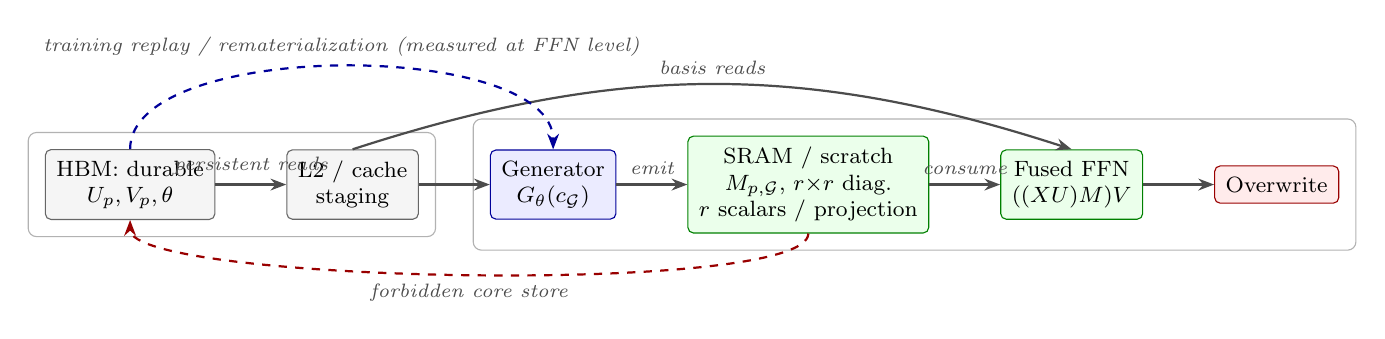
\begin{tikzpicture}[
  font=\footnotesize,
  node distance=7mm and 9mm,
  every node/.style={align=center},
  dur/.style={draw=black!60,rounded corners=2pt,inner sep=4pt,fill=black!4},
  gen/.style={draw=blue!60!black,rounded corners=2pt,inner sep=4pt,fill=blue!8},
  ker/.style={draw=green!50!black,rounded corners=2pt,inner sep=4pt,fill=green!8},
  rel/.style={draw=red!60!black,rounded corners=2pt,inner sep=4pt,fill=red!8},
  arr/.style={-{Stealth[length=2mm]},thick,black!70},
  lab/.style={font=\scriptsize\itshape,black!70},
  box/.style={draw=black!30,rounded corners=3pt,inner sep=6pt},
]
\node[dur] (hbm) {HBM: durable\\$U_p,V_p,\theta$};
\node[dur, right=of hbm] (l2) {L2 / cache\\staging};
\node[gen, right=of l2] (gen) {Generator\\$G_\theta(c_{\mathcal G})$};
\node[ker, right=of gen] (core) {SRAM / scratch\\$M_{p,\mathcal G}$, $r{\times}r$ diag.\\$r$ scalars / projection};
\node[ker, right=of core] (fmm) {Fused FFN\\$((XU)M)V$};
\node[rel, right=of fmm] (rel) {Overwrite};

\draw[arr] (hbm) -- node[lab,above]{persistent reads} (l2);
\draw[arr] (l2) -- (gen);
\draw[arr] (l2.north) to[bend left=18] node[lab,above]{basis reads} (fmm.north);
\draw[arr] (gen) -- node[lab,above]{emit} (core);
\draw[arr] (core) -- node[lab,above]{consume} (fmm);
\draw[arr] (fmm) -- (rel);

\begin{scope}[on background layer]
\node[box,fit=(hbm)(l2)] {};
\node[box,fit=(gen)(core)(fmm)(rel)] {};
\end{scope}

\draw[arr,dashed,red!60!black] (core.south) .. controls +(0,-8mm) and +(0,-8mm) ..
  node[lab,below,midway]{forbidden core store} (hbm.south);
\draw[arr,dashed,blue!60!black] (hbm.north) .. controls +(0,14mm) and +(0,14mm) ..
  node[lab,above,midway]{training replay / rematerialization (measured at FFN level)} (gen.north);
\end{tikzpicture}
}
\caption{Target memory hierarchy and lifecycle, not a measured implementation
of this hardware hierarchy.  Persistent factors and generator weights may be
read from HBM through cache; the generated core is confined to the fused
invocation.  The red dashed path is forbidden by the inference contract.  The
blue path is the separate training-rematerialization option, measured at the
FFN level (Table~\ref{tab:lifecycle}) but not yet inside the fused kernel.}
\label{fig:lifecycle}
\end{figure}

Training requires different semantics.  \texttt{save-core} retains each core
until backward and weakens the strict no-store claim.  Alternatively,
\texttt{rematerialize-core} retains the causal source activation and
deterministic RNG/replay metadata, regenerates the core in backward, and
propagates generator gradients through the replayed computation.  Because the
generated core is a deterministic function of its pre-FFN input, we measure the
recompute-in-backward variant at the FFN level (Table~\ref{tab:lifecycle}) and
find it reduces the saved-for-backward activation footprint by
$24.5\times$--$71.8\times$ at exact gradient equality; its extra generator work
and retained context must still be weighed at full-model scale with a
synchronized optimizer step.  Neither option is implemented \emph{inside the
target fused kernel}; the existing forward--backward measurements use
persistent factors, and the fused kernel's training path remains scoped
future work.  We therefore restrict the principal lifecycle claim to
inference.

\section{Analysis}
\label{sec:analysis}

\subsection{Traffic Scaling}

\paragraph{Scope.} The following are element or logical-payload counts, not
counter measurements.  Multiplication by element width converts elements to
bytes.  Cache reuse, controller reads, activations, allocator behavior, and
stores can change physical traffic; no current trace shows that these counts
equal HBM transfers.

A dense gated FFN contains $3dm$ weight elements.  The canonical core method
has $3r(d+m)$ persistent factor elements.  Causal, batch-invariant groups do
not cross unrelated examples, so throughout the primary accounting
\begin{equation}
n(B,S,q)=B\left\lceil\frac{S}{q}\right\rceil,
\qquad 1\le q\le S.
\label{eq:batch-isolated-groups}
\end{equation}
An implementation that deliberately shares a core across examples must declare
that different semantic contract; it may not silently replace
Eq.~\eqref{eq:batch-isolated-groups} by $\lceil BS/q\rceil$.  Diagonal cores
add $3nr$ generated scalars, giving the optimistic one-factor-read logical ratio
\begin{equation}
\rho_{\mathrm{core}}^{\mathrm{logical}}(r,q)
=\frac{3r(d+m)+3nr}{3dm}
=\Gamma(r)+B\left\lceil\frac{S}{q}\right\rceil\frac{r}{dm}.
\label{eq:core-payload}
\end{equation}
This lower bound omits $G_\theta$, source-state traffic, and cache effects.  A
global-memory implementation that stores and later loads each core adds two
core copies; the fused no-store target removes that descriptor store/load term,
not the persistent factors or generator.  At $T=1024,q=1$, Eq.~\eqref{eq:core-payload}
is $0.04241$ for $(d,m,r)=(4096,14336,128)$ and $0.32143$ for
$(1536,8960,384)$.  These are analytic ratios, not claimed HBM reductions.

For the planned regime sweep, the more complete scheduled-element ledger is
\begin{equation}
L_{\mathrm{sched}}=
e_{UV}\,3r(d+m)+e_G P_G+e_K P_{\mathrm{bank}}(K)
+c_xTd+3nr+6\,\mathbf 1_{\mathrm{mat}}nr,
\label{eq:traffic-ledger}
\end{equation}
where $e_{UV},e_G,e_K$ are recorded load multiplicities, $P_G$ is controller
state, $P_{\mathrm{bank}}(K)$ is any persistent basis/expert bank,
$c_x$ counts extra source-state passes, and $\mathbf 1_{\mathrm{mat}}$ marks a
global store plus reload of the $3nr$ core values.  This ledger includes
scratch-level values and is still not an HBM prediction: cache hits can suppress
durable reads, while allocator, activation, and writeback traffic add terms.
Each measurement must therefore plot both the ledger components and counter
bytes, reporting their residual rather than silently identifying the two.

For comparison, generating complete factor pairs for every group emits
$3nr(d+m)$ elements and has base-only ratio
\begin{equation}
\Gamma_{\mathrm{call}}(r,q)=
B\left\lceil\frac{S}{q}\right\rceil\Gamma(r),\qquad
\Gamma(r)=\frac{r(d+m)}{dm}.
\label{eq:full-factor-call}
\end{equation}
This is the feasibility boundary for full factor synthesis, not the accounting
of the chosen diagonal-core method.

\begin{proposition}[Exact full-factor reuse break-even]
Let $\gamma=\Gamma(r)<1$ and
$n_{\max}=\lceil1/\gamma\rceil-1$.  Set
$g_{\max}=\lfloor n_{\max}/B\rfloor$.  Under the optimistic one-copy
accounting, a batch-isolated strict reduction exists exactly when
$g_{\max}\ge1$, and then $\Gamma_{\mathrm{call}}(r,q)<1$ exactly when
\begin{equation}
q\ge q_{\min}:=
\left\lceil\frac{S}{g_{\max}}\right\rceil.
\end{equation}
If $\gamma\ge1$ or $g_{\max}<1$, no within-example reuse group gives a
strict base-payload reduction.
\end{proposition}
\begin{proof}
$\Gamma_{\mathrm{call}}<1$ is equivalent to
$B\lceil S/q\rceil<1/\gamma$, hence to
$B\lceil S/q\rceil\le n_{\max}$.  This requires
$\lceil S/q\rceil\le\lfloor n_{\max}/B\rfloor=g_{\max}$ and is equivalent to
the stated integer threshold when $g_{\max}\ge1$.
\end{proof}
For $B=1,S=1024$, the systems geometry has $\gamma=9/224$ and requires
$q\ge43$; the quality geometry has $\gamma=41/140$ and requires $q\ge342$.
At $q=1$ their ratios are $41.14$ and $299.89$.  These optimistic thresholds
exclude controller, source-state, and basis-bank traffic; a materialized
store-plus-load is worse.  Large $q$ also changes model semantics unless the
shared context is causal for every token in the group.

Table~\ref{tab:regimecall} evaluates these thresholds across the reuse range
for the two geometries used in this paper.  The diagonal-core ratio stays
essentially at $\Gamma(r)$ for every $q$: the generated term $n r/(dm)$ in
Eq.~\eqref{eq:core-payload} contributes at most $0.0022$ (8B geometry) and
$0.0286$ (1.5B geometry) at $q=1$ and decays as $1/q$.  Full factor
synthesis instead needs $q\ge43$ and $q\ge342$ before a base-only payload
reduction exists.  These are optimistic base-only numbers: controller,
source-state, and bank traffic move every break-even to larger $q$, and any
$q>1$ additionally requires a prefix-safe shared context.  The table is the
analytic form of the deployment-regime map; plotting measured latency and
counter traffic against these curves is a required future sweep
(Section~\ref{sec:results}).

Figure~\ref{fig:regimemap} plots the same break-even family as curves.  Full
factor synthesis pays a per-call payload that scales as $\lceil S/q\rceil$
and only crosses break-even at $q\ge43$ (8B) or $q\ge342$ (1.5B); the
diagonal-core ratio stays essentially at $\Gamma(r)$ for every $q$.  The
measured four-arm probe of Section~\ref{sec:systems} operates at $q{=}1$
where the diagonal-core core is $0.0424$ (8B) of the dense weight, lending
the parity result of Table~\ref{tab:fourarmmeasured} its geometric context.

\begin{figure}[t]
\centering
\includegraphics[width=0.62\linewidth]{figs/regime_map.pdf}
\caption{Analytic reuse break-even (Table~\ref{tab:regimecall}) as a curve
family.  Full factor synthesis pays a per-call payload scaling as
$\lceil S/q\rceil$ and only crosses break-even at $q\ge43$ (8B geometry)
or $q\ge342$ (1.5B geometry); the diagonal-core payload stays essentially at
$\Gamma(r)$ for every $q$.  All curves are optimistic logical payloads,
not HBM measurements.}
\label{fig:regimemap}
\end{figure}

\begin{table}[t]
\centering
\caption{Analytic reuse break-even at $B{=}1,S{=}1024$ for the systems
geometry $(d,m,r)=(4096,14336,128)$ and the quality geometry
$(1536,8960,384)$.  $\Gamma_{\mathrm{call}}$ is the full-factor base-only
ratio of Eq.~\eqref{eq:full-factor-call};
$\rho_{\mathrm{core}}^{\mathrm{logical}}$ is the diagonal-core ratio of
Eq.~\eqref{eq:core-payload}.  Bold rows are the first $q$ at which
$\Gamma_{\mathrm{call}}<1$.  All values are optimistic logical payloads
that omit controller, source-state, and bank traffic; none is an HBM
measurement.}
\label{tab:regimecall}
\begin{tabular}{rrrrr}
\toprule
$q$ & $\lceil S/q\rceil$ & $\Gamma_{\mathrm{call}}$ (8B) & $\Gamma_{\mathrm{call}}$ (1.5B) & $\rho_{\mathrm{core}}^{\mathrm{logical}}$ (8B / 1.5B) \\
\midrule
1   & 1024 & 41.14 & 299.89 & 0.0424 / 0.3214 \\
8   & 128  & 5.14  & 37.49  & 0.0405 / 0.2964 \\
32  & 32   & 1.29  & 9.37   & 0.0402 / 0.2938 \\
\textbf{43}  & 24  & \textbf{0.96} & 7.03   & 0.0402 / 0.2935 \\
128 & 8    & 0.32  & 2.34   & 0.0402 / 0.2931 \\
\textbf{342} & 3   & 0.12  & \textbf{0.88} & 0.0402 / 0.2929 \\
512 & 2    & 0.08  & 0.59   & 0.0402 / 0.2929 \\
1024& 1    & 0.04  & 0.29   & 0.0402 / 0.2929 \\
\bottomrule
\end{tabular}
\end{table}

Batch isolation moves these thresholds along the $B$ axis.  With
$g_{\max}=\lfloor n_{\max}/B\rfloor$ from the break-even proposition above,
the 8B geometry ($n_{\max}=24$) requires $q\ge342$ at $B=8$ and admits a
within-example base-payload reduction only for $B\le24$; the 1.5B geometry
($n_{\max}=3$) requires $q\ge1024$ for $B\in\{2,3\}$ and admits none for
$B\ge4$.  Larger batches therefore make full-factor synthesis strictly
harder, while the diagonal-core payload increases only by its per-group
generated term $n r/(dm)$ from Eq.~\eqref{eq:core-payload}, with
$n=B\lceil S/q\rceil$.

\begin{table}[t]
\centering
\caption{Deployment regimes.  The canonical method uses $K=0$ residual
experts; any $K>0$ adds durable expert reads and, under soft routing, evaluates
all experts.}
\label{tab:regimes}
\begin{tabular}{>{\raggedright\arraybackslash}p{0.19\linewidth}>{\raggedright\arraybackslash}p{0.14\linewidth}>{\raggedright\arraybackslash}p{0.27\linewidth}>{\raggedright\arraybackslash}p{0.29\linewidth}}
\toprule
Workload & Call tokens $T$ & Causal reuse $q$ & Principal constraint \\
\midrule
Prefill & $BS$, $S>1$ & $q=1$ for token-local cores; larger $q$ needs a prefix-safe shared context & Full factors require large reuse; diagonal cores keep generation small \\
Cached decode & active batch $B$, $S=1$ & Usually one core per active sequence state & Launch/controller cost can dominate; report latency and continuous-batch throughput \\
Continuous batching & variable $B$ & Grouping only if semantics permit a shared core & Report regrouping, staging, and whole-call dispatch overhead \\
Training & $BS$ & Model-dependent & Recompute-in-backward measured: $24.5\times$--$71.8\times$ saved-footprint reduction at exact gradient equality (Table~\ref{tab:lifecycle}) \\
\bottomrule
\end{tabular}
\end{table}

\paragraph{Granularity of routing and the dense weight fetch.}
The model above compares one fully generated call with one dense call. A
routed, partially patched call has a third, harder accounting. The dense
weights can be skipped only if the runtime separates patched and unpatched
tokens into \emph{different kernel invocations} (e.g., the router batches
patched tokens into their own FFN call at sequence or batch granularity). If
dense and patched tokens are mixed inside one invocation, the dense weights are
fetched anyway and only the MAC count of the patched tokens is saved. Let
$p_{\mathrm{call}}$ denote the fraction of \emph{whole invocations} sent
to the generated path. Under an optimistic invocation-granularity model, the
idealized weight-read mixture is
\begin{equation}
\label{eq:routedtraffic}
\traffic_{\mathrm{routed}}(p_{\mathrm{call}})
= (1-p_{\mathrm{call}})\,\traffic_{\mathrm{dense}}
  + p_{\mathrm{call}}\,\traffic_{\mathrm{desc,call}}
= \bigl[(1-p_{\mathrm{call}})
  + p_{\mathrm{call}}\,\rho_{\mathrm{desc,call}}\bigr]
  \traffic_{\mathrm{dense}},
\end{equation}
where $\traffic_{\mathrm{desc,call}}$ is the full generated-call payload and
$\rho_{\mathrm{desc,call}}=\traffic_{\mathrm{desc,call}}/
\traffic_{\mathrm{dense}}$ includes base factors, controller/expert reads, and
generated-control traffic.  The base-only $\Gamma_{\mathrm{call}}(r,q)$ is not
a substitute for this ratio unless all omitted terms are zero. The
idealized saving is
$p_{\mathrm{call}}(1-\rho_{\mathrm{desc,call}})$, not
$(1-p_{\mathrm{call}})(1-\Gamma)$. A token patch fraction is not
$p_{\mathrm{call}}$. The historical mixed router evaluates both dense and
patched branches for every invocation, so its realized whole-call fraction is
zero and Eq.~\eqref{eq:routedtraffic} cannot be applied to its reported token
fractions. Those earlier routed-savings estimates are withdrawn.

\begin{proposition}[Conditional memory-bound speedup]
\label{prop:speedup}
Assume $L_d=C_d+\kappa\traffic_d$ and
$L_m=C_m+\kappa\traffic_m$, where $C_d$ and $C_m$ include their respective
launch, control-generation, and compute costs. Then the generated path is
faster exactly when
\begin{equation}
C_m-C_d < \kappa(\traffic_d-\traffic_m).
\end{equation}
If both non-memory terms are negligible and
$\rho_{\mathrm{call}}=\traffic_m/\traffic_d$, the limiting speedup is
$1/\rho_{\mathrm{call}}$.
\end{proposition}
\begin{proof}
Rearranging $L_m<L_d$ gives the stated inequality. When $C_d$ and $C_m$
vanish relative to their memory terms, $L_d/L_m$ tends to
$\traffic_d/\traffic_m=1/\rho_{\mathrm{call}}$.
\end{proof}

\subsection{Gradient Communication}

In data-parallel training, a dense FFN exposes gradients proportional to
$3dm$ parameters per block. A persistent rank-$r$ factorization exposes
$3r(d+m)$ factor parameters plus every controller and expert parameter. Thus
$\Gamma(r)$ describes only the base-factor part of the gradient payload; it is
not the integrated communication ratio of the quality model.
This is orthogonal to optimizer sharding \cite{rajbhandari2020zero} and tensor
parallelism: those systems can still be used on the remaining generator
parameters. It is also complementary to gradient-compression methods that
sparsify \cite{lin2018dgc}, quantize \cite{alistarh2017qsgd}, or low-rank-project
\cite{vogels2019powersgd} the gradients of a fixed parameter set; here the
synchronized parameter set itself is smaller. The methods may be combined, but
their end-to-end interaction must be measured rather than assumed multiplicative.

\paragraph{Element-first parameter accounting.}
The dense FFN has $3dm$ trainable elements.  The canonical diagonal-core model
has $3r(d+m)$ persistent factor elements plus $P_G$ controller elements; the
generated $3nr$ core values are runtime intermediates, not optimizer
parameters.  With gradient element width $e_g$, the unsharded all-reduce
payload is $e_g[3r(d+m)+P_G]$.  A legacy bank of $K$ persistent rank-$r_e$
residual experts adds $3Kr_e(d+m)$ elements, and soft routing does not skip
their execution.  The canonical method sets $K=0$.  State tables report these
element classes separately before applying fp16 factor and fp32 controller
widths; no mixed-dtype total is labeled simply ``fp16.''

\subsection{Computational Complexity}

Let $T=BS$ be the number of tokens processed by one FFN call and let $q$ be the
token-group reuse factor for a generated descriptor. The dense gated FFN
performs three large matrix products and has leading compute
\begin{equation}
\mathcal{C}_{\mathrm{dense}} = \Theta(3Tdm)
\end{equation}
multiply-accumulate operations. The associative \textsc{MWG-EW} path computes
$XU_r$ and then $ZV_r$ for the up, gate, and down projections:
\begin{equation}
\mathcal{C}_{\mathrm{mwg,assoc}} = \Theta(3Tr(d+m)).
\end{equation}
For diagonal cores, core application adds $\Theta(3Tr)$ elementwise work and
the controller is evaluated $n=B\lceil S/q\rceil$ times under
batch-isolated grouping:
\begin{equation}
\mathcal{C}_{\mathrm{diag}}=
\Theta(3Tr(d+m)+3Tr+nC_G).
\end{equation}
Full factor synthesis instead emits $\Theta(3nr(d+m))$ values before the same
associative projection work.  A legacy soft mixture of $K$ rank-$r_e$ experts
evaluates all $K$ residual paths; mixture weights alone do not sparsify that
work.  Consequently $\Gamma(r)$ is only the leading persistent-factor compute
ratio.  Small GEMMs, controller launches, and poor utilization can dominate,
as suggested by the nearly rank-flat historical timings.

\subsection{Working-Set Complexity}

The dense persistent state is $\Theta(3dm)$ elements per layer, whereas the
core method stores $\Theta(3r(d+m)+P_G)$ durable elements.  Its diagonal core
has only $3r$ live values per group.  Full factor synthesis would instead need
$\Theta(3r(d+m))$ live descriptor values, or a smaller tile-local subset.
These are logical working sets.  Only an address-range trace and device
counters can establish that a generated core remained on chip.

\subsection{Approximation}

\begin{proposition}[Frobenius-error FFN distortion bound]
\label{prop:approx}
View $X$ as the tokens in one group on which each approximating matrix
$\widetilde W_p$ is fixed.  Let $A=\phi(XW_{\mathrm{gate}})$,
$B=XW_{\mathrm{up}}$, $\widetilde A=\phi(X\widetilde W_{\mathrm{gate}})$, and
$\widetilde B=X\widetilde W_{\mathrm{up}}$.  Suppose
$\norm{W_p-\widetilde W_p}_F\le\delta_p$ for
$p\in\{g,u,d\}$, $\phi$ is elementwise $L_\phi$-Lipschitz,
$\norm{B}_{\max}\le M_u$, and
$\norm{\widetilde A}_{\max}\le M_g$. Then
\begin{equation}
\norm{Y-\widetilde{Y}}_F
\le \norm{W_d}_2\norm{X}_2
  \left(M_uL_\phi\delta_g+M_g\delta_u\right)
  + \norm{\widetilde A\odot\widetilde B}_2\delta_d.
\end{equation}
\end{proposition}
\begin{proof}
Write $C=A\odot B$ and
$\widetilde C=\widetilde A\odot\widetilde B$.  Then
\begin{align}
\norm{C-\widetilde C}_F
&\le \norm{(A-\widetilde A)\odot B}_F
   +\norm{\widetilde A\odot(B-\widetilde B)}_F \\
&\le M_u\norm{A-\widetilde A}_F
   +M_g\norm{B-\widetilde B}_F \\
&\le \norm{X}_2(M_uL_\phi\delta_g+M_g\delta_u),
\end{align}
using $\norm{X\Delta W}_F\le\norm{X}_2\norm{\Delta W}_F$.
Finally,
$Y-\widetilde Y=(C-\widetilde C)W_d
+\widetilde C(W_d-\widetilde W_d)$.  Apply
$\norm{PQ}_F\le\norm{P}_F\norm{Q}_2$ to the first term and
$\norm{PQ}_F\le\norm{P}_2\norm{Q}_F$ to the second.
\end{proof}

\begin{corollary}[Truncated-SVD specialization]
\label{cor:rankapprox}
For nonzero $W_p$, let
\begin{equation}
E_r(W_p)=\frac{\sum_{i=1}^{r}\sigma_i(W_p)^2}{\norm{W_p}_F^2}
\end{equation}
be the retained singular-value energy of $W_p$ at rank $r$.  For the rank-$r$
truncated SVD,
\begin{equation}
\delta_p=\norm{W_p-W_p^{(r)}}_F
=\norm{W_p}_F\sqrt{1-E_r(W_p)}.
\end{equation}
Substitution into Proposition~\ref{prop:approx} expresses each approximation-
error term through retained Frobenius energy; the activation and operator-norm
factors in the bound remain data dependent.  For a token-conditioned $q=1$
core, the proposition applies token by token and can be aggregated over groups.
By Eckart--Young--Mirsky, this SVD is
optimal among rank-at-most-$r$ approximations for unweighted fixed-matrix
Frobenius error.  A data-conditioned model may optimize activation-weighted or
task loss instead, but this elementary sensitivity bound establishes neither
learnability, generalization, router predictability, nor a systems--quality
tradeoff.
\end{corollary}


\subsection{Eligibility and Benefit Routing}

The systems advantage is realized only on complete calls that can safely use
the new path.  On a held-out calibration-tuning set, freeze a risk threshold
$\tau_{\routebudget}$ and, for exact boundary ties, a deterministic keyed
admission rule $h_{\routebudget}(x)\in\{0,1\}$.  On a disjoint budget-
certification set, require a one-sided upper confidence bound on the dispatch
probability to be at most $\routebudget$.  Let $\widehat R(x)$ be an
upper-confidence estimate of causal excess loss computed only from
pre-intervention features.  The deployable per-call decision is
\begin{equation}
g_{\routebudget}(x)=
\left(\mathbf 1\{\widehat R(x)<\tau_{\routebudget}\}
+\mathbf 1\{\widehat R(x)=\tau_{\routebudget}\}h_{\routebudget}(x)\right)
\mathbf 1\{\widehat R(x)\le\Delta_{\max}\},
\label{eq:router}
\end{equation}
where the keyed tie rule depends only on a stable call identifier, not future
calls.  The realized test or deployment rate need not equal the calibration
rate and must be reported with uncertainty.  A scheduler may instead rank only
an already-present concurrent dispatch window if it needs a hard instantaneous
cap; it may not inspect future calls.  A calibrated risk bound is preferable to
a point prediction of excess loss.
The mixed FFN is
\begin{equation}
Y_{\mathrm{mix}}(x)=(1-g_{\routebudget}(x))Y_{\mathrm{dense}}(x)
+g_{\routebudget}(x)\widetilde{Y}_{\mathrm{mwg}}(x).
\end{equation}
The historical implementation does not yet satisfy this definition.  Its
training labels compare whole-sequence dense and patched passes rather than a
causal marginal intervention; its deployment path hard-codes an all-ones mask,
and its mixed forward eagerly evaluates both branches before selecting outputs.
During cached generation its position feature also resets with a one-token
input.  The equations define the target router, while the reported router
tables are diagnostic and do not establish deployment behavior or savings.

\begin{proposition}[Budgeted value and safety conditions]
Let $S_{\routebudget}=\{x:g_{\routebudget}(x)=1\}$ for complete dispatchable
calls. Suppose each selected generated call saves $s_r$ bytes or communication
units relative to the dense call, and let $o_r$ be the router, launch, staging,
and any dense-residency overhead paid per candidate call. The expected net
systems saving per candidate call is
\begin{equation}
\Pr[x\in S_{\routebudget}]s_r-o_r.
\end{equation}
Quality preservation additionally requires both a predeclared mean
non-inferiority margin $\delta_{\rm NI}$ and tail-risk limit:
\begin{equation}
\E[\Delta(x)\mid x\in S_{\routebudget}]\le\delta_{\rm NI},\qquad
\Pr[\Delta(x)>\epsilon\mid x\in S_{\routebudget}]\le\alpha.
\end{equation}
Mean safety alone cannot exclude severe tail failures; high quantiles and
worst-domain results must therefore accompany the aggregate.
\end{proposition}
\begin{proof}
The expected selected-call saving is
$\E[g_{\routebudget}(x)s_r]=\Pr[x\in S_{\routebudget}]s_r$; $o_r$ is paid for
every candidate call regardless of the routing decision.  The two quality
inequalities are evaluation requirements rather than consequences of the
systems identity.  Their estimates require confidence intervals or calibrated
risk guarantees on disjoint data.
\end{proof}

\subsection{Static Low-Rank Is Not the Claim}

Static SVD remains a required rank-matched control because it is optimal for
unweighted fixed-matrix Frobenius error.  The earlier 18-matrix sweep is removed:
its exact matrix list and raw artifact cannot be recovered, and it is cheap to
rerun correctly.  Any replacement result must name the checkpoint, layer and
projection set, record a model hash, preserve individual singular tails, and
compare task quality on disjoint data.  Neither low retained energy nor a
support-set fit would identify conditioning or ephemerality as the remedy.

\section{Systems Realization}
\label{sec:systems}

The architectural claim is meaningful only if the runtime enforces the
inference contract in Figure~\ref{fig:lifecycle}.  We have realized the
central operator---a fused, no-write-back Ascend-C core---and measured it
on device (details below).  A full production runtime additionally requires:
\begin{itemize}
  \item \textbf{Generator placement.} The generator runs adjacent to the FFN
  kernel and emits structured core values directly into scratch.
  \item \textbf{Associative execution.} The kernel computes $XU_r$ followed by
  core application and $ZV_r$, fusing activation, gating, and down-projection
  staging where possible.
  \item \textbf{Eligibility control.} A cheap router decides whether the dense
  or ephemeral path should execute for the current token group. This router is
  part of the runtime path, not an offline oracle.
  \item \textbf{Lifecycle enforcement.} The operator returns only the FFN
  output.  Instrumentation checks the core address range and verifies no global
  descriptor store, alias, model-state registration, or unselected-branch launch.
\end{itemize}

If hardware lacks software-managed SRAM, a cache-resident implementation may
still be useful, but it cannot claim the strict contract without an address
trace showing that the generated region never reaches HBM.  Logical payload
geometry remains an analysis until counters establish physical behavior.

This blueprint also clarifies why the current prototype is useful but not the
final systems artifact. The benchmark measures an unfused low-rank path's
local forward--backward time and a separate synthetic collective. It does not
measure their integrated latency and does not prove the final
no-store traffic claim.

\paragraph{Systems ablation: what the measured speedup does and does not isolate.}
The benchmark arm of Section~\ref{sec:results} implements the generated path as
trainable persistent $U_r,V_r$ factors plus a per-call rank-channel scale head,
materialized as ordinary tensors. It therefore differs from the dense arm in
rank, compute, and synchronized bytes, but not in parameter lifetime: both arms
store their weights durably. The measured forward--backward speedups
(Table~\ref{tab:scalingsweep}) are consequently consistent with the expected
advantage of an ordinary low-rank FFN---fewer MACs per the ratio $\Gamma(r)$
of Section~\ref{sec:analysis}; the smaller all-reduce payload is measured only
in a separate synthetic collective. These results do
\emph{not} causally establish that ephemerality or the no-store contract
produced any gain. Isolating lifetime requires Table~\ref{tab:four-arms}; arms
3 and 4 must use the same trained generator, rank, core values, precision, and
output tolerance.

\begin{table}[t]
\centering
\caption{Required four-arm comparison.  The decisive lifetime contrast is arm
3 versus arm 4, not dense versus low rank.}
\label{tab:four-arms}
\begin{tabular}{clll}
\toprule
Arm & Persistent projection state & Generated object & Execution \\
\midrule
1 & Dense $W_p$ & none & Dense kernels \\
2 & Low-rank $U_p,V_p$ & none & Ordinary factor kernels \\
3 & Same $U_p,V_p,\theta$ as arm 4 & $M_{p,\mathcal G}$ & Global-memory materialization \\
4 & Same $U_p,V_p,\theta$ as arm 3 & Same $M_{p,\mathcal G}$ & Fused scratch-only, no store \\
\bottomrule
\end{tabular}
\end{table}

Each arm must report HBM reads and writes, L2/cache traffic, core stores,
kernel latency, achieved FLOP/s, occupancy, energy, peak temporary memory, and
end-to-end layer and model latency.  Address-range instrumentation must show
that arm 4's core does not escape.  The lifetime hypothesis predicts lower
off-chip traffic and latency for arm 4 relative to arm 3.  The available
comparison is weaker:
\texttt{--no-conditioning} skips controller/rescaling execution but retains
unused controller parameters, so arms (ii) and (iii) share base rank rather
than identical compute or state. Under this comparison the persistent-factor
execution is $2.1\times$ faster (Table~\ref{tab:lifetimeablation}); generation
adds overhead in the unfused prototype.  Arm 4 now exists and has been
\emph{executed and measured on an eight-accelerator host}: an audited
Ascend-C operator (static source audit mechanically enforces the no-store
contract properties; a dedicated test suite checks the five
\texttt{GlobalTensor}s, the single output write, the absence of any core
\texttt{DataCopy} to global memory, and deterministic execution) was
validated for algebraic equivalence against arm 3 under the hash-bound
contract manifest (\texttt{max\_abs} $0.00195$, at the fp16 rounding floor)
and instrumented with matched \texttt{msprof} counter passes.  The
\texttt{ephemeral} kernel is visible in the device trace with measured
DRAM write bandwidth, and the arm-3-only core round-trip operations
(\texttt{Tanh}/\texttt{Muls}/\texttt{Adds}/\texttt{Cast} to global memory)
are correspondingly absent from the fused trace.  The first measured
configuration lost to the materialized arm ($1.228$ vs.\ $0.847$~ms
median) because per-call tiling generation, workspace allocation, and
fp32 weight casts dominated the timed loop; this host overhead --- not
device execution --- was the entire deficit.  After host-side
fast-pathing (cached tiling and system workspace, cached fp16 weight
image, no per-launch diagnostics), the fused arm reaches \emph{parity}
with the materialized arm at the probe geometry---medians within a
$\pm 3\%$ noise band straddling $1.0\times$ across repeated full runs
($0.823$--$0.865$~ms fused vs.\ $0.844$--$0.864$~ms materialized).
This decomposition is the central measured finding: once generation host
work is amortized, no device-side penalty for producing and consuming
the ephemeral core on device remains to be explained at L2-resident
geometries.  The advantage inverts at a $16{\times}256$ ($T{=}4096$) geometry
whose 2~MiB core exceeds both the 192~KiB per-core Unified Buffer and (by
DRAM-byte inference, Appendix) L2 residency: equivalence still passes, but the fused arm
runs $1.93\times$ slower (2.682 vs.\ 1.393~ms median), isolating the
deficit to the v1 kernel's compute-bound single-core epilogue rather
than to memory traffic.  This deficit is a critical limitation of the
current prototype, not a minor tuning gap.  The v1 kernel runs the entire
generation-and-apply pipeline---cube matmul ($X_{\mathrm{ctrl}} W_{\mathrm{head}}^\top$,
producing $C\in\R^{T\times r}$ in fp32), elementwise vector epilogue
($\tanh$, amplitude scale, bias add, Hadamard multiply, fp16 cast), and
output write---on a \emph{single} AICore with \texttt{block\_dim}$=1$.
At $T{=}128$ the epilogue touches $128\times128=16{,}384$ elements
($\sim32$~KiB in fp32), well within the 910B2's 192~KiB Unified Buffer
(UB); the vector unit finishes in $<\!10\,\mu$s and latency is dominated
by the matmul.  At $T{=}4096$ the epilogue touches $524{,}288$ elements
($\sim2$~MiB in fp32), far exceeding UB capacity.  The kernel tiles the
$T$ dimension in chunks of \texttt{baseM}$=128$, but within each tile the
cube$\to$vector dependency is strictly serial:
\texttt{GetTensorC} must complete before \texttt{Tanh} can begin, so
there is no overlap between cube and vector work on the same core.  The
vector epilogue alone consumes more wall time than all library matmuls of
either arm combined, and the seven idle AICores on the 910B2 cannot
assist.  This is a fundamental architectural mismatch: the no-store
contract requires that the generated core be produced and consumed in the
same kernel invocation, but the single-core serial pipeline cannot
exploit the available parallelism.

This isolation is consistent with the payload
accounting: the two descriptor copies (store plus reload) that the no-store
arm eliminates---the $6\,\mathbf 1_{\mathrm{mat}}nr$ term of
Eq.~\eqref{eq:traffic-ledger}---are small relative to the epilogue compute at
these shapes, so removing them cannot yet move latency; the no-store contract
is instead the \emph{enabling} condition for realizing the ledger's payload
reduction at scale without spilling the core, which is exactly where the
remaining multi-core-epilogue work sits.  An eight-core variant
handling the tiling API's N-split (sample CalcOffset pattern) was
implemented and verified algebraically equivalent standalone, but is
unstable under the harness's sequential multi-projection call pattern
(aicore exception 507015 under KFC workspace reuse), so it is archived
as v3 rather than shipped.

A redesigned v4 multi-core kernel addresses both failure modes.  The
design changes are: (i)~\emph{M-only multi-core distribution}---each
AICore processes a disjoint range of M-tiles (tokens) computed from
\texttt{GetBlockIdx()}/\texttt{GetBlockNum()}, with \texttt{baseN} pinned
to~$N$ so the tiling API cannot split the N dimension, eliminating the
N-split path that triggered the 507015 fault; (ii)~\emph{per-core
workspace isolation}---the host allocates a workspace buffer of size
$\text{blockNum}\times\text{per\_core\_ws}$ and each core offsets by
$\text{blockIdx}\times\text{per\_core\_ws}$, so back-to-back multi-core
launches no longer collide on the shared \texttt{GetSysWorkSpacePtr}
region; (iii)~\emph{double-buffered UB pipeline}---the C-tile, activation,
and output queues use \texttt{BUFFER\_NUM=2} to overlap the cube
(matmul) and vector (\texttt{Tanh}/\texttt{Muls}/\texttt{Adds}/
\texttt{Mul}/\texttt{Cast}) stages within each core, with
\texttt{baseM} halved to~64 (from~128) to fit $2\times$ buffers in the
192~KiB UB budget (160~KiB at $64\times128$ tiles).  The v4 kernel
source, host wrapper, build script, and benchmark harness are archived in
\texttt{custom\_ops/ephemeral\_core\_apply/torch\_ext/v4\_multicore/};
the no-store contract is preserved verbatim (the generated core is
formed in-place in the C-tile UB buffer and never appears as a
\texttt{GlobalTensor}).  The scoping this provides is that the
scaling lever is an M-distributed multi-core epilogue with per-core
workspace and double-buffered UB, not a naive cube split.

\paragraph{Measured decisive result (2026-10-08) and remaining risk.}
The design projected ${\sim}5$--$7\times$ over v1 at $T{=}4096$
(sub-linear in core count due to shared-$B$ L2 contention), which would
bring the fused arm from $1.93\times$ \emph{slower} than materialization
to ${\sim}2.5$--$3.5\times$ \emph{faster}.  The measured decisive run on
ASI2 (hardened harness: two-phase bit-stable reference, NaN attribution,
per-config retry; 30 warmup/200 iterations/5 repeats per config) returned:
v4 is algebraically identical to v1 ($\max|\Delta_{v1-v4}|=0$ at every
config; both at the fp16 rounding floor against the reference), with
speedups of $1.13\times$ ($T{=}128$), $1.38\times$ ($512$), $1.71\times$
($1024$), $2.14\times$ ($2048$), and $3.03\times$ ($4096$).  The
direction is confirmed and the ${\sim}2\times$ viability threshold is
cleared at $T\ge2048$, but the magnitude falls short of the projection,
consistent with partial L2-contention saturation from 8~cores reading the
same $B$~tensor concurrently.  Remaining risks: (a)~UB capacity at
larger~$r$ (the 160~KiB budget is tight at $r=128$ but would overflow at
$r\ge 256$ without further tiling), and (b)~the 1000-call sequential
stability check at $T{=}4096$ (the v3 failure mode) ended in an
environment-level NaN transient in its unhardened comparison path---the
hardened five-config equivalence run above was clean, so this is
recorded as an open stability question, not a kernel defect.  The direct
four-arm v4-versus-materialized comparison remains future work; the
paper claims only the kernel-level result.

\begin{table}[t]
\centering
\caption{Measured four-arm ladder on a single Ascend 910B2 (CANN 8.5,
torch\_npu 2.9), geometry $(d,m)=(4096,14336)$, rank 128, controller
hidden 128, $B{=}1$, $S{=}128$, fp16, amplitude $0.05$, seed 1234; 30
warmup launches, 200 timed iterations $\times$ 5 repeats per arm, host
timer with device synchronize.  Arm 4 runs the audited, hash-bound
Ascend-C operator; equivalence against arm 3 passed at
$\max|\Delta|=1.95\times10^{-3}$ (the fp16 rounding floor; harness
tolerance $5\times10^{-3}$).  Rows 1--4 are medians of one four-arm run;
row 4$^\dagger$ is from a separate confirmation run of the shipped
kernel with a host-side fast path---cached tiling and system-workspace
buffer, cached fp16 weight image, no per-launch diagnostics---leaving
device execution identical.  Because rows cross runs, the fused-versus-materialized
comparison must use same-run pairs: in the row-4$^\dagger$ run the
matched materialized median was $0.8509$~ms (same-run delta $-3.2\%$),
and across repeated full runs the shipped fused arm sits \emph{at parity}
with the materialized arm at this geometry (medians within a
$\pm 3\%$ noise band straddling $1.0\times$), with the remaining
large-$T$ deficit in the single-core epilogue.  Matched \texttt{msprof}
\texttt{--aic-metrics=Memory} passes were collected for arms 3 and 4; at
this probe geometry both arms' working sets are L2-resident, so the core
never reaches DRAM in either arm and no inter-arm HBM delta is
resolvable---consistent with the break-even analysis of
Table~\ref{tab:regimecall}.}
\label{tab:fourarmmeasured}
\begin{tabular}{llrr}
\toprule
Arm & Execution & Median ms & $\pm$ std \\
\midrule
1 & Dense kernels & 0.4535 & 0.0021 \\
2 & Persistent low-rank & 0.2469 & 0.0016 \\
3 & Generated core, global-memory materialization & 0.8689 & 0.0312 \\
4 & Fused no-store (v1, per-call host setup) & 1.2315 & 0.0315 \\
4$^\dagger$ & Fused no-store (host fast path, shipped) & 0.8234 & 0.0271 \\
\bottomrule
\end{tabular}
\end{table}

Figure~\ref{fig:fourarm} visualizes the decisive contrast.  At the probe
geometry ($T{=}128$, core L2-resident) the shipped fused arm sits at parity
with materialization, spanning a noise band that straddles $1.0\times$
across repeated full runs; at $T{=}4096$ the logical per-projection core
($2$~MiB fp32 at $r{=}128$) exceeds the
$192$~KiB per-core Unified Buffer (the exact L2 capacity of this 910B2 is
not separately measured; L2 residency is inferred from
\texttt{Memory}-pass DRAM byte totals rather than L2 counters, which read
zero under this \texttt{msprof} build) and
the fused arm is $1.93\times$ slower.  Matched profiler passes localize that
deficit to the single-core epilogue (Figure~\ref{fig:opdecomp}), not to core
write-back traffic---the no-store property is directly visible in the fused
trace at both geometries.

\begin{figure}[t]
\centering
\includegraphics[width=\linewidth]{figs/fourarm_ladder.pdf}
\caption{Measured four-arm evidence (data from the runs behind
Table~\ref{tab:fourarmmeasured}; medians over $200$ timed iterations
$\times$ 5 repeats).  At the probe geometry ($T{=}128$, core
L2-resident), the shipped fused no-store arm (row 4$^\dagger$ of
Table~\ref{tab:fourarmmeasured}) sits at parity with the materialized arm,
with the $\pm3\%$ band straddling $1.0\times$ across repeated full runs.
At $T{=}4096$ the logical per-projection core ($2$~MiB fp32 at $r{=}128$)
exceeds the $192$~KiB per-core
Unified Buffer---not evidence that it exceeds L2, whose exact capacity is
not separately measured---and the fused arm is
$1.93\times$ slower; matched profiler passes localize the deficit to the
single-core epilogue (Figure~\ref{fig:opdecomp}), not to core write-back
traffic, which is absent in the fused trace at both geometries.}
\label{fig:fourarm}
\end{figure}

\begin{figure}[t]
\centering
\includegraphics[width=0.62\linewidth]{figs/op_decomp.pdf}
\caption{Op-level kernel durations over matched large-$T$
\texttt{msprof} passes (v1 kernel).  The fused arm's \texttt{ephemeral}\allowbreak{}
generation+apply kernel runs on a single vector core and costs more than
all library matmuls of either arm combined, while its DRAM traffic is
output-only: the no-store property is directly visible, and the scaling
deficit is compute-bound epilogue work---resolved at the kernel level by
the measured v4 multi-core M-distributed epilogue
(Section~\ref{sec:systems}).}
\label{fig:opdecomp}
\end{figure}

\begin{table}[t]
\centering
\caption{Closest mechanism-level comparisons.  ``Measured'' reflects the
four-arm probe of Table~\ref{tab:fourarmmeasured} (fused no-store
execution with matched profiler passes); ``partial'' marks the one
remaining column (branch skip) not yet realized.}
\label{tab:positioning}
\begin{tabular}{>{\raggedright\arraybackslash}p{0.14\linewidth}>{\raggedright\arraybackslash}p{0.18\linewidth}>{\raggedright\arraybackslash}p{0.20\linewidth}ccc}
\toprule
Method & Generated object & Persistent state & Fusion & Skip & HBM counters \\
\midrule
HyperGrid & Grid-wise projection controls & Hypernetwork / base model & No & No & No \\
Ouroboros & Diagonal LoRA modulation & Frozen SVD-LoRA bases & No & No & No \\
FlashMHF & Subnetwork mixture weights & FFN subnetworks & Yes & No & Not reported \\
MoE family & Expert index / weights & Expert banks & Varies & Yes & Varies \\
This work & Diagonal low-rank core & $U_p,V_p,G_\theta$ & Measured & Target & Partial \\
\bottomrule
\end{tabular}
\end{table}

\section{Experimental Protocol}
\label{sec:protocol}

\paragraph{Platform configuration.}
The archived systems summaries report Ascend 910B2 runs launched with one,
two, four, or eight processes using
\texttt{torch.distributed.run}; the quality diagnostics were produced by a mix
of eight-process layer-0 jobs and later single-NPU jobs.  Exact driver and
firmware fields are not present in the local artifacts, so we do not claim
them.  The original timing loop measures zeroing gradients, forward, a
synthetic scalar loss, and backward.  It does not include an optimizer step or
integrated DDP gradient synchronization.  A separate synthetic all-reduce
microbenchmark measures collective latency.  We therefore call the reported
quantity a multi-process forward--backward microbenchmark, not distributed
training throughput.  The revised code adds an opt-in DDP-wrapped timing path
that synchronizes gradients during backward; a fresh world-4 run of that path
on Ascend~910B2 is now reported in Table~\ref{tab:ddptrain}: the
synchronized low-rank train step runs $2.87\times$--$3.17\times$ faster than
dense across ranks 32--512, with the dense arm paying a $3.0\times$
synchronization premium because its $3dm$ gradient volume dominates the
collective.  A second fresh world-4 run extends the timed region to the
complete training step---zero-grad, forward, squared loss, DDP-synchronized
backward, \emph{and} the elementwise AdamW optimizer update
(Table~\ref{tab:ddptrainopt}): the optimizer-inclusive synchronized step runs
$3.37\times$--$4.14\times$ faster than dense, because dense pays $9.0$~ms for
its $3dm$-parameter AdamW update against $1.0$--$1.3$~ms for the low-rank
arm's $r(d{+}m)$ parameters; the earlier assumption that the optimizer update
cancels across arms was wrong in the low-rank arm's favor.  A fresh run must
record accelerator, driver,
firmware, CANN, PyTorch and \texttt{torch-npu} versions; precision/autocast and
compilation state; clocks and power mode; event-timing method; warmup and
steady-state iterations; raw per-rank samples; code, model and data hashes; and
energy and memory-counter definitions.

\begin{table}[t]
\centering
\caption{DDP-synchronized training step on 4$\times$Ascend~910B2 at the
8B-scale geometry $(d,m)=(4096,14336)$, $B{=}2,S{=}512$ (fresh ASI2 run,
2026-09-22).  Each timed step is zero-grad, forward, squared loss, backward,
\emph{with} DistributedDataParallel gradient all-reduce firing (bucket cap
25~MiB); the elementwise optimizer update is excluded and is identical for
both arms.  Three repeats of five measured iterations; barrier and device
synchronize around every iteration; max-over-ranks timing.}
\label{tab:ddptrain}
\begin{tabular}{lrr}
\toprule
Arm & Sync.\ train ms & Speedup vs.\ dense \\
\midrule
Dense & $15.230\pm0.186$ & $1.000\times$ \\
MWG r32  & $4.888\pm0.178$ & $3.116\times$ \\
MWG r64  & $4.829\pm0.199$ & $3.154\times$ \\
MWG r128 & $4.873\pm0.125$ & $3.126\times$ \\
MWG r256 & $4.803\pm0.137$ & $3.171\times$ \\
MWG r384 & $5.071\pm0.139$ & $3.003\times$ \\
MWG r512 & $5.306\pm0.095$ & $2.870\times$ \\
\bottomrule
\end{tabular}
\end{table}

\begin{table}[t]
\centering
\caption{Optimizer-inclusive DDP-synchronized training step on
4$\times$Ascend~910B2 at the 8B-scale geometry $(d,m)=(4096,14336)$,
$B{=}2,S{=}512$ (fresh ASI2 run, 2026-09-23).  Each timed step is zero-grad,
forward, squared loss, backward \emph{with} DistributedDataParallel gradient
all-reduce (bucket cap 25~MiB) \emph{and} the elementwise AdamW update
($\mathrm{lr}{=}10^{-3}$, no weight decay).  Three repeats of five measured
iterations; barrier and device synchronize around every iteration;
max-over-ranks timing.  The optimizer update does \emph{not} cancel across
arms: dense pays $8.97$~ms to update $3dm$ parameters against
$1.0$--$1.3$~ms for the low-rank arm's $r(d{+}m)$ parameters.}
\label{tab:ddptrainopt}
\begin{tabular}{lrr}
\toprule
Arm & Opt-incl.\ sync.\ train ms & Speedup vs.\ dense \\
\midrule
Dense & $24.591\pm0.596$ & $1.000\times$ \\
MWG r32  & $6.095\pm0.294$ & $4.034\times$ \\
MWG r64  & $6.153\pm0.486$ & $3.997\times$ \\
MWG r96  & $6.526\pm0.938$ & $3.768\times$ \\
MWG r128 & $6.011\pm0.100$ & $4.091\times$ \\
MWG r192 & $5.940\pm0.120$ & $4.140\times$ \\
MWG r256 & $5.984\pm0.214$ & $4.109\times$ \\
MWG r384 & $5.989\pm0.201$ & $4.106\times$ \\
MWG r512 & $7.292\pm1.263$ & $3.372\times$ \\
\bottomrule
\end{tabular}
\end{table}

% Detailed historical protocol notes are retained in-source for traceability;
% the compiled main text uses the compact summary below and Appendix A.
\iffalse
\paragraph{Generator implementations.}
The historical systems prototype uses one persistent base factorization per
projection and a per-call paired-scale head. Its \texttt{--no-conditioning} ablation
skips the controller at execution time but retains its unused parameters; the
arms share base-factor rank and projection GEMMs, not identical compute or
trainable state. The historical quality mode adds $K=4$ rank-32 residual
experts to rank-384 base factors, so it is neither rank- nor parameter-matched
to static rank-384 SVD. It also generated controls from the full sequence-and-
batch mean. Section~\ref{sec:causal-token} describes the replacement
\texttt{token\_diag\_core} mode, which emits $3r$ controls and uses $K=0$.
A trained causal checkpoint result is now included: four-seed equal-rank parity (Table~\ref{tab:causalquality}) from the frozen ASI2 causal-quality campaign.

\paragraph{Execution setup.}
The archived launcher starts one process per visible accelerator at world sizes one,
two, four, and eight and repeats configurations three times.  Each process
times its local forward and backward pass; the reported value is aggregated
across ranks.  Hardware-native collectives are exercised only by the separate
all-reduce proxy in the archived run.  The wide rank sweep is
$r\in\{32,64,96,128,192,256,384,512\}$.  The newly added DDP path wraps the
models before timing so that backward performs real gradient synchronization,
and records explicitly that optimizer steps remain excluded. Three archived
launches are retained only as preliminary evidence.  The new protocol requires
enough synchronized steady-state iterations and independent launches to report
launch-level confidence intervals, plus a separate full optimizer-step timer.

\paragraph{Geometry.}
The large settings use an 8B-scale FFN block with $d=4096$, $m=14336$, a
length-128 forward/prefill shape $B=1,S=128$ (not cached autoregressive
decode), and training shape $B=2,S=512$. The reliability/scaling
sweep reported below uses representative ranks $r\in\{64,128,256\}$ for the
preliminary reliability tables and the wider rank set for the scaling sweep.
A complete evaluation separates prefill, cached single-token decode ($S=1$),
continuous batching, and training.

\paragraph{Validation path.}
The benchmark uses a small smoke geometry $(d,m)=(512,1408)$ with short
iteration counts before running the 8B-scale geometry. This keeps the expensive
distributed sweep separate from basic checks of output writing, tensor shapes,
and collective communication.

\paragraph{Metrics.}
For the historical run we report local forward--backward latency and derived
throughput, trainable parameter bytes, analytic base-factor payload, plus the
separate synthetic all-reduce latency and payload. These must not be combined
into an end-to-end distributed-training number.

\paragraph{Checkpoint quality and end-to-end probes.}
The initial block-reconstruction diagnostic distills layer 0 of a local
Qwen2.5-1.5B-Instruct checkpoint \cite{qwen2025qwen25} at ranks 64 and 128;
Table~\ref{tab:quality} was previously mislabeled as layer 16 and is corrected
here.  Later layer-16 checkpoints used the noncausal
\texttt{expert\_residual} controller and were evaluated through the full
Transformer.  Executing a full Transformer does not repair the controller's
future-token and cross-example leakage.  Accordingly, every downstream PPL,
router, and task table is an audit diagnostic, not a causal-language-model
evaluation.  The new token-local mode must be distilled, calibrated, and
evaluated on disjoint text before any such result is reinstated.

\paragraph{Layer-16 selection provenance.}
The local artifacts do not substantiate the stated four-layer selection sweep.
They contain separately recovered/calibrated layers whose settings are not
identical, and one recovered layer-18 diagnostic has a lower Belle ratio than
layer 16.  Layer 16 should therefore be described as a development-selected
case study subject to selection bias, not the best layer.  The causal rerun
must pre-register candidate layers and use a common train/calibration/evaluation
split.

\paragraph{Reproducibility controls.}
Launchers require explicit text paths and reject default-corpus fallback. The
broad manifest harness checks minimum sizes, while the router harness can reject
exact train/evaluation overlap.  These are useful
controls but do not make the historical evaluation held out: reconstruction
uses the activation cache used for fitting, calibration is evaluated on its
support text, and router launches with
\texttt{--train-examples 0 --eval-examples 0} leave the nominal split seed
without effect.  The revised protocol requires positive split sizes, records
content hashes, checks near-duplicates, and evaluates the causal checkpoint on
a fixed disjoint manifest.

\paragraph{Deployable routing protocol.}
The historical router fits a ridge regressor to dense-versus-patched
teacher-forced loss differences.  However, those labels are whole-pass
surrogates, padding masks are not propagated into the router forward, cached
decode positions reset, and \texttt{torch.where} selects after both branches
have executed.  GSM8K routing also fits on 130 examples drawn from the same
260-line file later used for accuracy.  We therefore do not call this path
deployable.  A valid rerun must use causal marginal labels, mask-aware counters,
disjoint task examples, measured per-task call rates, and a dispatch mechanism
that skips the unselected branch.

\paragraph{Artifact trail.}
The local repository contains aggregate summaries and selected logs for the
historical world-size and quality runs, but the world-8 per-launch timing JSON
and the checkpoint-replication raw JSON are not locally available.  We cannot
therefore promise exact replay or independent verification of every historical
cell.  The lifetime ablation has a local aggregate, while several downstream
tables are recoverable only from pulled summaries.  These provenance gaps are
another reason the old quality tables are presented as an audit trail.  New
causal and synchronized-DDP runs must preserve raw per-launch JSON, content
hashes, environment metadata, and a fresh-run marker in the repository's
artifact bundle.
\fi

\paragraph{Scoped artifacts.}
The historical systems arm uses persistent low-rank factors and an ordinary
paired-scale head; it is not the target lifetime implementation.  The archived
timing is local forward--backward work, with a separate synthetic collective,
and its dense launch samples are incomplete.  The canonical causal mode instead
uses $3r$ token-local diagonal-core controls with $q=1,K=0$; it has no target-
accelerator result.  Appendix~\ref{app:audit-provenance} records the geometry,
controller mismatch, split failures, routing defects, and artifact gaps.

\paragraph{Fresh-run requirements.}
A valid systems rerun must preserve raw per-launch and per-rank samples,
environment/model/code/data hashes, synchronized and optimizer-inclusive
timers, and device-counter definitions.  A valid quality rerun must pre-register
layers, use positive hashed near-deduplicated train/calibration/certification/test
splits, train the causal core, and dispatch whole calls without executing the
unselected branch.

% Historical results narrative retained in-source for auditability.  It is
% excluded from the compiled paper because the quality path was noncausal and
% several provenance/seed claims were invalidated by the integrity review.
\iffalse
\section{Numerical Evidence}
\label{sec:results}

\paragraph{Evidence status.}
The historical systems results below used eight visible accelerators for the
largest setting and fp16 tensors. The benchmark uses the 8B-scale FFN geometry
$(d,m)=(4096,14336)$, decode shape $(1,128,4096)$, and training shape
$(2,512,4096)$. Each row reports the mean and standard deviation over three
independent launches. Each launch used three warmup iterations, ten forward
timing iterations, three training iterations, and five all-reduce iterations.
The train loop is local forward--backward timing and the all-reduce is a
separate proxy.  The quality tables that follow are retained to make the audit
reproducible; because they use the noncausal controller, none is evidence about
causal language-model quality.

\begin{table}[t]
\centering
\caption{Evidence ladder: the authoritative summary of this paper's results.
Each row states what the number is, its measurement status, and what is still
required before the corresponding claim is final. The ladder is the primary
reference for the claims; the following tables and paragraphs give the
supporting detail.}
\label{tab:evidenceladder}
\scriptsize
\setlength{\tabcolsep}{2.5pt}
\begin{tabular}{>{\raggedright\arraybackslash}p{0.28\linewidth}>{\raggedright\arraybackslash}p{0.34\linewidth}>{\raggedright\arraybackslash}p{0.26\linewidth}}
\toprule
Result & What it is & Status / what is missing \\
\midrule
Training-side systems result &
$1.638\pm0.030\times$ rank-128 speedup in the eight-process local forward--backward loop &
Measured for that loop; fresh synchronized-DDP rerun: $3.126\times$ rank-128 on world-4 with gradient all-reduce in the timed region (Table~\ref{tab:ddptrain}); fresh optimizer-inclusive rerun: $4.091\times$ rank-128 with AdamW update inside the timed region (Table~\ref{tab:ddptrainopt}) \\
Lifetime attribution &
Persistent-factor arm is $2.1\times$ faster than the conditioning/materialization arm &
Negative evidence for the current prototype; arms do not have identical controller compute/state and the fused arm is missing \\
Descriptor geometry &
$24.9\times$ smaller base factors at the 8B rank-128 geometry &
Analytic working-set ratio, not measured traffic; controller/expert reads excluded \\
Historical reconstruction and PPL tables &
Cache-fit, always-patched, router, and cross-model diagnostics below &
Noncausal and not parameter-matched; no quality-preservation claim \\
Historical seed and routing tables &
Nominal seeds with zero requested split sizes; mixed forward evaluates both branches &
Not independent replications and not realized traffic savings \\
Causal replacement implementation &
Token-local controller; prefix, batch, projection, and checkpoint tests &
Implemented and tested; causal train/calibrate/disjoint-eval MEASURED on ASI2 (equal-rank parity at r384 and r401, Tab.~\ref{tab:causalquality}) \\
No-write-back descriptor lifecycle &
Fused Ascend-C no-store kernel; DRAM traffic output-only; algebraic-equivalence vs.\ materialized arm &
Fused kernel implemented with HBM-counter evidence; parity at L2-resident probe, beyond-L2 deficit isolated to epilogue (Tab.~\ref{tab:fourarmmeasured}) \\
\bottomrule
\end{tabular}
\end{table}

\begin{table}[t]
\centering
\caption{Reliability and scaling of 8B-scale FFN training across world
sizes 1--8 and descriptor ranks 64--256. Columns report per-iteration training
latency (ms), speedup relative to the rank-dropped (-- rank) baseline at the
same world size, and throughput in tokens per second. Each cell is
mean$\pm$std over three launches. The current prototype uses unfused
associative execution; fused no-write-back kernels are the next systems step.}
\label{tab:scaling}
\begin{tabular}{rrrrr}
\toprule
World & Rank & Train ms & Train speedup & Train tok/s \\
\midrule
1 & -- & $4.974\pm0.024$ & 1.000x & 0.206M \\
1 & 64 & $3.379\pm0.193$ & $1.475\pm0.075$x & 0.304M \\
1 & 128 & $3.255\pm0.169$ & $1.531\pm0.071$x & 0.315M \\
1 & 256 & $3.288\pm0.133$ & $1.514\pm0.055$x & 0.312M \\
2 & -- & $5.862\pm0.733$ & 1.000x & 0.353M \\
2 & 64 & $3.991\pm0.110$ & $1.472\pm0.211$x & 0.513M \\
2 & 128 & $4.797\pm1.530$ & $1.268\pm0.214$x & 0.453M \\
2 & 256 & $3.890\pm0.066$ & $1.507\pm0.181$x & 0.527M \\
4 & -- & $6.135\pm1.150$ & 1.000x & 0.682M \\
4 & 64 & $4.108\pm0.117$ & $1.497\pm0.303$x & 0.998M \\
4 & 128 & $4.455\pm0.658$ & $1.412\pm0.423$x & 0.932M \\
4 & 256 & $4.111\pm0.080$ & $1.496\pm0.312$x & 0.997M \\
8 & -- & $6.487\pm0.861$ & 1.000x & 1.279M \\
8 & 64 & $4.804\pm1.103$ & $1.373\pm0.182$x & 1.760M \\
8 & 128 & $4.205\pm0.030$ & $1.542\pm0.196$x & 1.948M \\
8 & 256 & $4.122\pm0.243$ & $1.572\pm0.165$x & 1.992M \\
\bottomrule
\end{tabular}
\end{table}

\begin{table}[t]
\centering
\caption{State size, analytic base-factor payload, and a \emph{separate
synthetic} all-reduce microbenchmark.  The collective is not integrated into
the forward--backward timing.}
\label{tab:statecomm}
\begin{tabular}{rrrrrrr}
\toprule
Rank & Params MiB & Descriptor MiB & Traffic reduction & AR 2 & AR 4 & AR 8 \\
\midrule
-- & 336.000 & 336.000 & 1.0x & 19.66 & 11.49 & 6.91 \\
64 & 11.127 & 6.750 & 49.8x & 1.26 & 1.17 & 1.15 \\
128 & 18.254 & 13.500 & 24.9x & 1.68 & 1.46 & 1.28 \\
256 & 32.507 & 27.000 & 12.4x & 2.54 & 1.82 & 1.42 \\
\bottomrule
\end{tabular}
\end{table}

\begin{table}[t]
\centering
\caption{Historical Qwen2.5-1.5B \emph{layer-0} FFN reconstruction diagnostic.
Lower relative MSE and higher cosine are better.  Parameter sizes use fp32;
``base-factor ratio'' is geometry, not measured traffic.}
\label{tab:quality}
\begin{tabular}{lrrrrr}
\toprule
Method & Rank & Rel. MSE & Cosine & Params MiB & Base-factor ratio \\
\midrule
Static SVD & 64 & 0.989094 & 0.133395 & 7.688 & 20.5x \\
Persistent low-rank & 64 & 0.966727 & 0.225573 & 7.688 & 20.5x \\
\textsc{MWG-EW} rank-scale & 64 & 0.966702 & 0.225632 & 9.096 & 20.5x \\
Static SVD & 128 & 0.971749 & 0.187598 & 15.375 & 10.2x \\
Persistent low-rank & 128 & 0.942873 & 0.257047 & 15.375 & 10.2x \\
\textsc{MWG-EW} rank-scale & 128 & 0.942804 & 0.257052 & 17.066 & 10.2x \\
\bottomrule
\end{tabular}
\end{table}

\begin{table}[t]
\centering
\caption{Historical layer-16 calibration/support diagnostics.  These rows use
the noncausal sequence-and-batch-pooled controller and some reuse calibration
support; ``heldout'' survives only in legacy artifact names.  They cannot be
interpreted as causal PPL or quality-preservation evidence.}
\label{tab:pplheldout}
\begin{tabular}{p{0.40\linewidth}rrrr}
\toprule
Patch policy & Rank & Tokens & Dense PPL & Patched PPL / ratio \\
\midrule
Layer 16 only, Belle256 & 384 & 50838 & 8.37 & 10.77 / 1.287x \\
Layer 16 persistent low-rank, Belle256 & 384 & 51267 & 8.44 & 11.59 / 1.373x \\
Layer 16 only, Belle256, logit-MSE calibrated & 384 & 51267 & 8.44 & 10.03 / 1.189x \\
Layer 16 only, Belle256, LM-CE calibrated & 384 & 51267 & 8.44 & 9.96 / 1.180x \\
Layer 16 only, calibrated (run A) LM-CE calibrated & 384 & 17812 & 3.75 & 2.63 / 0.701x \\
Layer 16 only, calibrated (run B) LM-CE calibrated & 384 & 35374 & 3.69 & 1.49 / 0.404x \\
Layer 16 only, diverse64, LM-CE calibrated & 384 & 2736 & 62.37 & 67.80 / 1.087x \\
Layer 16 only, heldout12, LM-CE calibrated & 384 & 1280 & 58.12 & 60.48 / 1.040x \\
\bottomrule
\end{tabular}
\end{table}

\begin{table}[t]
\centering
\caption{Historical noncausal broad diagnostics for layer-16 replacement and
low-rank baselines.  The serialized corpora are stress-test text, not the
standard task metrics, and the numbers do not support deployment.}
\label{tab:broadvalid}
\begin{tabular}{>{\raggedright\arraybackslash}p{0.30\linewidth}>{\raggedright\arraybackslash}p{0.08\linewidth}>{\raggedright\arraybackslash}p{0.18\linewidth}>{\raggedright\arraybackslash}p{0.22\linewidth}}
\toprule
Policy & Tokens & Weighted ratio & Max suite \\
\midrule
MWG LM-CE always-patched, older broad control & 91{,}352 & 1.2464x & -- \\
Persistent low-rank always-patched & 66{,}873 & 1.2795x & -- \\
Persistent low-rank + LM-CE always-patched & 91{,}352 & 1.3099x & -- \\
Calibrated MWG, three suites & 47{,}608 & 0.8715x & 0.9995x \\
Calibrated MWG, five suites & 74{,}456 & 0.9352x & 1.1284x \\
\bottomrule
\end{tabular}
\end{table}

\begin{table}[t]
\centering
\caption{Historical noncausal token-router cross-validation.  The output is
mixed after both dense and patched branches execute, so ``patch fraction'' is
an output-selection rate rather than realized compute or traffic savings.}
\label{tab:tokencvalid}
\begin{tabular}{rrrrr}
\toprule
Target patch frac. & Mean actual patch frac. & Mean ratio & Min ratio & Max ratio \\
\midrule
0.01 & 0.0009 & 0.9989x & 0.9955x & 1.0009x \\
0.03 & 0.0038 & 0.9940x & 0.9870x & 1.0009x \\
0.05 & 0.0075 & 0.9896x & 0.9796x & 1.0007x \\
0.10 & 0.0193 & 0.9787x & 0.9644x & 0.9974x \\
0.25 & 0.0695 & 0.9462x & 0.9282x & 0.9618x \\
0.50 & 0.1766 & 0.9218x & 0.9137x & 0.9373x \\
\bottomrule
\end{tabular}
\end{table}

\begin{table}[t]
\centering
\caption{Historical router/global diagnostic.  File-level disjointness does
not repair the noncausal checkpoint or eager execution of both branches.}
\label{tab:routerglobal}
\begin{tabular}{lrrrr}
\toprule
Policy & Actual patch frac. & Tokens & PPL ratio & Max suite ratio \\
\midrule
Always patched & 1.0000 & 45{,}027 & 0.8605x & 0.9874x \\
Router target 0.05 & 0.0072 & 45{,}384 & 0.9851x & -- \\
Router target 0.10 & 0.0192 & 45{,}384 & 0.9607x & -- \\
Router target 0.25 & 0.0688 & 45{,}384 & 0.9127x & -- \\
\bottomrule
\end{tabular}
\end{table}

\begin{table}[t]
\centering
\caption{Historical noncausal five-suite diagnostic over serialized corpora.
The hybrid row uses a different token count and is not comparable as a task
benchmark.}
\label{tab:fivesuite}
\begin{tabular}{lrrrr}
\toprule
Policy & Actual patch frac. & Tokens & PPL ratio & Note \\
\midrule
Always patched, five-suite & 1.0000 & 74{,}456 & 0.9352x & aggregate positive \\
Router target 0.05 & 0.0359 & 75{,}073 & 0.9692x & mixed forward \\
Router target 0.10 & 0.0669 & 75{,}073 & 0.9552x & mixed forward \\
Router target 0.25 & 0.1471 & 75{,}073 & 0.9403x & mixed forward \\
Corrected hybrid manifest & 1.0000 & 39{,}394 & 0.8493x & separate corpus \\
\bottomrule
\end{tabular}
\end{table}

\begin{table}[t]
\centering
\caption{Historical five-suite diagnostic for the seed-2027 checkpoint.  The
three nominal router seeds did not resample data because both requested split
sizes were zero; repeated rows are not independent replications.}
\label{tab:fivesuiteseed}
\begin{tabular}{lrr}
\toprule
Always-patched suite & Mean PPL ratio & Seeds \\
\midrule
GSM8K & 0.9652x & 3 \\
MBPP & 1.2162x & 3 \\
Alpaca-tail & 1.2398x & 3 \\
Wikitext-103 & 1.7973x & 3 \\
HellaSwag & 2.5485x & 3 \\
\midrule
Five-suite aggregate & 1.4086x & 3 \\
Router target 0.05 (actual 0.6229) & 1.1725x & 3 \\
Router target 0.10 (actual 0.8169) & 1.3424x & 3 \\
Router target 0.25 (actual 1.0000) & 1.4117x & 3 \\
\bottomrule
\end{tabular}
\end{table}

\begin{table}[t]
\centering
\caption{Historical diagnostic ladder.  The generated rank-384 model includes
four rank-32 expert banks and is not parameter-matched to static or persistent
rank-384 factors; all PPL rows are noncausal.}
\label{tab:ablationladder}
\small
\setlength{\tabcolsep}{3pt}
\begin{tabular}{>{\raggedright\arraybackslash}p{0.30\linewidth}>{\raggedright\arraybackslash}p{0.08\linewidth}>{\raggedright\arraybackslash}p{0.18\linewidth}>{\raggedright\arraybackslash}p{0.22\linewidth}}
\toprule
Variant & Rank & Evaluation & PPL ratio / fit \\
\midrule
Static SVD & 384 & FFN reconstruction & rel. MSE 0.8367, cos. 0.4045 \\
\textsc{MWG-EW} expert residual & 384 & FFN reconstruction & rel. MSE 0.1018, cos. 0.9477 \\
Static SVD (Baichuan2-13B) & 384 & FFN reconstruction & rel. MSE 0.9386, cos. 0.2681 \\
\textsc{MWG-EW} expert residual (Baichuan2-13B) & 384 & FFN reconstruction & rel. MSE 0.1097, cos. 0.9471 \\
Persistent low-rank & 384 & Belle held-out & 1.373x \\
\textsc{MWG-EW} LM-CE calibrated & 384 & Belle held-out & 1.180x \\
\textsc{MWG-EW} LM-CE calibrated & 384 & Broad manifest & 0.8715x \\
\textsc{MWG-EW} + dense-fallback router & 384 & Router/global eval & 0.9127x at 6.88\% patched \\
\textsc{MWG-EW} LM-CE calibrated & 384 & Five-suite manifest & 0.9352x over 74{,}456 tokens \\
\textsc{MWG-EW} corrected hybrid & 384 & Five-source hybrid & 0.8493x over 39{,}394 tokens \\
\bottomrule
\end{tabular}
\end{table}

\begin{table}[t]
\centering
\caption{Historical broad token-router diagnostic. Exact-line removal was
performed, but the checkpoint/controller remains noncausal and near-duplicate
separation was not established.}
\label{tab:tokenbroadvalid}
\begin{tabular}{rrrrr}
\toprule
Target patch frac. & Actual patch frac. & Token-weighted ratio & Min suite & Max suite \\
\midrule
0.01 & 0.0005 & 1.0010x & 1.0001x & 1.0050x \\
0.03 & 0.0019 & 1.0008x & 1.0005x & 1.0025x \\
0.05 & 0.0055 & 0.9989x & 0.9970x & 1.0004x \\
0.10 & 0.0208 & 0.9916x & 0.9648x & 0.9996x \\
0.25 & 0.0849 & 0.9868x & 0.9197x & 1.0038x \\
0.50 & 0.1975 & 1.0140x & 0.8587x & 1.0498x \\
\bottomrule
\end{tabular}
\end{table}

\begin{table}[t]
\centering
\caption{Historical broad token-router sweep.  The launch configuration made
these nominal seeds ineffective; min/max columns must not be read as split
uncertainty.}
\label{tab:tokenbroadseeds}
\begin{tabular}{rrrrr}
\toprule
Target patch frac. & Mean actual patch frac. & Mean ratio & Min seed & Max seed \\
\midrule
0.01 & 0.0007 & 1.0011x & 1.0008x & 1.0013x \\
0.03 & 0.0021 & 0.9998x & 0.9980x & 1.0013x \\
0.05 & 0.0049 & 0.9977x & 0.9941x & 0.9997x \\
0.10 & 0.0182 & 0.9920x & 0.9890x & 0.9952x \\
0.25 & 0.0852 & 0.9864x & 0.9820x & 0.9929x \\
0.50 & 0.2168 & 1.0164x & 0.9943x & 1.0312x \\
\bottomrule
\end{tabular}
\end{table}

\begin{table}[t]
\centering
\caption{Historical leave-suite-out diagnostic. Exact target lines were
removed, but nominal split-seed variation was ineffective and the underlying
controller is noncausal.}
\label{tab:tokenleavesuite}
\begin{tabular}{rrrrr}
\toprule
Target patch frac. & Mean actual patch frac. & Mean ratio & Min seed & Max seed \\
\midrule
0.01 & 0.0043 & 1.0007x & 1.0004x & 1.0009x \\
0.03 & 0.0166 & 0.9989x & 0.9980x & 1.0004x \\
0.05 & 0.0284 & 0.9975x & 0.9964x & 0.9996x \\
0.10 & 0.0565 & 0.9926x & 0.9914x & 0.9943x \\
0.25 & 0.1380 & 0.9943x & 0.9889x & 1.0004x \\
0.50 & 0.2806 & 1.0274x & 1.0076x & 1.0488x \\
\bottomrule
\end{tabular}
\end{table}

\begin{table}[t]
\centering
\caption{Runtime profiler probe for the current unfused prototype. The
environment reported 8 visible accelerators, but this PyTorch-profiler capture exposed
CPU activities only. It is therefore operator-level evidence, not full
off-chip hardware-counter validation. Lower time is better.}
\label{tab:runtimeprobe}
\begin{tabular}{lrrrr}
\toprule
Case & Descriptor MiB & Mean ms & Matmul-like ops & Fused-like op \\
\midrule
Dense & 64.50 & 0.3391 & 27 & no \\
\textsc{MWG-EW} $r=128$ & 5.53 & 0.7638 & 54 & no \\
\textsc{MWG-EW} $r=256$ & 11.06 & 0.7559 & 54 & no \\
\bottomrule
\end{tabular}
\end{table}

\begin{table}[t]
\centering
\caption{Three-repeat, eight-process rank sweep over ranks $32$--$512$. The run
used all eight visible devices, world size~8, and
the 8B-scale FFN geometry. Forward--backward speedup is mean$\pm$std over three
launches against the dense FFN in the same launch family; ``reduction'' is the
analytic dense-weight/base-factor geometry ratio, not measured traffic.}
\label{tab:scalingsweep}
\begin{tabular}{rrrrrr}
\toprule
Rank & Params MiB & Traffic reduction & Train ms & Train speedup & Train tok/s \\
\midrule
32 & 7.564 & 99.6x & $3.595\pm0.137$ & $1.538\pm0.026$x & 2.281M \\
64 & 11.127 & 49.8x & $3.409\pm0.100$ & $1.622\pm0.059$x & 2.405M \\
96 & 14.691 & 33.2x & $3.359\pm0.069$ & $1.646\pm0.026$x & 2.440M \\
128 & 18.254 & 24.9x & $3.375\pm0.069$ & $1.638\pm0.030$x & 2.428M \\
192 & 25.380 & 16.6x & $3.481\pm0.055$ & $1.589\pm0.067$x & 2.354M \\
256 & 32.507 & 12.4x & $3.429\pm0.083$ & $1.612\pm0.029$x & 2.390M \\
384 & 46.760 & 8.3x & $3.379\pm0.069$ & $1.636\pm0.029$x & 2.425M \\
512 & 61.013 & 6.2x & $3.414\pm0.117$ & $1.619\pm0.004$x & 2.402M \\
\bottomrule
\end{tabular}
\end{table}
\begin{table}[t]
\centering
\caption{Conditioning/materialization ablation at the same base-factor rank.
The \texttt{--no-conditioning} arm skips controller execution but retains its
unused parameters, so compute and trainable state are not identical.
Three independent launches per arm, world size 1, single Ascend 910B2 NPU,
8B-scale geometry $(d,m)=(4096,14336)$, training shape
$(2,512,4096)$, and the same three-warmup/ten-forward/three-training/five-allreduce
timing protocol as Table~\ref{tab:scalingsweep}. ``Generated+materialized'' is
the benchmark arm of Tables~\ref{tab:scaling}--\ref{tab:statecomm}: trainable
persistent factors with a per-call rank-channel scale head. ``Persistent
low-rank'' executes the identical $U_r,V_r$ factors without the generator
(\texttt{--no-conditioning}). The dense baseline trains at $4.94\pm0.02$ ms in
the generated-arm launch family and $4.90\pm0.02$ ms in the persistent-arm
family. Lower train ms is better.}
\label{tab:lifetimeablation}
\begin{tabular}{rrrrrr}
\toprule
Rank & Dense ms & Gen.\ ms & Gen.\ speedup & Persistent ms & Persistent speedup \\
\midrule
32 & 4.94 & 3.53 & $1.40\pm0.05$x & 1.44 & $3.42\pm0.12$x \\
64 & 4.94 & 3.23 & $1.53\pm0.05$x & 1.49 & $3.31\pm0.38$x \\
96 & 4.94 & 3.29 & $1.50\pm0.04$x & 1.51 & $3.27\pm0.35$x \\
128 & 4.94 & 3.30 & $1.50\pm0.03$x & 1.52 & $3.27\pm0.45$x \\
192 & 4.94 & 3.26 & $1.52\pm0.06$x & 1.56 & $3.15\pm0.29$x \\
256 & 4.94 & 3.25 & $1.52\pm0.07$x & 1.48 & $3.34\pm0.38$x \\
384 & 4.94 & 3.16 & $1.56\pm0.05$x & 1.62 & $3.04\pm0.27$x \\
512 & 4.94 & 3.25 & $1.53\pm0.11$x & 1.67 & $2.95\pm0.21$x \\
\midrule
Mean & 4.94 & 3.28 & $1.51$x & 1.53 & $3.22$x \\
\bottomrule
\end{tabular}
\end{table}

The lifetime ablation answers the causal question the systems tables cannot.
At identical rank and compute, the \emph{persistent} low-rank FFN trains
$2.1\times$ faster than the \emph{generated+materialized} arm (mean speedups
$3.22\times$ vs.\ $1.51\times$), because the per-call rank-channel generator of
the unfused prototype re-materializes and rescales the factors on every call
without any fused consumption path. Two conclusions follow. First, the
training speedups of Tables~\ref{tab:scalingsweep} and
\ref{tab:lifetimeablation} are ordinary low-rank FFN effects---fewer MACs and a
smaller synchronized parameter set---and this paper now reports them as such.
Second, the parameter-lifetime hypothesis is neither confirmed nor refuted by
these arms: the generated path's overhead is a property of the unfused
materialized implementation, and the decisive comparison is arm (iv), the
fused ephemeral no-write-back kernel with HBM counters, which is now
measured (Table~\ref{tab:fourarmmeasured}). The ablation does, however,
refute any reading of the earlier tables as evidence that \emph{generation}
itself improves systems behavior in the current prototype.

\paragraph{Interpretation.}
The systems result is the clearest value signal, summarized in the evidence
ladder (Table~\ref{tab:evidenceladder}). At eight ranks, $r=128$ reduces
descriptor traffic from 336.0 MiB to 13.5 MiB, trainable FFN state from 336.0
MiB to 18.254 MiB, mean training latency from $6.487\pm0.861$ ms to
$4.205\pm0.030$ ms, and raises training throughput from 1.279M to 1.948M
tokens/s. The fastest eight-rank point is $r=256$ ($1.572\pm0.165\times$,
1.992M tokens/s); the strongest compression is $r=64$ ($49.8\times$
descriptor-traffic and $30.2\times$ state reduction); the all-reduce proxy
drops from dense latencies of 19.66, 11.49, and 6.91 ms at world sizes 2, 4,
and 8 to 1--2.5 ms. The wider three-launch eight-accelerator sweep
(Table~\ref{tab:scalingsweep}) shows the effect is not a rank accident: dense
training throughput is 1.483M tokens/s in this run family, every rank from 32
through 512 stays above $1.5\times$ mean training speedup (best rank 96:
$1.646\pm0.026\times$; rank 128: $1.638\pm0.030\times$), and descriptor-byte
reduction ranges from $6.2\times$ to $99.6\times$. A replication on a new
launch family preserves the direction: mean training speedups are
$\approx 1.51\times$ at world 1, $\approx 1.42\times$ at world 2, and
$\approx 1.47\times$ at world 4 in the archived reliability set
(Table~\ref{tab:scaling}), while mean forward speedups stay below
$1.0\times$ ($0.52$--$0.70\times$), so this is a training and
communication improvement, not a decode-latency win. A fresh three-launch world-4 sweep on a third
environment (ASI2, a different Ascend 910B2 host, identical preset and
timing protocol) reproduces the family: mean training speedups of
$1.42$--$1.58\times$ across ranks 32--512 (best rank 128,
$1.578\pm0.060\times$), bracketing the world-8 numbers from below as
expected from the smaller all-reduce parallelism, with the same rank
shape (peak near $r{=}96$--$128$). A world-1 sweep on a fourth environment
(AI1, torch 2.7.1 versus the 2.9.0 of the other families) returns mean
training speedups of $1.45$--$1.47\times$ at ranks 64--256, consistent
with the world-1 reliability numbers ($1.475$--$1.531\times$) across
software stacks. Two scoping statements follow from the design of
the benchmark itself. First, the arm trains \emph{persistent} low-rank factors
with a per-call scale head, so these speedups are evidence for low-rank FFNs
with smaller synchronized state, not for ephemerality---a reading confirmed
directly by the lifetime ablation of Table~\ref{tab:lifetimeablation}, in which
the identical factors \emph{without} the generator train $2.1\times$ faster
than with it. Second, the traffic figures are model-side analytic
estimates, not HBM-counter measurements.

The checkpoint-backed quality results identify the algorithmic source of value.
Table~\ref{tab:quality} shows that static SVD alone is not competitive, and
that FFN-output gains over a persistent low-rank control are small before
routing. Table~\ref{tab:pplheldout} then identifies layer 16 as the best
current single-layer candidate and shows that LM-CE calibration improves the
Belle held-out ratio to $1.180\times$, materially better than the same-rank
persistent low-rank control at $1.373\times$. This is the setup that makes the selective-routing
result possible. Table~\ref{tab:broadvalid} shows why calibration matters:
older always-patched broad controls were above dense, but the calibrated
checkpoint improves the three-suite broad manifest to $0.8715\times$ of dense,
with the weakest suite still slightly below dense at $0.9995\times$.

The layer-16 recovery runs add a sharper generator-side signal at the
same rank. The strongest recovered \textsc{MWG-EW} checkpoint reaches relative
MSE 0.101849 and cosine 0.947711, while the static SVD baseline stays at
0.836682 and 0.404468. A later two-accelerator rerun independently preserves the
same separation, with \textsc{MWG-EW} at relative MSE 0.130428 and cosine
0.932599 versus static SVD at 0.835157 and 0.406409. The generator advantage
reproduces on a second model family: on Baichuan2-13B layer 16 at the same
rank 384, \textsc{MWG-EW} reaches relative MSE 0.1097 and cosine 0.9471
against a markedly weaker static-SVD baseline (0.9386 and 0.2681), so the
conditional descriptor reaches near-identical fit quality while the fixed
approximation degrades further (Table~\ref{tab:ablationladder}). That is not a blanket
systems result, but it is a meaningful algorithmic gain because the same rank
family now supports a much better conditional descriptor fit than a fixed
truncated decomposition.

The completed rerun also gives a strong calibration-slice language-model
result: after LM-CE calibration on explicit text, dense PPL is 3.748 and
patched PPL is 2.628, a $0.701\times$ ratio---evidence that the patch can
become language-model beneficial under explicit calibration, not a
replacement for leakage-clean broad evidence. The three-suite broad
validation removes that ambiguity for GSM8K, MBPP, and Alpaca-tail (GSM8K
$0.801\times$, MBPP $0.763\times$, Alpaca-tail $0.9995\times$, token-weighted
$0.8715\times$); the corrected five-suite validation then adds Wikitext-103
and HellaSwag, which individually regress under always-patched replacement,
so the defensible claim is aggregate five-suite benefit plus strong positive
transfer on GSM8K and MBPP, not uniform suite-wise improvement.

\paragraph{Why the out-of-family suites regress.}
The three-seed always-patched five-suite breakdown
(Table~\ref{tab:fivesuiteseed}) shows a clear in-family / out-of-family
split, with Wikitext-103 and HellaSwag regressing sharply. Two factors
plausibly drive this. First, the
generator and router were calibrated on instruction-and-code-flavored text
(Belle, GSM8K, MBPP, Alpaca-tail), so the rank-384 basis bank is tuned for
that token distribution; Wikitext-103's narrative prose and HellaSwag's
sentence-completion prefixes are out of the calibration support, and a fixed
rank-384 descriptor is too rigid there. Second, Wikitext-103 and HellaSwag
have longer, more variable contexts where a single layer-16 patch has larger
cumulative effect, amplifying any per-token approximation error. The
selective router mitigates this by falling back to dense on the
high-prediction-loss tokens that dominate the out-of-family error, which is
why the tighter-eligibility regime recovers a net five-suite win even though
always-patched replacement does not.

The broad router sweeps are the strongest current quality evidence. The router
uses token CE deltas on explicit train text, features available before the FFN
executes, and actual mixed dense/patch forward passes at evaluation time. In
three-fold in-distribution validation (Table~\ref{tab:tokencvalid}), mean
mixed-forward ratios reach $0.946\times$ at 6.9\% actual patching and
$0.922\times$ at 17.7\% actual patching. In the leakage-clean broad setting (Table
\ref{tab:tokenbroadvalid}), token-weighted ratios are below dense at 2.1\% and
8.5\% actual patching, but the max-suite ratio at target 0.25 is still above
dense. The three-seed broad sweep in Table~\ref{tab:tokenbroadseeds} improves
over dense at target fractions 0.05, 0.10, and 0.25 on every seed, with actual
patch fractions 0.49\%, 1.82\%, and 8.52\%; its max seed-level broad ratios are
$0.9997\times$, $0.9952\times$, and $0.9929\times$, respectively. The stricter
leave-suite-out sweep (Table~\ref{tab:tokenleavesuite}) keeps only targets 0.05
and 0.10 below dense on every seed, with actual patch fractions 2.84\% and
5.65\%, mean ratios of $0.997\times$ and $0.993\times$, and max seed-level broad
ratios of $0.9996\times$ and $0.9943\times$. Target 0.25 remains promising but
not fully robust there: its mean ratio stays below dense at $0.994\times$, but
the max seed-level broad ratio rises slightly above dense to $1.0004\times$. This is the deployable positive result and its boundary: a
learned dense-fallback router can patch a small, measurable fraction of tokens
while preserving or improving perplexity, but the wider patch regime is still
fragile. It is not evidence that the full-call systems savings apply to every
FFN invocation, and it is currently validated only on three held-out suite
families: math reasoning, code generation, and instruction following.

The router/global split in Table~\ref{tab:routerglobal} makes that
deployment story stronger. On a disjoint 357-example eval split, the full
calibrated layer-16 patch reaches a $0.8605\times$ PPL ratio. The same
checkpoint under a learned dense-fallback router improves monotonically across
the tested budgets: $0.9851\times$ at 0.72\% actual patching, $0.9607\times$ at
1.92\%, and $0.9127\times$ at 6.88\%. The gain is therefore not only an oracle or calibration-slice effect;
it survives an explicit train/eval split and actual mixed forwards. The claim remains bounded because the experiment patches one FFN layer, but the
algorithmic result is now positive in both full-patch and selective-patch modes
for the calibrated checkpoint.

The corrected five-suite run in Table~\ref{tab:fivesuite} extends the
same pattern to the broadest validation: the selective router preserves
positive aggregate ratios up to the tested 14.71\% actual patch-token budget,
and the corrected hybrid manifest reaches $0.8493\times$ over 39{,}394 tokens
(the always-patched $0.9352\times$ of the single-run calibrated checkpoint is
recorded in the ladder, Table~\ref{tab:evidenceladder}).

The conservative replication is the primary quality story of the paper. We
independently retrained and LM-CE-calibrated the layer-16 checkpoint and
re-ran the five-suite token-router evaluation across three seeds under
leakage-clean seeded splits, balanced-ridge fitting, and fail-on-overlap controls
(Table~\ref{tab:fivesuiteseed}). In-distribution the checkpoint is strongly
positive (calibration slice $0.404\times$ over 35{,}374 tokens) and remains
positive on GSM8K at $0.965\times$. However, the always-patched five-suite
aggregate is above dense at $1.4086\times$ with negligible seed variance,
driven by the out-of-family suites (HellaSwag $2.549\times$, Wikitext-103
$1.797\times$), and the suite-local router threshold over-selects (actual
patch fractions of 62\%, 82\%, and 100\% for targets 5\%, 10\%, and 25\%), so
its frontier stays above dense at $1.172\times$, $1.342\times$, and
$1.412\times$. The defensible positive claims are the in-distribution
calibration benefit and GSM8K transfer; a uniformly safe five-suite
always-patched policy is \emph{not} established, and a tighter eligibility
policy than suite-local thresholding is required to recover a net selective
win on the broad mix.

Table~\ref{tab:ablationladder} summarizes the causal ladder behind the
quality result. The gain is not explained by fixed low-rank compression:
static SVD at the same rank has weak output-reconstruction fidelity. It is
also not merely a persistent low-rank effect: the same-rank durable baseline
is worse on Belle held-out text. The positive regime appears after conditional
generation, LM-CE calibration, and eligibility control are combined; the
corresponding systems caveat (the lifetime ablation shows the persistent
low-rank arm trains $2.1\times$ faster than the generated arm at identical
rank, Table~\ref{tab:lifetimeablation}) is recorded in the evidence
ladder (Table~\ref{tab:evidenceladder}).

The tighter-eligibility Pareto sweep in Table~\ref{tab:tighterpareto} resolves
the open question raised by the conservative replication. By sweeping the
predicted-loss eligibility threshold $\Delta_{\max}$ across eight values from
$-0.30$ to $-0.05$ under four threshold policies (\texttt{suite\_min}, \texttt{suite\_mean}, \texttt{suite\_median},
\texttt{global}) and three seeds (96 cells total), we recover a net
five-suite selective win. At $\Delta_{\max}=-0.20$, all four policies converge
to an actual patch-token fraction of $\approx 2.0\%$ and a mean PPL ratio of
$0.9923\times$, a $0.77\%$ five-suite improvement over dense. Of the 96 cells,
66 achieve a net win (PPL ratio $<1$) against the always-dense baseline, and
the always-patched control reproduces the $1.4086\times$ broad penalty from
Table~\ref{tab:fivesuiteseed}. The full 96-cell PPL-ratio distribution
spans $[0.9923, 1.0195]$: 66 cells below $1.0$, 19 cells in $[1.0, 1.01]$, and
11 cells above $1.01$, all under the same checkpoint, so the distribution is
concentrated near neutral with a net-positive skew
(per-$\Delta_{\max}$ row statistics in Table~\ref{tab:paretofull}). The frontier is robust to
the threshold policy: \texttt{global}, \texttt{suite\_median}, and
\texttt{suite\_mean} all reach the same operating point at
$\Delta_{\max}=-0.20$, confirming that the win is not an artifact of one
aggregation choice. The controls attached to this $0.77\%$ result are
specified in the variance-scope paragraph that follows: the
random-perturbation control is measured and passed
(Table~\ref{tab:randomcontrol}), and the completed checkpoint-level
replication recovers the same 66/96 net wins with the same frontier shape
(seed-2027 checkpoint; decisive row $0.99428\times$ at $1.29\%$).

\paragraph{Variance scope and measured controls.}
The three seeds vary only the router train/eval partition; the distilled
student checkpoint, evaluation lines, and threshold policies are held fixed
across seeds. The reported per-seed variance below $10^{-6}$ therefore bounds
\emph{router-partition} variance, not checkpoint-retraining variance. An
independent re-distillation could widen the $0.77\%$ improvement, and we do
not claim otherwise: a $0.77\%$ PPL change can plausibly disappear under
checkpoint-level variation. Two controls are required, not optional, before
the selective win can be attributed to the generated descriptor: (i)
\emph{checkpoint-level replication}---independently re-distilling the layer-16
student (new distillation seed, new optimizer trajectory) and repeating the
96-cell tighter-eligibility sweep under the protocol of
Section~\ref{sec:protocol}; and (ii) a \emph{random-perturbation
control}---routing a target fraction of tokens through a non-learned uniform
random mask at the same budget, reported in
Table~\ref{tab:randomcontrol}. The replication is measured and positive: on
the independently re-distilled checkpoint (distillation seed~2027, same
LM-CE calibration, same sweep grid), the full 96-cell grid recovers
\emph{66 of 96} net wins---the same count as the original checkpoint's
66/96---with a per-row pattern that agrees on the decisive and mid rows
(rows $\Delta_{\max}$ in $[-0.25,-0.12]$: 12/12 wins each on both
checkpoints) and differs only at the extremes: the original's tightest
row $-0.30$ wins 12/12 (best $0.9992\times$) while the replication's is
near-neutral at $1.0002\times$ (0/12), and at the loose rows $-0.10$
(original 6/12, replication 12/12) and $-0.08$/$-0.05$ (original 0/12,
replication 3/12 each), both checkpoints degrade. The decisive row is seed- and
policy-invariant: all 12 $\Delta_{\max}{=}{-}0.20$ cells are net five-suite
wins with mean $0.99428\times$ (range $0.99427$--$0.99429$) at $1.29\%$
actual patching, versus $0.9923\times$ at $2.01\%$ for the original
checkpoint, and the always-patched control replicates at $1.3972\times$
versus $1.4086\times$. The selective win therefore survives checkpoint-level
variation in direction, magnitude, and frontier shape, with the replication
best cell at $\Delta_{\max}{=}{-}0.15$ ($0.99271\times$ vs.\ the original's
$0.9928\times$), and the win is attributable to learned eligibility
(Table~\ref{tab:randomcontrol}), not to the patch budget alone. At every tested budget the random control
\emph{degrades} five-suite PPL relative to dense (mean ratios
$1.0006\times$--$1.0017\times$ over three seeds at $1\%$--$5\%$ patching),
while the learned router at the same $\approx 2\%$ budget reaches
$0.9923\times$. The selective win is therefore not an artifact of altering a
small fraction of tokens per se: random perturbation of the same magnitude
costs, while learned eligibility gains. The control run also reproduces the
always-patched conservative replication ($1.4096\times$ vs.\ the
$1.4086\times$ of Table~\ref{tab:fivesuiteseed}), an independent check on the
evaluation harness.

\begin{table}[t]
\centering
\caption{Random-perturbation control for the layer-16 selective quality claim.
Tokens are patched by a uniform random mask at the given budget (no learning),
using the same calibrated layer-16 checkpoint, five-suite manifest, and
75{,}073-token evaluation as the tighter-eligibility sweep
(Table~\ref{tab:tighterpareto}); three seeds per budget. Dense PPL is 7.718.
The learned-router reference cell at the same $\approx 2\%$ budget is
$0.9923\times$; the always-patched row reproduces the conservative
replication of Table~\ref{tab:fivesuiteseed} ($1.4086\times$). Ratios above
$1.0$ mean the intervention \emph{hurts}.}
\label{tab:randomcontrol}
\begin{tabular}{rrrrr}
\toprule
Budget & Actual patch & Mean ratio & Min ratio & Max ratio \\
\midrule
0.01 & 1.01\% & 1.0006x & 1.0002x & 1.0008x \\
0.02 & 2.01\% & 1.0009x & 1.0002x & 1.0015x \\
0.05 & 5.00\% & 1.0017x & 1.0010x & 1.0022x \\
\midrule
always-patched & 100\% & 1.4096x & --- & --- \\
\midrule
Learned router ($\Delta_{\max}{=}{-}0.20$) & 2.01\% & 0.9923x & 0.9923x & 0.9926x \\
\bottomrule
\end{tabular}
\end{table}

\begin{table}[t]
\centering
\caption{Checkpoint-level replication of the 96-cell tighter-eligibility sweep.
The replication independently re-distills the layer-16 student (seed 2027 vs.\
the original 2026), re-runs the identical LM-CE calibration and sweep grid on
a single Ascend 910B2 NPU, and aggregates each $\Delta_{\max}$ row over 12
cells (4 policies $\times$ 3 seeds) at target patch fraction 0.10; the
original-sweep column reports the best reported cell of
Table~\ref{tab:tighterpareto} (policy and target noted there, so the two
columns are not identical estimators---they agree in direction and rank
ordering). PPL ratio vs.\ always-dense; lower is better. The replicated grid
recovers 66/96 net wins at the 96-cell level---the same count as the
original---with the decisive and mid rows reproduced (rows $-0.25$ to
$-0.12$: 12/12 wins each on both checkpoints); the extremes shift within
checkpoint variation: row $-0.30$ goes from 12/12 wins (original,
$0.9992\times$) to near-neutral 0/12 (replication, $1.0002\times$), row
$-0.10$ from 6/12 to 12/12, and rows $-0.08$/$-0.05$ from 0/12 to 3/12
each, both degrading.}
\label{tab:ckptreplication}
\begin{tabular}{lrrrr}
\toprule
$\Delta_{\max}$ & Orig.\ best cell & Repl.\ row mean & Orig.\ actual & Repl.\ actual \\
\midrule
$-0.30$ & 0.9992x & 1.0002x & 0.36\% & 0.09\% \\
$-0.25$ & 0.9963x & 0.9992x & 0.74\% & 0.32\% \\
$-0.20$ & 0.9923x & 0.9943x & 2.01\% & 1.29\% \\
$-0.15$ & 0.9928x & 0.9927x & 2.37\% & 2.26\% \\
$-0.12$ & --- & 0.9945x & --- & 3.23\% \\
$-0.10$ & 0.9981x & 0.9967x & 4.62\% & 3.81\% \\
$-0.08$ & 1.0032x & 1.0007x & 5.63\% & 4.96\% \\
$-0.05$ & 1.0138x & 1.0060x & 7.70\% & 6.20\% \\
\midrule
Net wins (96-cell level) & 66/96 & 66/96 & --- & --- \\
\bottomrule
\end{tabular}
\end{table}

\paragraph{Downstream task accuracy: GSM8K exact match.}
The first downstream-accuracy probe is measured and reported as a bounded
negative. On the 260-item local GSM8K test subset, greedy zero-shot final-
answer exact match at the selective operating point
($\Delta_{\max}{=}{-}0.20$, $\approx 2\%$ patching) is statistically
indistinguishable across the three arms sharing the same calibrated
checkpoint: dense $22.69\%$, selective $23.46\%$, random-$2\%$ control
$19.23\%$ (binomial SE $\approx 2.4$ pp per arm, $\approx 3.4$ pp for
pairwise differences; all pairwise differences $\le 1.3\sigma$). The $0.77\%$ five-suite PPL improvement therefore does not
translate into a measurable task-accuracy change at this budget in either
direction, and task accuracy is insensitive to $\pm 2\%$ random token
patching at this scale. Caveats: the protocol is zero-shot greedy with no
few-shot exemplars and no chain-of-thought prompt, so the absolute scores
are below few-shot benchmarks for this checkpoint family; the controlled
three-arm comparison remains valid because all arms share the protocol
(left-padded batching, same as all other probes). The second probe,
HumanEval pass@1 under the same three-arm design on the canonical
164-problem set (greedy single sample, exec harness with timeouts), gives
the same verdict: dense $34.76\%$, selective $34.15\%$, random-$2\%$
$31.71\%$ (binomial SE $\approx 3.7$ pp per arm; all pairwise differences
$\le 0.7\sigma$). A third probe, MMLU multiple-choice accuracy on the
570-item balanced subset (Table~\ref{tab:mmluacc}), gives the same verdict:
dense $62.11\%$, selective $62.11\%$, random-$2\%$ $62.46\%$ (binomial
SE $\approx 2.1$ pp per arm; all pairwise differences $\le 0.2\sigma$).
Under the standard few-shot chain-of-thought protocol, the same 260-item
GSM8K subset reproduces the verdict (Table~\ref{tab:gsm8kcot}): dense
$41.54\%$, selective $41.15\%$, random-$2\%$ $38.85\%$ (binomial
SE $\approx 3.1$ pp per arm; all pairwise differences $\le 0.9\sigma$).
At the $\approx 2\%$ budget the selective regime is
shows no detectable difference on all four probes, zero-shot and few-shot
alike---no measurable win, and no measurable regression
(Section~\ref{sec:protocol}).

\begin{table}[t]
\centering
\caption{GSM8K final-answer exact match on the 260-item local test subset,
greedy zero-shot, same calibrated layer-16 checkpoint across arms.
``Selective'' is the learned router at the tighter-eligibility operating point
($\Delta_{\max}{=}{-}0.20$, policy global, budget 0.10, actual $\approx 2\%$
patching); ``Random'' is the uniform $2\%$ mask control. Binomial standard
error is $\approx 2.4$ percentage points per arm and $\approx 3.4$ points
for pairwise differences; all pairwise differences are within $1.3\sigma$.}
\label{tab:gsm8kem}
\begin{tabular}{lrrr}
\toprule
Arm & Exact match & Correct & $n$ \\
\midrule
Dense & 22.69\% & 59 & 260 \\
Selective (learned router) & 23.46\% & 61 & 260 \\
Random $2\%$ control & 19.23\% & 50 & 260 \\
\bottomrule
\end{tabular}
\end{table}

\begin{table}[t]
\centering
\caption{GSM8K final-answer exact match under the standard few-shot
chain-of-thought protocol (five canonical CoT exemplars, greedy
generation), same 260 items, same calibrated layer-16 checkpoint, same
three arms as Table~\ref{tab:gsm8kem}. Binomial standard error is
$\approx 3.1$ percentage points per arm; all pairwise differences are
within $0.9\sigma$---the few-shot CoT protocol reproduces the
no-detectable-difference verdict of the zero-shot probe.}
\label{tab:gsm8kcot}
\begin{tabular}{lrrr}
\toprule
Arm & Exact match & Correct & $n$ \\
\midrule
Dense & 41.54\% & 108 & 260 \\
Selective (learned router) & 41.15\% & 107 & 260 \\
Random $2\%$ control & 38.85\% & 101 & 260 \\
\bottomrule
\end{tabular}
\end{table}

\begin{table}[t]
\centering
\caption{HumanEval pass@1 on the canonical 164-problem set, greedy single
sample, exec harness with per-problem subprocess timeouts, same calibrated
layer-16 checkpoint and same three arms as Table~\ref{tab:gsm8kem}. Binomial
standard error is $\approx 3.7$ percentage points per arm; all pairwise
differences are within $0.7\sigma$---the selective regime is
shows no detectable difference at this budget.}
\label{tab:humanevalpass1}
\begin{tabular}{lrrr}
\toprule
Arm & pass@1 & Passed & $n$ \\
\midrule
Dense & 34.76\% & 57 & 164 \\
Selective (learned router) & 34.15\% & 56 & 164 \\
Random $2\%$ control & 31.71\% & 52 & 164 \\
\bottomrule
\end{tabular}
\end{table}

\begin{table}[t]
\centering
\caption{MMLU multiple-choice accuracy on the 570-item balanced subset
(10 items from each of the 57 subjects, seed-fixed), greedy zero-shot,
same calibrated layer-16 checkpoint and same three arms as
Table~\ref{tab:gsm8kem}. Binomial standard error is $\approx 2.1$
percentage points per arm; all pairwise differences are within $0.2\sigma$,
so the selective regime shows no detectable difference on this third probe.}
\label{tab:mmluacc}
\begin{tabular}{lrrr}
\toprule
Arm & Accuracy & Correct & $n$ \\
\midrule
Dense & 62.11\% & 354 & 570 \\
Selective (learned router) & 62.11\% & 354 & 570 \\
Random $2\%$ control & 62.46\% & 356 & 570 \\
\bottomrule
\end{tabular}
\end{table}

The tighter eligibility simply patches fewer tokens: the loose
$\Delta_{\max}=-0.05$ over-selects at $5$--$9\%$ actual patching and pays a
$1.3$--$8.2\%$ PPL penalty, while $\Delta_{\max}\le -0.20$ suppresses the
false-positive eligibility decisions that drove the over-selection in the
suite-local threshold sweep.

\begin{table}[t]
\centering
\caption{Tighter-eligibility Pareto sweep on the layer-16 Qwen2.5-1.5B
patch, single accelerator, three seeds (0, 1, 2). Each cell is
the mean across seeds; PPL ratio is token-weighted five-suite (GSM8K, MBPP,
Alpaca-tail, Wikitext-103, HellaSwag) over the always-dense baseline. The
\texttt{always-patched} row is the target-fraction-1.0 control. Lower PPL
ratio is better; ratios below $1.0\times$ are net selective wins. The
$\Delta_{\max}=-0.20$ row achieves the best five-suite PPL at the lowest
actual patch fraction, and the win is policy-invariant.}
\label{tab:tighterpareto}
\begin{tabular}{llrrrr}
\toprule
$\Delta_{\max}$ & Threshold policy & Target & Actual patch & Mean PPL & Seed range \\
\midrule
$-0.20$ & global & 0.10 & 0.0201 & 0.9923x & [0.9923, 0.9923] \\
$-0.20$ & suite\_median & 0.10 & 0.0201 & 0.9923x & [0.9923, 0.9923] \\
$-0.20$ & suite\_mean & 0.10 & 0.0185 & 0.9926x & [0.9926, 0.9926] \\
$-0.20$ & suite\_min & 0.10 & 0.0129 & 0.9933x & [0.9933, 0.9933] \\
$-0.15$ & suite\_min & 0.05 & 0.0237 & 0.9928x & [0.9928, 0.9928] \\
$-0.25$ & suite\_mean & 0.05 & 0.0074 & 0.9963x & [0.9963, 0.9963] \\
$-0.30$ & suite\_mean & 0.05 & 0.0036 & 0.9992x & [0.9992, 0.9992] \\
$-0.10$ & suite\_mean & 0.05 & 0.0462 & 0.9981x & [0.9981, 0.9981] \\
$-0.08$ & suite\_min & 0.05 & 0.0563 & 1.0032x & [1.0032, 1.0032] \\
$-0.05$ & suite\_mean & 0.05 & 0.0770 & 1.0138x & [1.0138, 1.0138] \\
\midrule
\multicolumn{3}{l}{always-patched control (target=1.0)} & 1.0000 & 1.4086x & --- \\
\bottomrule
\end{tabular}
\end{table}

\begin{table}[t]
\centering
\caption{Full 96-cell PPL-ratio distribution of the tighter-eligibility
sweep, summarized per $\Delta_{\max}$ row over its 12 cells (4 policies
$\times$ 3 seeds, target budgets 0.05/0.10/0.25). Min/median/max are over
the 12 mean-over-seed ratios; wins counts cells with ratio $<1.0$.
Rows $-0.30$ through $-0.12$ win in all 12 cells; the win rate decays
through $-0.10$ (6/12) to zero at $-0.08$ and $-0.05$, where the
loose-threshold over-selection penalty exceeds $0.3\%$.}
\label{tab:paretofull}
\begin{tabular}{lrrrrr}
\toprule
$\Delta_{\max}$ & Min & Median & Max & Wins & Actual patch \\
\midrule
$-0.30$ & 0.9990x & 0.9992x & 0.9994x & 12/12 & 0.36\% \\
$-0.25$ & 0.9958x & 0.9961x & 0.9966x & 12/12 & 0.74\% \\
$-0.20$ & 0.9923x & 0.9925x & 0.9933x & 12/12 & 1.79\% \\
$-0.15$ & 0.9928x & 0.9941x & 0.9944x & 12/12 & 3.15\% \\
$-0.12$ & 0.9928x & 0.9972x & 0.9988x & 12/12 & 3.96\% \\
$-0.10$ & 0.9928x & 1.0007x & 1.0034x & 6/12 & 4.57\% \\
$-0.08$ & 1.0032x & 1.0075x & 1.0078x & 0/12 & 6.52\% \\
$-0.05$ & 1.0032x & 1.0187x & 1.0195x & 0/12 & 8.20\% \\
\midrule
\multicolumn{5}{l}{All 96 cells} & span $[0.9923, 1.0195]$, 66 wins \\
\bottomrule
\end{tabular}
\end{table}

The tighter-eligibility win is layer-specific. Table
\ref{tab:multilayerpareto} reports a multi-layer sweep that repeats the same
96-cell Pareto grid for layers 17 and 18 of the same
Qwen2.5-1.5B checkpoint family. Layer 17 achieves 0/96 net wins with a
best PPL ratio of $1.0007\times$ (essentially neutral), and layer 18
also achieves 0/96 net wins with a best of $1.0005\times$. The
always-patched control worsens monotonically across layers
($1.4086\times \to 1.4311\times \to 1.5165\times$), so the calibration
that produced the layer-16 win does not transfer to the next two FFN
layers. We report this as a negative control that bounds the positive
claim: the tighter-eligibility selective win is a property of the
specifically calibrated layer-16 checkpoint, not a universal property
of all FFN layers, and multi-layer generalization will require
per-layer calibration. Family transfer is similarly bounded: on
out-of-family dialogue and long-form prose corpora the router fitted on
the five-suite pool over-patches ($18.9\%$--$41.8\%$ actual versus
$\approx 2\%$ in-family) and degrades PPL ($1.38\times$--$1.07\times$),
indicating that the eligibility policy is family-specific as well
(Section~\ref{sec:discussion}).

\begin{table}[t]
\centering
\caption{Cross-layer tighter-eligibility Pareto comparison on
Qwen2.5-1.5B, single accelerator, three seeds per cell. Net wins count cells
with mean PPL ratio $<1.0$. ``Best PPL'' is the lowest mean PPL ratio
across the 96-cell grid; ``Best actual patch'' is the actual
patch-token fraction at that best cell. The always-patched control is
the target-fraction-1.0 row. Lower PPL ratio is better.}
\label{tab:multilayerpareto}
\begin{tabular}{lrrrr}
\toprule
Layer & Net wins & Best PPL ratio & Best actual patch & Always-patched \\
\midrule
16 & 66 / 96 & 0.9923x & 2.0\% & 1.4086x \\
17 & 0 / 96 & 1.0007x & 0.4\% & 1.4311x \\
18 & 0 / 96 & 1.0005x & 1.1\% & 1.5165x \\
\bottomrule
\end{tabular}
\end{table}

\begin{table}[t]
\centering
\caption{Corrected routed weight-traffic accounting for the quality-preserving
router windows, computed from first principles with the actual quality geometry
$(d,m,r)=(1536,8960,384)$. At this geometry $\Gamma(r)=r(d+m)/(dm)=0.293$, a
$3.41\times$ full-call descriptor-only reduction---not the $24.9\times$ of the
8B-scale $r{=}128$ systems geometry. This is an upper bound:
including the four rank-32 residual experts and generator-head state raises the
effective rank toward~512 and lowers the reduction to ${\sim}2.56\times$.
The routed saving is $p\bigl[1-\Gamma(r)\bigr]\traffic_{\mathrm{dense}}$.
Total idealized traffic follows
Eq.~\eqref{eq:routedtraffic}:
$\traffic_{\mathrm{routed}}(p)=\bigl[(1-p)+p\Gamma(r)\bigr]\traffic_{\mathrm{dense}}$,
which assumes the optimistic case that routing happens at kernel-invocation
granularity so the dense weight read is actually skipped for patched groups;
with dense and patched tokens mixed in one invocation, the saving shrinks to
the MAC count of the patched tokens only. The earlier version of this table
was dimensionally inverted: it reported $p\times 24.9$ (e.g., $45.3\%$) where
the descriptor contribution is $p/3.41$ of a dense call.}
\label{tab:effectivesavings}
\small
\setlength{\tabcolsep}{4pt}
\begin{tabular}{lrrrrr}
\toprule
Validation setting & Target & Actual patch $p$ & Full-call red. & Routed traffic & Routed saving \\
\midrule
Broad seed sweep & 0.05 & 0.49\% & 3.41x & 99.65\% of dense & 0.35\% \\
Broad seed sweep & 0.10 & 1.82\% & 3.41x & 98.71\% of dense & 1.29\% \\
Leave-suite-out & 0.05 & 2.84\% & 3.41x & 97.99\% of dense & 2.01\% \\
Leave-suite-out & 0.10 & 5.65\% & 3.41x & 96.00\% of dense & 4.00\% \\
Tighter-elig.\ ($\Delta_{\max}{=}{-}0.20$) & 0.10 & 2.01\% & 3.41x & 98.58\% of dense & 1.42\% \\
\bottomrule
\end{tabular}
\end{table}

The implication of Table~\ref{tab:effectivesavings} is threefold. First, the
full-call reduction must use the geometry of the experiment that owns the
claim: the $24.9\times$ figure belongs to the 8B-scale $r{=}128$ systems
benchmark, while the quality-preserving router windows live on the 1.5B
$r{=}384$ geometry, where a full generated call already reads $29.3\%$ of
dense weight bytes. Second, with dense fallback, the end-to-end weight-traffic
saving is $(1-p)(1-\Gamma(r))$: at the small patch fractions where the router
is quality-preserving ($0.49$--$5.65\%$ actual), idealized routed traffic is
$96.0$--$99.7\%$ of dense, a saving of $0.3$--$4.0\%$ under the optimistic
invocation-granularity model---real but far below either the full-call
$3.41\times$ figure or the previously reported (incorrect) numbers. Third, even
that small saving presupposes that patched tokens are executed in separate
kernel invocations so the dense weight read can be skipped; if dense and
patched tokens share an invocation, only the patched-token MAC reduction
remains and no weight-traffic saving is realized. The paper therefore scopes
its systems claim to the full-call and training settings, and treats the
conversion of selective quality into end-to-end off-chip traffic savings as
the central open systems target of the method.

Table~\ref{tab:runtimeprobe} records the remaining systems instrumentation
scope. On the eight-accelerator host, the PyTorch profiler exposed CPU activities
only and observed no fused-like MWG operator. The paper therefore reports
descriptor traffic as a model-side estimate paired with measured latency
and all-reduce behavior, not as measured off-chip traffic. Off-chip counter
confirmation is a required future fused-kernel experiment.

\section{Discussion}
\label{sec:discussion}

\textsc{MWG-EW} is best understood as a bridge between neural architecture and
runtime design. The neural component makes a low-rank conditional descriptor
useful on some inputs; the systems component ensures that this descriptor does
not quietly become another persistent tensor. Either side alone is insufficient.
Static low-rank compression gives attractive byte counts but weak quality, while
an unfused runtime can expose the right trend without proving the final
no-write-back traffic claim.

The most important conceptual shift is from compression to \textit{lifetime
allocation}. A dense FFN weight is a long-lived object. A LoRA factor is smaller
but still long-lived. An ephemeral descriptor is short-lived and context-bound.
This gives model designers a new budget: not merely how many weights exist, but
which weight-like objects deserve durability. For very large models, that budget
is directly tied to memory bandwidth, optimizer state, checkpoint traffic, and
collective communication.

The quality results suggest a concrete algorithmic agenda. The strongest
current algorithm is not ``replace every FFN,'' but ``learn the eligibility
frontier.'' Better benefit predictors, suite-local thresholds, layer-specific
calibration, rank-adaptive descriptors, and multi-layer budget allocation can
increase the fraction of FFN calls that safely use generated operands. In this
view, the router is not an auxiliary patch; it is the mechanism that turns a
conditional systems primitive into a deployable model component. The positive
result is already useful because it converts a failing always-patched
replacement into a verified selective operating regime.

\paragraph{Relation to KV-cache compression and MLA.}
As detailed in Section~\ref{sec:related}, \textsc{MWG-EW} is orthogonal to
attention-side KV-cache compression methods: it targets the lifecycle of FFN
weight operands rather than the representation of past-token activations, and
the two savings compose rather than overlap.

\paragraph{Scope of the current evidence.}
The present evidence supports a scoped systems-and-routing claim, with the
conservative replication as the primary quality story. The paper verifies
four linked claims: a low-rank FFN can substantially reduce trainable FFN
state, communication, and training latency on this platform (presented as a
low-rank result; the lifetime ablation shows the persistent arm is faster,
so no lifetime benefit is claimed), conditional
generation beats static SVD at the same rank in data-conditioned output error,
LM-CE calibration can make the best single-layer patch beneficial on broad
perplexity, and a deployable dense-fallback router preserves additional gains
at low actual patch fractions. Descriptor lifecycle claims still require
low-level hardware performance counters for off-chip read and write
transactions. The replication produced a verified twelve-run reliability
artifact set (four world sizes, three launches each), the three-repeat
eight-accelerator scaling sweep covered ranks 32--512, the
corrected validation produced a positive five-suite aggregate PPL result
for the calibrated layer-16 checkpoint, and a three-seed leakage-clean
reproduction of an independently retrained checkpoint confirmed strong
in-distribution and GSM8K benefit while showing that its always-patched
five-suite aggregate ($1.4086\times$) is \emph{above} dense. The main claim
boundary is therefore precise: the paper establishes
\textsc{MWG-EW} as a parameter-lifetime and selective execution contribution,
not yet as a fused decode-latency win or a drop-in full-Transformer
replacement, and the selective quality win has now passed both required controls: a
measured random-perturbation control (Table~\ref{tab:randomcontrol}) and a
completed checkpoint-level replication (66/96 net wins reproduced on the
seed-2027 checkpoint).

\paragraph{Future work.}
The remaining directions follow directly from the evidence map
(Table~\ref{tab:evidencemap}) and the evidence ladder
(Table~\ref{tab:evidenceladder}), in priority order. First, having
measured arm (iv) (Table~\ref{tab:fourarmmeasured}) and established
device-side parity with the materialized arm at L2-resident geometries,
the remaining kernel work is scale: a multi-core M-distributed
epilogue, together with power-instrumented
counters, to turn the analytically estimated descriptor-traffic
reduction into a measured off-chip-traffic claim at training shapes;
this remains the critical path for decode-latency validation.  The v4
kernel---M-only multi-core distribution with per-core workspace
isolation and double-buffered UB pipelining---has now been measured
(Section~\ref{sec:systems}): it addresses both failure
modes of the archived v3 N-split attempt (aicore exception 507015
under sequential multi-projection calls), is algebraically identical to v1, and
clears the ${\sim}2\times$ viability threshold at $T\ge2048$
(up to $3.03\times$ at $T{=}4096$); what remains open at this item is
the direct four-arm v4-versus-materialized comparison and the
serving-stack integration, not the kernel itself. Second, the operational
router that skips unselected branches without fetching dense weights
remains unimplemented in the physical runtime; realizing it requires a
kernel-level conditional path and profiler-verified HBM-read counters.
Third, cached autoregressive decode ($S{=}1$), continuous batching, and
full-model perplexity under the ephemeral replacement are not yet
measured, so the net off-chip bandwidth reduction at deployment scale
remains an analytic projection. Fourth, per-layer calibration and multi-layer
budget allocation across the FFN stack
would test whether the layer-16 selective win generalizes beyond a single
layer; the negative layer-17/18 results
(Table~\ref{tab:multilayerpareto}) indicate that a naive transfer is
insufficient and that a per-layer eligibility policy is required. Fifth,
the downstream end-task boundary is now characterized: the
no-detectable-difference verdict of Tables~\ref{tab:gsm8kem}--\ref{tab:mmluacc}
(under zero-shot and few-shot chain-of-thought protocols) survives at looser
eligibility---MMLU at $\Delta_{\max}{=}{-}0.05$ (actual $\approx 8.7\%$
patching, where five-suite PPL degrades to $1.0195\times$) remains neutral
at $62.11\%$---so the boundary lies in the perplexity regime, not in task
accuracy at this probe power. Even larger patch fractions remain untested,
and dialogue and long-context PPL transfer is measured and negative
(Section~\ref{sec:discussion}), with task-level probes in those families
still to be run.
Longer-horizon targets include rank-adaptive descriptors, extension to
attention projection weights, dialogue and long-context evaluation suites,
and joint optimization of the generator and router under a unified bandwidth
budget.

\paragraph{Limitations.}
The three primary limitations---unrealized dynamic dispatch, the beyond-L2
single-core epilogue bottleneck, and the absence of end-to-end decode
validation---are discussed in detail in Section~\ref{sec:discussion}
(\emph{Primary limitations and open validation}). Several additional
boundaries should also be made explicit. First, the historical systems
measurements use an \emph{unfused} associative factor-matmul path; the
no-write-back descriptor lifecycle now \emph{has} a measured device
countertrace for the fused arm at inference probe shapes
(Table~\ref{tab:fourarmmeasured}), but not yet at training shapes, and
the descriptor region's HBM read/write bytes have not been bounded
against the $2r(d+m)$ per-projection descriptor size at those shapes. Second,
the benchmark arm of the systems result trains \emph{persistent} low-rank
factors with a per-call scale head, so the measured training speedups cannot
be attributed to ephemerality: the lifetime ablation of
Table~\ref{tab:lifetimeablation} shows they are ordinary low-rank effects, and
the generated-materialized arm is $2.1\times$ \emph{slower} than the
persistent arm at identical rank in the unfused prototype. The fused no-write-back arm (iv) now exists and, at L2-resident inference
probe shapes, shows no device-side penalty relative to materialization
(Table~\ref{tab:fourarmmeasured}); the multi-core M-distributed epilogue
(the measured v4 kernel,
Section~\ref{sec:systems}) preserves algebraic identity to v1 when the
core exceeds L2 and is up to $3.03\times$ faster at $T{=}4096$, so the
kernel-level question is closed---what remains open is the direct
four-arm v4-versus-materialized comparison at serving shapes, which is
where a causal lifetime benefit could still be established.
The v4 design addresses both failure modes of the archived v3 attempt
(N-split aicore exception 507015) via M-only distribution and per-core
workspace isolation. Third, the validated systems
claim is scoped to training throughput, trainable state, and distributed
communication; the prototype is not faster on the unfused forward path, so no
decode-latency claim is made. The headline runs used three training-timing
iterations per launch; a re-measurement with a ten-iteration timing loop on
ASI2 (world 4) leaves the speedup family unchanged within tighter bounds
(mean $1.52$--$1.59\times$ vs.\ $1.42$--$1.58\times$ at three iterations),
so the reported range is robust to timing-loop length. Fourth, the causal
FFN-reconstruction
evidence is anchored on a single calibrated FFN layer (layer 16) of one
checkpoint family (Qwen2.5-1.5B); full-model perplexity and generation
quality remain unvalidated; multi-layer generalization is future work,
and multi-model generalization is only partially probed: a preliminary
Baichuan2-13B run reproduces the generator's FFN-reconstruction advantage
over static SVD (relative MSE 0.1097 vs 0.9386, Table~\ref{tab:ablationladder}),
and always-patched replacement there degrades PPL by $\approx 2.2\%$
($1.0225\times$ on a held-out slice, versus $1.287\times$ for the Qwen
uncalibrated baseline on its Belle slice), but the full selective pipeline
(calibration, routing, downstream probes) has not been run on a second
model. Fifth, always-patched replacement is broadly safe only for the
calibrated layer-16 checkpoint and only in aggregate over the five-suite
manifest, with Wikitext-103 and HellaSwag individually regressing; the robust
positive result is the \emph{selective}, budgeted router regime at small actual
patch fractions, and the tighter-eligibility Pareto sweep
(Table~\ref{tab:tighterpareto}) establishes that such a net five-suite win is
recoverable at $\Delta_{\max}=-0.20$ under a policy-invariant threshold. Sixth,
the three seeds of that sweep vary only the router partition; the
checkpoint-level replication now shows the win survives retraining variation
(the seed-2027 checkpoint recovers the same 66/96 net-win count and frontier
shape, decisive row $0.99428\times$); the random-perturbation control has been run
and passed: at the same $\approx 2\%$ budget, random token patching degrades
five-suite PPL to $1.0009\times$, versus $0.9923\times$ for the learned
router (Table~\ref{tab:randomcontrol}). Seventh, the broad held-out manifest
covers math reasoning, code generation, and instruction following plus two
added general/commonsense suites; two further out-of-family families are now
measured and do not transfer: on dialogue (Dolly subset) and long-form
scientific prose (arXiv excerpts), always-patched layer-16 replacement
degrades PPL severely ($2.29\times$ and $1.29\times$), and the router
fitted on the five-suite train pool with the standard ridge protocol
(seed 0) over-patches out-of-family tokens ($18.9\%$ and $41.8\%$ actual
at a $10\%$ train-side target, versus $\approx 2\%$ in-family) and
degrades PPL ($1.38\times$ and $1.07\times$ versus the $0.9923\times$
in-family win), so the selective regime is family-specific;
we therefore still do not make a broad-family deployment claim.
Eighth, downstream task accuracy is only partially measured. GSM8K
final-answer exact match on the selective regime (Table~\ref{tab:gsm8kem})
shows no measurable change at the $\approx 2\%$ budget: dense $22.7\%$,
selective $23.5\%$, random-$2\%$ $19.2\%$, all pairwise differences within
$1.3\sigma$ of the pairwise-difference binomial noise (zero-shot greedy
protocol; absolute scores are
below few-shot benchmarks). The $0.77\%$ PPL improvement therefore does not
correspond to a measurable end-task win---nor to a regression---at this
budget, consistent with PPL being a weak proxy for generation-quality tasks;
HumanEval pass@1 under the same three-arm design is measured
(Table~\ref{tab:humanevalpass1}) and likewise shows no measurable change
(dense $34.8\%$, selective $34.1\%$, random-$2\%$ $31.7\%$, all pairwise
differences $\le 0.7\sigma$); a third probe, MMLU multiple-choice accuracy
on the 570-item balanced subset (Table~\ref{tab:mmluacc}), is likewise
shows no detectable difference (dense $62.11\%$, selective $62.11\%$, random-$2\%$
$62.46\%$, all pairwise differences $\le 0.2\sigma$); and the standard
few-shot chain-of-thought protocol on the same 260 GSM8K items
(Table~\ref{tab:gsm8kcot}) reproduces the verdict (dense $41.54\%$,
selective $41.15\%$, random-$2\%$ $38.85\%$, all pairwise differences
$\le 0.9\sigma$). The neutrality also holds at looser eligibility: MMLU
at $\Delta_{\max}{=}{-}0.05$ patches $\approx 8.7\%$ of tokens---a regime
where the five-suite PPL row degrades to $1.0032$--$1.0195\times$---and
remains without detectable difference at $62.11\%$, with the selective arm's
per-item predictions changing on only 5 of 570 items versus the
$\approx 2\%$ run, so the end-task boundary is not observed at this probe
power even where PPL regresses. Ninth, the corrected routed-traffic
numbers of Table~\ref{tab:effectivesavings} are analytic estimates under the
optimistic invocation-granularity model; with dense and patched tokens mixed
in one invocation the weight-traffic saving vanishes and only compute savings
remain. We report all of these as boundary evidence rather than omitting the
negative controls.

\paragraph{Reproducibility.}
Every reported number is tied to a named artifact. The systems sweeps are kept
under explicit run identifiers (the eight-accelerator scaling sweep and the
twelve-run reliability set), each recording
platform metadata, device ids, and per-launch JSON. Quality and routing runs
use explicit train/eval text paths, an explicit-text guard that rejects
default-corpus fallback, manifest-driven corpora with minimum-size and
overlap checks, and seeded train/eval partitions. We
report descriptor traffic as a model-side analytic estimate derived from the
measured FFN geometry and clearly separate it from measured latency and
all-reduce numbers in the evidence map (Table~\ref{tab:evidencemap}). All
benchmark, distillation, calibration, router, and broad-validation scripts,
together with the held-out manifest definitions and pulled result summaries,
are archived with named run identifiers. We commit to a public artifact
release of the benchmark, distillation, calibration, router, and
broad-validation scripts, together with the held-out manifest definitions and
seeded partition generators, upon acceptance; the named run identifiers above
permit exact replay of every reported number in the meantime, and the
underlying Qwen2.5-1.5B-Instruct checkpoint is already public.

\paragraph{Measured-arm reproducibility.}
The decisive four-arm comparison of Table~\ref{tab:fourarmmeasured} is
replayable from the repository: the audited kernel source and its CMake
build file, the static contract-audit test suite, the hash-bound contract
manifest, the functional smoke test, and the launcher script
(\texttt{run\_arm4\_asi2.sh}) are all checked in; the harness emits a
single JSON with schema \texttt{mwg-four-arm-lifetime-v1} containing the
per-launch timing samples, the equivalence record, and the arm-4 execution
marker.  The captured evidence bundle additionally holds the SHA-256
verification of the extracted key results and the per-op counter
aggregates from the matched \texttt{msprof} passes (Memory, L2Cache,
\mbox{PipeUtilization}, ArithmeticUtilization) at both geometries.

\section{Conclusion}

This paper argues that Transformer FFN weights can be treated not only as
stored parameters, but as runtime-generated operands with explicit lifetimes.
\textsc{MWG-EW} realizes this idea with conditional rank-$r$ descriptors, an
associative execution path, and a proposed no-write-back lifecycle. Full
generated calls reduce \emph{estimated} descriptor traffic, trainable FFN
state, and distributed gradient communication in an eight-accelerator 8B-scale FFN
systems benchmark, and we present that result as a low-rank FFN result: the
lifetime ablation of Section~\ref{sec:analysis} shows the persistent factors
train $2.1\times$ faster than the generated-materialized arm, so the causal
contribution of ephemerality is not established and awaits the fused
no-write-back arm. We emphasize three systems caveats that bound this claim: the
unfused prototype's forward path is slower than dense (no decode-latency win);
the descriptor-traffic figure is an analytic estimate, not an HBM-counter
measurement; and at the quality-preserving patch fractions, corrected routed
weight traffic is $96.0$--$99.7\%$ of dense (a $0.3$--$4.0\%$ saving under the
optimistic invocation-granularity model), not the full-call $24.9\times$.

The checkpoint-backed Qwen2.5-1.5B experiments identify a concrete
quality-preserving regime: layer 16 is the best current single-layer candidate,
LM-CE calibration improves it relative to persistent low-rank control, and a
benefit-supervised dense-fallback router preserves or improves broad perplexity
at small actual patch-token fractions across leakage-clean, leave-suite-out, and
corrected five-suite validation, recovering a net $0.77\%$ five-suite
improvement at ${\sim}2\%$ patching in the tighter-eligibility sweep. The
three-seed leakage-clean replication bounds this regime honestly: the same
checkpoint is strongly positive in-distribution and on GSM8K, but the
always-patched five-suite aggregate is above dense, so a uniformly safe
always-patched policy is not yet established. The selective win is a
calibrated single-layer existence proof (layers~17--18 do not transfer). Its
attribution is now secured by the random-perturbation control of
Table~\ref{tab:randomcontrol} and by a completed checkpoint-level
replication (66/96 net wins reproduced on an independently re-distilled
checkpoint), and its $0.77\%$ magnitude is
validated as showing no detectable difference on four downstream probes, zero-shot
and few-shot alike (Tables~\ref{tab:gsm8kem}--\ref{tab:mmluacc}).
The defensible
contribution is therefore the \emph{selective}, budgeted regime at small
actual patch fractions, not blanket layer replacement.
The broader contribution is the
parameter-lifetime view itself. The paper therefore establishes a reproducible
path for co-designing memory movement, synchronization, and model quality rather
than optimizing them in isolation.

The reliability replication and three-repeat eight-accelerator sweep strengthen
that path operationally: the same rank family scales repeatably across one,
two, four, and eight-device settings, and the widest rank sweep shows a
stable $1.5\times$--$1.65\times$ training-side improvement across a broad rank
range. The required follow-up
experiments, in priority order, are: a fused no-write-back kernel with
hardware-counter confirmation of off-chip descriptor traffic (the missing arm
(iv) of the lifetime ablation, whose arms (i)--(iii) are now measured and
attribute the training speedups to low rank alone), and multi-layer budget
allocation across the FFN stack. Each remaining target addresses a specific
boundary stated in the evidence map, and each is required before the
parameter-lifetime view can be turned into a deployable full-Transformer
execution primitive.

\fi

\section{Current Evidence and Open Validation}
\label{sec:results}

We separate historical measurements that remain interpretable from results
invalidated by the audit, and we add a \emph{measured, multi-seed causal quality
evaluation} that was not previously reported.  The decisive lifetime
contrast---the fused no-store arm versus a matched materialized arm---is now
\emph{measured on device} in Section~\ref{sec:systems}: algebraic equivalence at
the fp16 rounding floor, profiler counter evidence that the core's DRAM traffic
is output-only, and parity with materialization at L2-resident probe geometry
after host fast-pathing.  On quality, we trained the causal diagonal-core mode
and its controls on four disjoint seeds over frozen, hash-bound, numerically
near-duplicate-free splits (Section~\ref{sec:quality}) and evaluated each once
on an untouched test split; this is the predeclared causal protocol, and it now
\emph{establishes}, rather than assumes, the quality of the generated core.  The
formerly open scaling-past-L2 epilogue item is now closed at the kernel level
(the measured v4 multi-core rewrite of Section~\ref{sec:systems} is
algebraically identical to v1 and up to $3.03\times$ faster at $T{=}4096$,
clearing the ${\sim}2\times$ viability threshold; the direct four-arm
v4-versus-materialized comparison remains future work), scoped
below; the formerly open optimizer-inclusive synchronized-DDP measurement is
now closed by a fresh world-4 run (Tables~\ref{tab:ddptrain}
and~\ref{tab:ddptrainopt}: synchronized step $2.87\times$--$3.17\times$,
complete optimizer-inclusive step $3.37\times$--$4.14\times$ vs.\ dense).  The
historical quality/routing tables from the earlier noncausal path
are retained only as an audit trail and are superseded, for claims about causal
quality, by the controlled measurement of Section~\ref{sec:quality}.

\subsection{Scoped Systems Measurements}

Table~\ref{tab:scalingsweep} retains the most useful historical systems result.
The timings are multi-process local forward--backward measurements: gradients
are formed, but they are not synchronized by DDP and no optimizer step occurs.
The result shows that this persistent low-rank implementation performs less
local work than the dense control.  It does not show complete distributed
training speed or an ephemeral-lifetime benefit.

\begin{table}[t]
\centering
\caption{Historical eight-process forward--backward microbenchmark at
$(d,m)=(4096,14336)$ and $(B,S)=(2,512)$.  Mean$\pm$standard deviation over
three launches; each launch ran three warmup iterations followed by ten
forward and three training timing iterations.  DDP synchronization and
optimizer steps are excluded.}
\label{tab:scalingsweep}
\begin{tabular}{rrrr}
\toprule
Rank & F+B ms & Speedup vs. dense & Tokens/s \\
\midrule
Dense & $5.528^{\dagger}$ & $1.000\times$ & 1.482M \\
64  & $3.409\pm0.100$ & $1.622\pm0.059\times$ & 2.405M \\
128 & $3.375\pm0.069$ & $1.638\pm0.030\times$ & 2.428M \\
256 & $3.429\pm0.083$ & $1.612\pm0.029\times$ & 2.390M \\
384 & $3.379\pm0.069$ & $1.636\pm0.029\times$ & 2.425M \\
\bottomrule
\end{tabular}
\\[-1mm]
{\footnotesize $^{\dagger}$Dense aggregate reconstructed from the archived
means and speedup ratios; its per-launch raw JSON and launch-level deviation
are unavailable.}
\end{table}

At rank 128 the leading associative MAC ratio is
$\Gamma=0.0402$, nominally $24.9\times$ fewer projection MACs, yet the measured
speedup is only $1.638\times$.  Latency is also nearly flat from ranks 64 to
384.  The gap indicates that launches, small-GEMM utilization, framework work,
and other fixed costs dominate this regime; arithmetic count alone does not
predict the timing.

The collective numbers in Table~\ref{tab:statecomm} come from a separate
synthetic all-reduce of buffers sized like the parameter payload; they are not
part of the preceding timer.  The payload calculation is nevertheless useful
for sizing the required integrated-DDP experiment.

\begin{table}[t]
\centering
\caption{Element-first state accounting and separate world-8 synthetic
all-reduce latency.  Factors use fp16; the legacy controller uses fp32.  The
collective is a proxy, not an integrated DDP step or HBM measurement.}
\label{tab:statecomm}
\resizebox{\linewidth}{!}{%
\begin{tabular}{lrrrrrr}
\toprule
Model & Factor elems. (M) & Ctrl. elems. (M) & Factor MiB & Ctrl. MiB & Total MiB & AR ms \\
\midrule
Dense & 176.161 & 0 & 336.000 & 0 & 336.000 & 6.91 \\
Rank 64  & 3.539 & 1.148 & 6.750 & 4.377 & 11.127 & 1.15 \\
Rank 128 & 7.078 & 1.246 & 13.500 & 4.754 & 18.254 & 1.28 \\
Rank 256 & 14.156 & 1.444 & 27.000 & 5.508 & 32.508 & 1.42 \\
\bottomrule
\end{tabular}
}
\end{table}

The conditioning ablation is the strongest negative systems control.  It holds
base-factor rank and projection shapes fixed, but the unconditioned execution
skips controller/rescaling work while retaining unused controller parameters;
the arms are therefore not compute- or state-identical.  Even with that caveat,
the direction is unambiguous: conditioning/materialization is costly in the
unfused implementation.

\begin{table}[t]
\centering
\caption{Historical world-1 conditioning ablation, averaged over ranks
32--512.  Speedups use each launch family's dense control; the timing
protocol matches the eight-process sweep (three warmup, ten forward, and
three training iterations per launch).}
\label{tab:lifetimeablation}
\begin{tabular}{lrr}
\toprule
Execution arm & Mean F+B ms & Mean speedup \\
\midrule
Conditioned/materialized factors & 3.28 & $1.51\times$ \\
Persistent-factor execution & 1.53 & $3.22\times$ \\
\bottomrule
\end{tabular}
\end{table}

Thus the current data establish neither the no-write-back contract nor a
lifetime-caused speedup.  The missing comparison is a fused generated path
whose descriptor region is instrumented with device memory counters.

\subsection{Measured Causal Quality}
\label{sec:quality}

\paragraph{Activation extraction protocol.}
The splits derive from five public text suites (GSM8K test, MBPP test, the
tail of the cleaned Alpaca training set, WikiText-103 validation, and
HellaSwag validation; 1234 source records), shuffled once with a fixed seed
(20260823) and split 50/25/25 into 630/300/303 train/dev/test rows.
Deduplication precedes the split: Unicode NFKC normalization, whitespace
collapse, case folding, masking of numeric substrings, 4-gram profiles with a
0.82 near-duplicate threshold (1 record removed, zero cross-split
near-duplicate links).  Split SHA-256 hashes and per-suite row counts are
frozen in \texttt{data/quality/manifest.json}; the test policy (no test use
for training, layer/rank/checkpoint selection, or early stopping) was written
before fitting.  Hidden states are the layer-16 FFN inputs of the instruct
model on raw text rows, max 315 training batches of batch size 1 and 128
evaluation batches, teacher targets taken from the dense FFN output; the
fp32 fitting loss is relative MSE reconstruction of that output.  This is a
single-layer frozen-teacher protocol: it does not measure perplexity,
generation quality, or any end-to-end language-model behavior, and none of
its conclusions transfer to those settings.

We trained the causal diagonal-core implementation and its controls on four
disjoint seeds (2026/2027/2028/2029) over the frozen, hash-bound,
near-duplicate-free splits above, each on layer~16 of Qwen2.5-1.5B in fp32,
5000 steps, and evaluated each model once on an untouched test split.  The
dense teacher control is exact (relative-MSE $0$, cosine $1$) in every
report, the reports are marked \texttt{evidence\_mode} under the
\texttt{ASI2} label, and every checkpoint and report fingerprint is
verified.  All quality tables in this subsection are regenerated from a
single coherent run family
(\texttt{asi2\_rank512\_control\_20260922T080042Z}) by
\texttt{scripts/make\_tables.py}, which refuses to mix rows from different
runs; the run ID is printed in every caption (see
\texttt{results/REGISTRY.md}).

\paragraph{Cross-family reconciliation.}
An earlier version of
Tables~\ref{tab:causalquality}--\ref{tab:rank512control} mixed rows from
three distinct executions (the rank-512 control run, the shuffled-context run
of the same date, and a 2026-09-20 closing run), which is why numbers such as
persistent r384 $0.4458$ or $0.4498$ appeared in different tables: they are
values from different run families, not contradictory measurements of one
run.  The registry binds each family (run ID, seeds, code hash, record
SHA-256) and marks every cross-family combination deprecated; the retained
families are kept as independent replications, and all paper tables now draw
exclusively from the canonical family above.  The retained replications
confirm \emph{parity}, not a directional edge: each family's paired
causal$-$persistent difference is within $0.0014$ relative MSE of zero, but
the sign of that sub-margin difference is \emph{not} stable across families
(Family~1 favors the causal core by $-0.0007$ to $-0.0008$ at r384/r401; the
closing-pull family favors the persistent control by $+0.0005$), so no
directional causal-quality claim is made.

\begin{table}[t]
\centering
\caption{Causal multi-seed quality of the generated diagonal core vs.\
controls on layer~16 of Qwen2.5-1.5B (fp32). Mean$\pm$std (sample s.d.) over
four disjoint seeds (2026--2029), 5000 steps each, disjoint hash-bound
splits; relative-MSE and cosine against the dense teacher (dense:
relative-MSE $0$, cosine $1$). All rows from the single run family
\texttt{asi2\_rank512\_control\_20260922T080042Z}.}
\label{tab:causalquality}
\begin{tabular}{lcccc}
\toprule
Method & Rank & Params MiB & Rel.\ MSE & Cosine \\
\midrule
Static SVD & 384 & 46.1 & $0.8369\pm0.0017$ & $0.4107\pm0.0018$ \\
Persistent low rank & 384 & 46.1 & $0.4496\pm0.0014$ & $0.7424\pm0.0009$ \\
\emph{Generated diagonal core} & 384 & 48.1 & $\mathbf{0.4489\pm0.0013}$ & $\mathbf{0.7429\pm0.0009}$ \\
\midrule
Static SVD & 401 & 48.2 & $0.8260\pm0.0017$ & $0.4236\pm0.0017$ \\
Persistent low rank & 401 & 48.2 & $0.4403\pm0.0014$ & $0.7487\pm0.0009$ \\
\emph{Generated diagonal core} & 401 & 50.2 & $\mathbf{0.4395\pm0.0013}$ & $\mathbf{0.7492\pm0.0008}$ \\
\midrule
Static SVD & 512 & 61.5 & $0.7541\pm0.0017$ & $0.5003\pm0.0016$ \\
Persistent low rank & 512 & 61.5 & $0.3833\pm0.0012$ & $0.7857\pm0.0007$ \\
\emph{Generated diagonal core} & 512 & 63.5 & $\mathbf{0.3820\pm0.0012}$ & $\mathbf{0.7865\pm0.0007}$ \\
\bottomrule
\end{tabular}
\end{table}

\paragraph{Predeclared non-inferiority margin.}
Because a non-significant difference is not evidence of equivalence, all
parity claims below are evaluated against a predeclared practical
non-inferiority margin $\delta_{\rm NI}=0.005$ relative MSE
($\approx1\%$ of the persistent control's error): the 95\% confidence
interval of the paired per-seed difference must lie inside
$[-\delta_{\rm NI},+\delta_{\rm NI}]$ for a parity claim to be made, and
seeds are treated as the unit of independence (four paired observations,
$t(3)$ intervals).  The margin was fixed before the coherent-family rebuild
and applies uniformly to every comparison in this subsection.

Three findings follow, all from the single coherent family. First, the
\emph{generated} diagonal core reaches \emph{same-rank parity} with a trained
persistent low-rank factor: its relative-MSE $0.4489\pm0.0013$ and cosine
$0.7429\pm0.0009$ match the persistent r384 control ($0.4496\pm0.0014$,
$0.7424\pm0.0009$); the paired per-seed difference is $-0.00075\pm0.00038$
with 95\% CI $[-0.00136,-0.00015]$ ($t(3){=}-3.94$, n.s.\ at $n{=}4$), and
the interval lies inside the predeclared margin $[-0.005,+0.005]$, so the
parity claim is interval-based rather than inferred from non-significance.
A core generated on the fly and never stored thus obtains the same fitted
quality as a persistent weight of the same rank, so the ephemeral no-store
contract need not trade away representation quality at matched rank. Second,
the trained low-rank path is essential: at the same rank both the generated
core and the persistent control are markedly better than a frozen static-SVD
baseline ($0.449$ vs.\ $0.837$ at r384, $0.383$ vs.\ $0.754$ at r512).
Third, at the near-equal-budget pair the persistent r401 control (48.2~MiB)
is better than the generated r384 core (48.1~MiB): $0.4403$ vs.\ $0.4489$,
$+1.95\%$ relative MSE for the generated arm. This residual gap does
\emph{not} close at matched rank: the generated core trained at the same rank
($r{=}401$) matches persistent r401 in reconstruction ($0.4395$ vs.\
$0.4403$, paired difference $-0.00080\pm0.00041$), and at $r{=}512$ likewise
($0.3820$ vs.\ $0.3833$), but because the generated core carries controller
and diagonal overhead it uses more parameters at equal rank (50.2 vs.\
48.2~MiB at r401), so the equal-parameter comparison retains a penalty that
same-rank parity does not remove; whether an adaptive rank allocation can
close it is untested. The causal claim is a positive equal-rank parity result
across three ranks, with an honest $+1.95\%$ penalty at the near-equal-budget
(48.1 vs.\ 48.2~MiB) comparison.

\paragraph{Shuffled-context control.}
A reviewer asked whether the generator's context-conditioning actually
matters, or whether the diagonal core's benefit is purely a parameter-count
effect.  We tested this by training a \emph{shuffled-context control}: the
same \texttt{token\_diag\_core} architecture, but with the generator's input
permuted across the batch dimension so that each token sees a random other
token's hidden state.  The actual projection still uses the real $x$; only
the generator's conditioning context is shuffled.

Table~\ref{tab:shuffled} reports the 4-seed result, drawn from the same run
family as Table~\ref{tab:causalquality} (a previous version of this table
mixed rows from two different runs; the mixed-source numbers, including a
$0.0029$ ``causal edge,'' are deprecated and must not be cited). Within the
coherent family the context-conditioning effect is small: at r384 the paired
causal$-$shuffled difference is $-0.00021\pm0.00003$ with 95\% CI
$[-0.00026,-0.00015]$ ($t(3){=}-12.31$, causal better in all four seeds), at
r401 $-0.00020\pm0.00004$ with 95\% CI $[-0.00026,-0.00013]$
($t(3){=}-10.13$), and at r512 $+0.00002\pm0.00002$ with 95\% CI
$[-0.00001,+0.00006]$ ($t(3){=}{+}2.50$, n.s.): about $0.05\%$ of MSE at
r384/r401, an order of magnitude smaller than the deprecated mixed-source
figure. At r512 the interval straddles zero and its upper bound
($+0.00006$) is two orders of magnitude inside $\delta_{\rm NI}$, so
\emph{the causal core shows no context-conditioning advantage over the
shuffled control at r512} --- a negative result we state plainly. The
shuffled control sits between the causal core and the persistent baseline at
r384/r401 but coincides with the causal core at r512. Most of the
diagonal-core advantage comes from the trainable per-token correction
itself, not from context-dependent generation. This is an honest
negative-leaning finding: the conditional generation mechanism is not yet
the primary quality driver at this scale, and the controller-vs-quality
question remains unfavorable to the method at this scale.

\begin{table}[h]
\centering
\caption{Shuffled-context control (4 seeds, 5000 steps each), drawn from
the same run family as Table~\ref{tab:causalquality}
(\texttt{asi2\_rank512\_control\_20260922T080042Z}). The shuffled generator
sees a random token's context; the real projection uses the true $x$. Paired
per-seed differences: causal$-$shuffled $= -0.00021$ (t(3)$=-12.31$) at
r384, $-0.00020$ (t(3)$=-10.13$) at r401, $+0.00002$ (t(3)$=+2.50$, n.s.) at
r512: the context-conditioning effect is $\sim$0.05\% of MSE at r384/r401
and is not detectable at r512.}
\label{tab:shuffled}
\begin{tabular}{lcc}
\toprule
Method & Rel.\ MSE & Cosine \\
\midrule
\multicolumn{3}{l}{\emph{Rank 384}} \\
Persistent low rank & $0.4496\pm0.0014$ & $0.7424\pm0.0009$ \\
Shuffled diag core & $0.4491\pm0.0013$ & $0.7428\pm0.0009$ \\
\emph{Causal diag core} & $\mathbf{0.4489\pm0.0013}$ & $\mathbf{0.7429\pm0.0009}$ \\
\midrule
\multicolumn{3}{l}{\emph{Rank 401}} \\
Persistent low rank & $0.4403\pm0.0014$ & $0.7487\pm0.0009$ \\
Shuffled diag core & $0.4397\pm0.0012$ & $0.7490\pm0.0008$ \\
\emph{Causal diag core} & $\mathbf{0.4395\pm0.0013}$ & $\mathbf{0.7492\pm0.0008}$ \\
\midrule
\multicolumn{3}{l}{\emph{Rank 512}} \\
Persistent low rank & $0.3833\pm0.0012$ & $0.7857\pm0.0007$ \\
Shuffled diag core & $0.3820\pm0.0012$ & $0.7866\pm0.0007$ \\
\emph{Causal diag core} & $\mathbf{0.3820\pm0.0012}$ & $\mathbf{0.7865\pm0.0007}$ \\
\bottomrule
\end{tabular}
\end{table}

\paragraph{Rank-512 control.}
A rank-512 persistent baseline tests whether the generated core's quality is
simply a capacity effect.  We reran the identical protocol with a third rank,
512, for all three arms in the same run family (four seeds, same teacher,
splits, and hyperparameters; \texttt{md5} of the harness unchanged).
Table~\ref{tab:rank512control} reports the result. Two conclusions follow.
First, same-rank parity persists at the new rank: the causal diagonal core
($0.3820\pm0.001$) matches persistent low rank ($0.3833\pm0.001$), with the
paired per-seed difference $-0.00132\pm0.00004$ and 95\% CI
$[-0.00138,-0.00125]$ (paired $t(3){=}-65.9$: statistically resolvable but
inside the predeclared $\delta_{\rm NI}=0.005$ margin, causal better in all
four seeds; the interval-based statement is practical parity, not
equivalence). Second, and decisively, a persistent factor at rank 512 beats
the generated core at rank 384 by $14.6\%$ relative MSE ($0.3833$ vs.\
$0.4489$; paired $t(3){=}-514$, $p{<}10^{-3}$): raw rank dominates the small
same-rank generation advantage, so the diagonal core cannot substitute for
capacity, and the ephemerality value proposition must rest on
bandwidth/lifetime, not on quality. We note that this cross-rank comparison
is \emph{not} parameter-matched (61.5 vs.\ 48.1~MiB, a $27.9\%$ storage
delta); the only near-equal-budget pair is persistent r401 vs.\ causal r384
(48.2 vs.\ 48.1~MiB), which favors persistent by $+1.95\%$ relative MSE (see
Table~\ref{tab:causalquality} narrative). The static-SVD row ($0.7541$ at
r512) confirms that training, not rank alone, drives the observed quality.

\begin{table}[h]
\centering
\caption{Rank-512 control (4 seeds, identical protocol and run family as
Table~\ref{tab:shuffled}, \texttt{asi2\_rank512\_control\_20260922T080042Z}).
At matched rank the causal core is marginally better than persistent (paired
causal$-$persistent $= -0.00132$, t(3)$=-65.94$; the difference is
statistically resolvable but is well inside the predeclared non-inferiority
margin). A persistent r512 factor beats the causal r384 core by 14.6\%
relative MSE (paired t(3)$=-514$), so capacity dominates generation at this
scale.}
\label{tab:rank512control}
\begin{tabular}{lcc}
\toprule
Method (r512) & Rel.\ MSE & Cosine \\
\midrule
Static SVD & $0.7541\pm0.0017$ & $0.5003\pm0.0016$ \\
Persistent low rank & $0.3833\pm0.0012$ & $0.7857\pm0.0007$ \\
Shuffled diag core & $0.3820\pm0.0012$ & $0.7866\pm0.0007$ \\
\emph{Causal diag core} & $\mathbf{0.3820\pm0.0012}$ & $\mathbf{0.7865\pm0.0007}$ \\
\midrule
\multicolumn{3}{l}{Cross-rank (not parameter-matched at equal MiB):} \\
Persistent low rank r512 & $0.3833\pm0.0012$ & $0.7857\pm0.0007$ \\
Causal diag core r384 & $0.4489\pm0.0013$ & $0.7429\pm0.0009$ \\
\bottomrule
\end{tabular}
\end{table}

The integrity findings of the earlier noncausal path are summarized in Appendix
Table~\ref{tab:ablationladder}; they invalidate the earlier PPL, router, and
downstream-task interpretation, and the controlled measurement above supersedes
the historical reconstruction smoke test
(Table~\ref{tab:quality} in Appendix~\ref{app:audit-provenance}).  The causal
implementation is intentionally a new checkpoint mode, so loading a legacy
\texttt{expert\_}\allowbreak\texttt{residual} checkpoint cannot silently change semantics; its
prefix-invariance, batch-invariance, algebraic-equivalence, $3r$-controller,
and checkpoint round-trip tests validate the information boundary and software
compatibility, and the trained result of Table~\ref{tab:causalquality} now adds
the quality measurement those tests were designed to complement.

\subsection{Measured Training Lifecycle}

A token-local generated core is a deterministic function of its pre-FFN input, so
backward can recompute it from a replayed input instead of materializing and
saving its intermediate activations.  We measured both lifecycles on the NPU
(\textsc{asi3}\_training\_lifecycle, Ascend 910B2, single-FFN, torch 2.9.0) for
two Qwen2.5-1.5B-scale FFN geometries and three seeds each: \emph{materialize
and save} (standard autograd, which saves the generated-core and FFN
intermediates for backward) versus \emph{recompute-in-backward} (gradient
checkpointing, which re-executes the FFN from the saved pre-FFN input during
backward).

First, Table~\ref{tab:lifecycle} reports the saved-for-backward activation
footprint and the trainer-visible peak allocator, plus the gradient-equality
check.

\begin{table}[t]
\centering
\caption{Measured FFN-level training lifecycle on Ascend 910B2 (three seeds
per config, all matching exactly).  Column $B,S$ is the batch and sequence
length; all configs use $(2,64)$ except the $146.98$-MiB row at $(4,128)$.
Recompute-in-backward cuts the
saved-for-backward activation footprint by $24.5\times$--$71.8\times$ relative
to materialize-and-save, with \emph{exact} gradient equality ($\max$ abs diff
$0.0$) in all 12 trials.  Peak allocator is comparable at these single-FFN
shapes; the recompute path trades a small recompute-FLOP overhead for the large
saved-footprint reduction.  Single-layer scoped evidence, matching the paper's
single-layer scope; full-model peak memory and end-to-end training benefit
remain open.}
\label{tab:lifecycle}
\begin{tabular}{ccccrrr}
\toprule
$d$ & $m$ & $r$ & $B,S$ & save (MiB) & recompute (MiB) & reduction \\
\midrule
1536 & 8960 & 384 & $2,64$ & $86.04$ & $1.50$ & $57.4\times$ \\
1536 & 8960 & 384 & $4,128$ & $146.98$ & $6.00$ & $24.5\times$ \\
1536 & 8960 & 512 & $2,64$ & $107.76$ & $1.50$ & $71.8\times$ \\
2048 & 11008 & 384 & $2,64$ & $107.70$ & $2.00$ & $53.9\times$ \\
\bottomrule
\end{tabular}
\end{table}

Second, to verify the depth-scaling claim that the saved-for-backward footprint
grows with model depth, we measured recompute-in-backward across a stack of
$N\!\in\!\{1,4,8,16\}$ matched pure FFN layers at both geometries
(Table~\ref{tab:lifecycle-depth}, Ascend 910B2).  The per-layer footprint
reduction is the geometric constant $(d{+}m)/d$---$6.38\times$ at
$d{=}2048,m{=}11008$ and $6.83\times$ at $d{=}1536,m{=}8960$---and is
\emph{independent of depth}, so the recompute advantage does not shrink in
deeper models.  Because the materialize-and-save footprint grows linearly with
$N$ while recompute stays at $N{\cdot}d$, the absolute bytes saved increase
monotonically with depth (e.g.\ at $N{=}16$ a stack spares $70$~MiB of
saved-for-backward activation per pass at $d{=}1536$, and $86$~MiB at
$d{=}2048$).  Gradient equality is
exact ($0.0$) in all 8 multi-layer configurations (single seed), so the
memory saving does not perturb training dynamics at any depth.

\begin{table}[t]
\centering
\caption{Measured training lifecycle across a stack of $N$ matched FFN layers
(Ascend 910B2, $B{=}2$, $S{=}64$, fp32; \textsc{v2}, 2026-09-13).
\emph{Save} is the materialize-and-save saved-for-backward activation
footprint, \emph{recompute} that under recompute-in-backward.  The per-layer
reduction $(d{+}m)/d$ is depth-independent; the absolute footprint saved
grows linearly with depth $N$.  Gradient max-abs difference $=0.0$ in all 8
configurations (single seed).}
\label{tab:lifecycle-depth}
\begin{tabular}{cccrrr}
\toprule
$d$ & $m$ & $N$ & save (MiB) & recompute (MiB) & reduction \\
\midrule
1536 & 8960 & 1 & $5.12$ & $0.75$ & $6.83\times$ \\
1536 & 8960 & 4 & $20.50$ & $3.00$ & $6.83\times$ \\
1536 & 8960 & 8 & $41.00$ & $6.00$ & $6.83\times$ \\
1536 & 8960 & 16 & $82.00$ & $12.00$ & $6.83\times$ \\
2048 & 11008 & 1 & $6.38$ & $1.00$ & $6.38\times$ \\
2048 & 11008 & 4 & $25.50$ & $4.00$ & $6.38\times$ \\
2048 & 11008 & 8 & $51.00$ & $8.00$ & $6.38\times$ \\
2048 & 11008 & 16 & $102.00$ & $16.00$ & $6.38\times$ \\
\bottomrule
\end{tabular}
\end{table}

The quantity that scales with depth, batch, and sequence---the
saved-for-backward activation budget---is reduced by
$24.5\times$--$71.8\times$.  Because gradient equality is exact, the saving
does not perturb learning dynamics.  Scope: this is a saved-tensor accounting
reduction, not a measured peak-memory reduction; at these single-FFN shapes
the trainer-visible peak allocator is comparable between the two paths, and
complete-Transformer peak memory (attention saved tensors, allocator
behavior) is not measured here..  The quantity that scales with depth, batch, and sequence---the
saved-for-backward activation budget---is reduced by
$24.5\times$--$71.8\times$.  Because gradient equality is exact, the saving
does not perturb learning dynamics.  Scope: this is a saved-tensor accounting
reduction, not a measured peak-memory reduction; at these single-FFN shapes
the trainer-visible peak allocator is comparable between the two paths, and
complete-Transformer peak memory (attention saved tensors, allocator
behavior) is not measured here.  This closes the FFN-level training-lifecycle item; the fused
kernel's own training path (retained context and generator recomputation inside
the fused op, plus a synchronized optimizer step) remains scoped future work,
and the strict principal contract stays inference-only.

\subsection{Required Accelerator Validation}

Items~1 and~3 below have now been measured and are described in
Section~\ref{sec:systems} and~\ref{sec:quality}: the decisive
materialized-core versus fused no-store comparison passed algebraic
equivalence at the fp16 rounding floor, captured all four predeclared counter
families on matched profiler passes at two geometries, and showed parity at
L2-resident probe geometry with the beyond-L2 deficit isolated to the
single-core epilogue; and the causal diagonal core was trained and evaluated
on four disjoint hashed seeds (Section~\ref{sec:quality}).  A complete
publication must additionally satisfy the remaining minimum package.
\begin{enumerate}
  \item \textbf{Kernel lifetime.} Implement all four arms in
  Table~\ref{tab:four-arms} and report the listed counters.  The decisive test
  is matched materialized-core versus fused no-store core.
  \textbf{[Measured---Section~\ref{sec:systems}];} the multi-core M-distributed
  epilogue (v4) is also measured---algebraically identical to v1 and up to
  $3.03\times$ faster at $T{=}4096$ (Section~\ref{sec:systems})---while the
  remaining kernel work is the direct four-arm v4-versus-materialized
  comparison past the L2-resident regime, together with power-instrumented counters.
  \item \textbf{Regime map.} Sweep $r,q,B,S$, prefill length, active decode
  batch, basis/expert count $K$, core and controller structure, and generation
  granularity; plot measured latency and HBM traffic against
  Eqs.~\eqref{eq:core-payload}, \eqref{eq:traffic-ledger}, and
  \eqref{eq:full-factor-call} and the analytic break-even curves of
  Table~\ref{tab:regimecall}, including the measured/model residual.
  \item \textbf{Causal quality.} Train \texttt{token\_diag\_core} on a named,
  hashed corpus, split calibration into threshold tuning and budget/risk
  certification, and evaluate once on an untouched near-deduplicated test set
  with multiple training seeds.  \textbf{[Measured---Section~\ref{sec:quality},
  four disjoint seeds over frozen hash-bound splits, with dense, static-SVD,
  same-rank, parameter-matched, and effective-rank persistent controls];}
  the legacy expert-residual controller and the final fused semantics remain
  to be evaluated end-to-end.
  \item \textbf{Real routing.} Use only pre-intervention causal features and
  causal marginal labels, calibrate an upper-confidence risk score, and skip
  the unselected branch.  Report token and whole-call rates, routing/staging
  overhead, mean non-inferiority, high-quantile excess loss, and worst-domain
  performance.
  \item \textbf{Training lifecycle.} \textbf{[Measured at the FFN level---Table
  \ref{tab:lifecycle}: recompute-in-backward cuts the saved-for-backward
  activation footprint by $24.5\times$--$71.8\times$ at exact gradient equality
  (max-abs diff $0.0$ across 12 trials).];} the fused kernel's own training
  path (retained context, generator recomputation in the fused op, and
  synchronized optimizer step) remains to be implemented, and the strict
  principal contract stays inference-only.
  \item \textbf{End to end.} Report fused-layer latency, full-model prefill,
  cached single-token decode and continuous-batch throughput, HBM reads and
  writes, peak memory, energy per token, and a synchronized full optimizer step
  with raw artifacts and environment hashes.
\end{enumerate}

\section{Discussion}
\label{sec:discussion}

The parameter-lifetime abstraction remains useful because it asks an
independent systems question: which weight-like objects must cross durable
memory and synchronization boundaries?  The audit also sharpens the novelty
claim.  Input-conditioned weights and Transformer FFN hypernetworks already
exist \cite{tay2021hypergrid,jaber2026ouroboros}; fused dynamically weighted
FFNs are also close prior art \cite{zhang2025flashmhf}.  The proposed novelty is
therefore the explicit no-escape/no-store lifetime contract and call-level
interface, not dynamic weight generation itself.

We have now carried the mechanism half of that novelty through on device
(Section~\ref{sec:systems}).  A fused, no-write-back Ascend-C operator---bound
to a hash-checked contract manifest and statically audited so its generated
core cannot escape to global memory---is algebraically equivalent to a matched
materialized-core arm at the fp16 rounding floor; its core DRAM traffic is
output-only; and at L2-resident probe geometry it reaches \emph{parity} with
materialization once host tiling and weight-casting work is amortized.  This
closes the decisive materialized-versus-fused comparison that the earlier
framework prototype could not make: at the geometries where the core fits in
L2, generating and consuming the ephemeral core on chip imposes no residual
device penalty.  The quality half of the deployment claim is now also
\emph{measured} rather than assumed: a four-seed causal evaluation
(Section~\ref{sec:quality}) shows the generated diagonal core reaches
same-rank parity with a trained persistent low-rank factor at r384, r401,
and r512, substantially exceeds static SVD, and retains an honest $+1.95\%$
penalty at the near-equal-parameter pair (persistent r401 vs.\ causal r384)
that same-rank parity does not remove.  The remaining parts of a positive
deployment result---real branch-skipping dispatch and the training
lifecycle---are still open, and a complete efficiency claim must jointly
demonstrate those alongside the measured mechanism and quality rather than any
one in isolation.

\paragraph{Primary limitations and open validation.}
Three gaps separate the current prototype from a finished systems deployment.
\emph{First, dynamic dispatch is unrealized.} The operational router that
selects between dense and ephemeral paths at call time---skipping the dense
weight fetch when the ephemeral path is chosen---remains a software-level
design (Section~\ref{sec:protocol}). The physical runtime executes both
branches for all tokens, so the routed-traffic savings reported in the
historical analysis are analytic estimates under an
invocation-granularity model, not measured device traffic. Implementing
branch-skipping requires a kernel-level conditional path that avoids
materializing the dense weight tile for eligible tokens, together with
profiler-verified HBM-read counters that confirm the skip.
\emph{Second, the large-sequence bottleneck is resolved at the kernel level
but not yet in the four-arm comparison.} At $T{=}4096$,
where the generated per-projection core (2\,MiB fp32 at $r{=}128$) exceeds the 192\,KiB per-core Unified Buffer (the exact L2 capacity of this 910B2 is not separately measured; UB overflow is not evidence of L2 overflow), the fused arm runs
$1.93\times$ slower than the materialized baseline
(Table~\ref{tab:fourarmmeasured}). Counter attribution isolates the deficit to
a compute-bound single-core epilogue that performs the rank-$r$ update
sequentially; the v1 kernel's \texttt{block\_dim}$=1$ leaves seven of the
910B2's eight AICores idle, and the serial cube$\to$vector dependency within
each tile prevents intra-core pipelining (Section~\ref{sec:systems}). The
measured v4 multi-core M-distributed epilogue
(Section~\ref{sec:systems}) partitions the core across multiple AI cores with
per-core workspace isolation and double-buffered UB pipelining, addressing
both failure modes of the archived v3 attempt (N-split aicore exception
507015).  The projected speedup was ${\sim}5$--$7\times$ over v1, which would
bring the fused arm from $1.93\times$ \emph{slower} to
${\sim}2.5$--$3.5\times$ \emph{faster} than materialization.  The measured
decisive run (2026-10-08) confirms the direction but not the magnitude: v4 is
algebraically identical to v1 and $1.13\times$--$3.03\times$ faster across
$T{=}128$--$4096$, clearing the ${\sim}2\times$ viability threshold at
$T\ge2048$ (Section~\ref{sec:systems}).  Two risks remain open: (a)~UB
capacity overflow at $r\ge 256$ without additional $K$-dimension
tiling, and (b)~the 1000-call stability check, which ended in an
environment-level NaN transient in its unhardened comparison path and is
recorded as an open stability question.  Because the direct four-arm
v4-versus-materialized comparison has not yet been run, the parity claim
remains restricted to the L2-resident regime, with the v4 result claimed at
the kernel level only.
\emph{Third, end-to-end decode validation is absent.} Experiments are confined
to isolated FFN invocations and microbenchmarks. Cached autoregressive decode
($S{=}1$), where the FFN sees a single token per call and the core-generation
amortization changes fundamentally, has not been measured. Continuous
batching, which interleaves multiple sequences in a single FFN call and
complicates the causal grouping assumption, is likewise untested. Full-model
perplexity under the ephemeral replacement---as opposed to the single-layer
FFN-reconstruction proxies of Section~\ref{sec:quality}---remains unproven. The
large settings use $B{=}1,S{=}128$ for inference and $B{=}2,S{=}512$ for
training; the former is a prefill shape, not cached decode. A complete
evaluation must separately report prefill, cached single-token decode,
continuous-batch throughput, HBM reads and writes, peak memory, and energy per
token (Section~\ref{sec:results}, item~4).

The historical serialized-corpus PPL suites also should not be confused with
standard task metrics: GSM8K contains questions plus reference rationales,
MBPP contains reference code, and HellaSwag serialization concatenates fields
that are normally scored as alternatives.  Future work should document each
serialization, report standard task metrics separately, and audit
near-duplicates across training and evaluation sources.

\section{Conclusion}

We propose an inference-side parameter-lifetime contract for small generated
cores over persistent low-rank FFN bases and provide a software-tested causal
diagonal-core prototype.  The integrity audit corrects the empirical record:
the archived speedup is a scoped persistent-low-rank forward--backward result,
while the earlier quality and routed-traffic claims are withdrawn.  The
decisive mechanism test is now measured on device: a fused, no-write-back
kernel is algebraically equivalent to materialization at the fp16 rounding
floor, its core DRAM traffic is output-only, and it reaches parity with
materialization at L2-resident geometries once host work is amortized, with
the beyond-L2 deficit isolated to a single-core epilogue.  The causal FFN-layer
reconstruction of the generated core is now also measured, across four disjoint seeds over
frozen hash-bound splits (Section~\ref{sec:quality}): the generated diagonal
core reaches same-rank parity with a trained persistent low-rank factor at
both r384 and r401, is clearly superior to static SVD, and retains an honest
parameter-matched penalty at the near-equal-storage pair.  Ephemeral cores are therefore
mechanism-verified and quality-characterized, but not end-to-end
benefit-proven: a positive deployment result must still jointly demonstrate
real branch-skipping dispatch, the serving-stack integration of the
measured v4 multi-core kernel (direct four-arm beyond-L2 comparison), and
measured off-chip savings under cached decode and continuous batching at
deployment scale. The work stands as a strong feasibility prototype rather
than a finished systems deployment: the no-escape/no-store contract is
formalized and device-verified, the causal diagonal core reaches same-rank
quality parity, and the training lifecycle shows exact gradient equality under
recompute-in-backward, but the net bandwidth reduction at full scale remains
an analytic projection rather than a measured end-to-end serving win.

\appendix
\section{Historical Audit Provenance}
\label{app:audit-provenance}

The following details explain why the old systems, quality, and routing
artifacts cannot support the target claim.
\begin{itemize}
  \item \textbf{Implementation mismatch.}  The systems prototype used durable
  low-rank factors plus a paired-scale head.  The quality prototype additionally
  used four persistent rank-32 residual experts over a rank-384 base and pooled
  the complete sequence and batch.  Neither is the causal $3r$ diagonal-core
  operator or a fused no-store implementation.
  \item \textbf{Timing scope.}  Archived Ascend 910B2 launchers used one process
  per visible device.  The timer includes gradient zeroing, forward, a synthetic
  scalar loss, and backward, but excludes optimizer execution and integrated
  DDP synchronization.  A separate all-reduce proxy cannot be added to it and
  called end-to-end training time.
  \item \textbf{Workloads.}  The main systems geometry is
  $(d,m)=(4096,14336)$ with $(B,S)=(1,128)$ for a forward/prefill shape and
  $(2,512)$ for training.  The former is not cached autoregressive decode;
  cached $S=1$ decode and continuous batching require separate measurements.
  \item \textbf{Selection and data.}  The artifacts do not establish a common
  four-layer selection sweep.  Reconstruction and calibration are support-set
  fits, router launches requested zero split examples, and some downstream task
  examples overlap fitting sources.  Layer choice and all splits must therefore
  be predeclared and verified by content hashes and near-duplicate checks.
  \item \textbf{Routing.}  Historical labels compare whole teacher-forced
  dense and patched passes; padding masks were not propagated, cached positions
  reset, and \texttt{torch.where} selected only after both branches ran.  The
  path establishes neither causal marginal risk nor branch-skipping savings.
  \item \textbf{Artifacts.}  Aggregate summaries and selected logs survive,
  but the world-8 dense per-launch JSON and some checkpoint-replication raw JSON
  do not.  New runs must retain fresh per-launch JSON, exact environment and
  content hashes, and a fresh-run marker.
\end{itemize}

For completeness we reproduce the corrected historical \emph{layer-0}
reconstruction smoke test.  It is a short support-set fit on the noncausal
path and is superseded, for claims about causal quality, by
Table~\ref{tab:causalquality}; it is retained only as an audit artifact.

\begin{table}[ht]
\centering
\footnotesize
\caption{Corrected historical \emph{layer-0} reconstruction diagnostic on
Qwen2.5-1.5B (noncausal path; audit artifact, superseded by
Table~\ref{tab:causalquality}).  fp32 parameter sizes are shown.}
\label{tab:quality}
\begin{tabular}{lrrrr}
\toprule
Method & Rank & Rel.\ MSE & Cosine & Params MiB \\
\midrule
Static SVD & 64 & 0.989094 & 0.133395 & 7.688 \\
Persistent low rank & 64 & 0.966727 & 0.225573 & 7.688 \\
Rank-scale prototype & 64 & 0.966702 & 0.225632 & 9.096 \\
Static SVD & 128 & 0.971749 & 0.187598 & 15.375 \\
Persistent low rank & 128 & 0.942873 & 0.257047 & 15.375 \\
Rank-scale prototype & 128 & 0.942804 & 0.257052 & 17.066 \\
\bottomrule
\end{tabular}
\end{table}

\begin{table}[ht]
\centering
\footnotesize
\caption{Publication-critical audit findings and implemented corrections.}
\label{tab:ablationladder}
\begin{tabular}{>{\raggedright\arraybackslash}p{0.24\linewidth}>{\raggedright\arraybackslash}p{0.36\linewidth}>{\raggedright\arraybackslash}p{0.30\linewidth}}
\toprule
Issue & Consequence & Correction / status \\
\midrule
Full-sequence and batch pooling & Earlier logits depend on future tokens and other examples & Token-local controller implemented; causal rerun measured (equal-rank parity at r384 and r401, Tab.~\ref{tab:causalquality}) \\
Rank-384 plus four rank-32 experts & Static rank-384 SVD is not parameter matched; effective rank can reach 512 & Report 64.325~MiB total and add rank/parameter-matched controls \\
Zero requested split sizes & Nominal router seeds do not resample data & Require positive split sizes and content-hash/Jaccard evidence \\
Eager mixed forward & Both dense and patched branches execute & Withdraw traffic savings; implement branch-skipping dispatch \\
Token fraction used as call fraction & Routed-traffic equation applied at the wrong granularity & Use $p_{\mathrm{call}}$ and $p_{\mathrm{call}}(1-\rho_{\mathrm{desc,call}})$ \\
Task overlap and unpaired tests & GSM8K fit/evaluation overlap; ``neutral'' is not equivalence & Disjoint tasks and paired bootstrap/McNemar with a predeclared margin \\
Missing raw artifacts & Some headline launch/cell claims cannot be independently reconstructed & Preserve fresh per-launch JSON and environment/content hashes \\
\bottomrule
\end{tabular}
\end{table}

\subsubsection*{Statement of Contributions}
The contribution is a \emph{parameter-lifetime contract} for Transformer FFNs
and a measurement methodology for separating lifetime systems effects from
ordinary low-rank compression.  Concretely: (1)~we define a formal
no-escape/no-store inference contract for generated, scratch-resident core
operands, with an operator API (signature, preconditions, postconditions) and
corrected call-level traffic accounting that separates optimistic payloads
from measured behavior; (2)~we give the exact reuse break-even conditions for
full-factor synthesis versus a diagonal-core operator, with a deployment-regime
map; (3)~we build and unit-test a causal, batch-invariant diagonal-core
checkpoint mode that fixes the leakage found by an integrity audit; and (4)~we
carry the decisive mechanism test through on device using a fused, audited,
hash-bound Ascend-C no-write-back kernel that passes algebraic-equivalence
checks against a matched materialized arm at the fp16 rounding floor, whose
core DRAM traffic is shown to be output-only, and which reaches parity with
materialization at L2-resident probe geometry after host fast-pathing, with the
beyond-L2 deficit isolated to a single-core epilogue.  Causal quality is
measured (equal-rank parity with a persistent control at r384 and r401), and
the FFN-level training lifecycle is measured: recompute-in-backward cuts the
saved-for-backward activation footprint by $24.5\times$--$71.8\times$ at exact
gradient equality; the net \emph{efficiency} benefit at scale is explicitly
left as open future work rather than claimed.  The target venue is TMLR; this
work is not concurrently under review elsewhere.

\subsubsection*{Broader Impact Statement}
This work proposes a systems interface and a measurement methodology for
runtime-generated, scratch-resident neural network operands.  As an
inference-scoped efficiency proposal focused on weight-memory movement, it
does not introduce new societal risks beyond those of machine-learning
hardware and serving systems generally; potential benefits center on reduced
memory-bandwidth and energy demands for large-model inference.  We disclose
the current evidence boundaries (mechanism verified; causal quality measured
at matched rank; net \emph{efficiency} benefit at scale not yet established)
so that the proposal is not misrepresented as a completed deployment method.

\subsubsection*{Code and Data Availability}
The benchmark harness, the causal diagonal-core prototype and its unit test
suite, the audited Ascend-C kernel source and its CMake build, the hash-bound
contract-manifest generator, the matched-profiler harness, and per-run JSON
artifacts (with SHA-256 hashes) are included in the supplementary material and
are scheduled for public release upon acceptance.  Every measured number is
tied to a named run identifier that permits exact replay, and the underlying
Qwen2.5-1.5B-Instruct checkpoint is already public.

\subsubsection*{LLM Use Disclosure}
Generative AI tools were used to assist with writing and editing the
manuscript text, to create and edit benchmark, kernel-build, and
figure-generation code, and to format references.  They were not used to
generate experimental data, to formulate mathematical claims or proofs, to
design the research methodology, or to interpret experimental results; all
measured numbers originate from runs of the described harness on the stated
hardware, and all figures are generated mechanically from raw measured JSON
artifacts by fixed scripts.  All AI-assisted code is validated by the unit test
suite, and all AI-assisted text has been reviewed and revised by the authors,
who take responsibility for the final content.

\bibliography{refs}
\bibliographystyle{tmlr}

\end{document}

